% ------------------------------------------------------------------------
% ------------------------------------------------------------------------
% ICMC: Modelo de Trabalho Acadêmico (tese de doutorado, dissertação de
% mestrado e trabalhos monográficos em geral) em conformidade com 
% ABNT NBR 14724:2011: Informação e documentação - Trabalhos acadêmicos -
% Apresentação
% ------------------------------------------------------------------------
% ------------------------------------------------------------------------
% Opções: 
%   Qualificação          = qualificacao 
%   Curso                 = doutorado/mestrado
%   Situação do trabalho  = pre-defesa/pos-defesa (exceto para qualificação)
%   Versão para impressão = impressao
\documentclass[mestrado, pos-defesa]{packages/icmc}

% ---------------------------------------------------------------------------
% Pacotes Opcionais
% ---------------------------------------------------------------------------
\usepackage{diagbox}
\usepackage{lscape}
\usepackage{rotating}           % Usado para rotacionar o texto
\usepackage[all,knot,arc,import,poly]{xy}   % Pacote para desenhos gráficos
% Este pacote pode conflitar com outros pacotes gráficos como o ``pictex''
% Então é necessário usar apenas um dos pacotes conflitantes
\newcommand{\VerbL}{0.52\textwidth}
\newcommand{\LatL}{0.42\textwidth}
% ---------------------------------------------------------------------------

\usepackage[utf8]{inputenc}
\usepackage{amsmath,amsthm,amssymb,hyperref}
\usepackage{enumitem}
\DeclareMathAlphabet{\mathcal}{OMS}{cmsy}{m}{n}

% Theorem Settings
\newenvironment{theorem}[2][Theorem]{\begin{trivlist}
\item[\hskip \labelsep {\bfseries #1}\hskip \labelsep {\bfseries #2.}]}{\end{trivlist}}
\newenvironment{lemma}[2][Lemma]{\begin{trivlist}
\item[\hskip \labelsep {\bfseries #1}\hskip \labelsep {\bfseries #2.}]}{\end{trivlist}}
\newenvironment{claim}[2][Claim]{\begin{trivlist}
\item[\hskip \labelsep {\bfseries #1}\hskip \labelsep {\bfseries #2.}]}{\end{trivlist}}
\newenvironment{problem}[2][Problem]{\begin{trivlist}
\item[\hskip \labelsep {\bfseries #1}\hskip \labelsep {\bfseries #2.}]}{\end{trivlist}}
\newenvironment{proposition}[2][Proposition]{\begin{trivlist}
\item[\hskip \labelsep {\bfseries #1}\hskip \labelsep {\bfseries #2.}]}{\end{trivlist}}
\newenvironment{corollary}[2][Corollary]{\begin{trivlist}
\item[\hskip \labelsep {\bfseries #1}\hskip \labelsep {\bfseries #2.}]}{\end{trivlist}}

\renewcommand{\qedsymbol}{$\blacksquare$}

% Table settings
\usepackage{tablefootnote}
\usepackage{multirow}    

% ---
% Informações de dados para CAPA e FOLHA DE ROSTO
% ---
% Tanto na capa quanto nas folhas de rosto apenas a primeira letra da primeira palavra (ou nomes próprios) devem estar em letra maiúscula, todas as demais devem ser em letra minúscula.

\tituloPT{Fusão adaptativa em imagens de microscopia de campo claro adquiridas em diferentes planos focais}

\tituloEN{Adaptive fusion of bright-field microscopy images acquired in different focal planes}

\autor[Catanante, V. A. A.]{Victor Augusto Alves Catanante}
\genero{M} % Gênero do autor (M = Masculino / F = Feminino)
\orientador[Orientador]{Prof. Dr.}{João do Espírito Santo Batista Neto}
\coorientador{Prof. Dr.}{Odemir Martinez Bruno}
\curso{CCMC}
\data{02}{09}{2020} % Data do depósito
\idioma{EN} % Idioma principal do documento (PT = português / EN = inglês)
% ---


% ---
% RESUMOS
% ---

% Resumo em PORTUGUÊS
% conter no máximo 500 palavras
% conter no mínimo 1 e no máximo 5 palavras-chave
\textoresumo[brazil]{A microscopia é uma técnica extremamente relevante relacionada a tarefas que lidam com estruturas de ordem micrométrica. Seu uso remonta ao século XVII e tende a avançar paralelamente à evolução conhecimento tecnológico humano. Dentre as diversas aplicações, destacam-se as áreas de ciências biológicas e da saúde, que envolvem estruturas normalmente invisíveis a olho nu. Existem diferenças de profundidade inevitáveis entre os pontos das superfícies e estruturas que produzem desfoque nas imagens; no entanto, é necessário que tais images possuam alta qualidade para análises precisas em aplicações de microscopia. Neste aspecto, a avaliação da qualidade da imagem e a fusão de imagens são exemplos de técnicas que podem ser aplicadas para resolver o problema. Trabalhos recentes em tais áreas mostram que técnicas matemáticas como análise no domínio da frequência, análise multirresolução e redes neurais convolucionais são eficazes para avaliar quantitativamente a qualidade das imagens; paralelamente, os pesquisadores também apresentam muitas técnicas inovadoras para fusão de imagens baseadas em ferramentas clássicas como detecção de bordas ou em estruturas de aprendizado de máquina de última geração. O objetivo deste trabalho é desenvolver um método de duas etapas - uma etapa de avaliação da qualidade da imagem sem referência e uma etapa de fusão da imagem, para realizar a fusão de imagens de microscopia de luz de campo claro adquiridas em diferentes planos focais, além de propor novos conjuntos de dados de imagens de microscopia de campo claro de amostras histológicas de folhas de plantas como referência para testar os algoritmos de avaliação da qualidade e fusão. Análise no domínio da frequência e métodos estatísticos foram utilzados para obter uma métrica de qualidade, e a energia das arestas extraídas com o filtro Laplaciano da Gaussiana foi utilizada como regra de fusão. O coeficiente de correlação de Pearson médio obtido para o método de qualidade de imagem foi de 0.7448, e a frequência espacial média para o método de fusão de imagens foi de 0.0667.}{Avaliação de qualidade de imagem sem referência, Transformada Discreta de Fourier, Microscopia de Campo Claro, Fusão de Imagens Multifocais, Laplaciano da Gaussiana}


% resumo em INGLÊS
% conter no máximo 500 palavras
% conter no mínimo 1 e no máximo 5 palavras-chave
\textoresumo[english]{Microscopy is an extremely relevant technique related to tasks that deal with micrometric order structures. Its use dates back to the 17th century and tends to evolve in parallel with the evolution of human technological knowledge. Among the various applications, the fields of biological and health sciences stand out, which involve structures normally invisible to the naked eye. There are unavoidable differences in depth between the points of the surfaces and structures which yield out-of-focus blur to images. However, high quality is necessary in order to allow precise analysis in microscopy applications. In this sense, image quality assessment and image fusion are examples of techniques that may be applied to solve the issue. Recent works on such fields show that mathematical techniques such as frequency domain analysis, multiresolution analysis and convolutional neural networks are effective to quantitatively assess the quality of images. At the same time, researchers also present many novel techniques for image fusion, either based on classical tools such as edge detection or based on state-of-the-art machine learning frameworks. The aim of this work is to develop a two-stage method, consisting of a no-reference image quality assessment and an image fusion step, to perform the fusion of bright-field light microscopy images acquired in different focal planes, and propose novel bright-field microscopy image datasets of plant leaf histological samples as a benchmark for testing both quality assessment and fusion algorithms. Frequency domain analysis and statistical methods were used to obtain a quality metric and the energy of edges extracted with the Laplacian of Gaussian filter as the fusion rule. The mean Pearson's correlation coefficient obtained for the image quality method was 0.7448, while the mean spatial frequency for the image fusion method was 0.0667.}{No-reference Image Quality Assessment, Discrete Fourier Transform, Bright-field Microscopy, Multi-focus Image Fusion, Laplacian of Gaussian}


% ----------------------------------------------------------
% ELEMENTOS PRÉ-TEXTUAIS
% ----------------------------------------------------------

% Inserir a ficha catalográfica
\incluifichacatalografica{tex/pre-textual/ficha-catalografica.pdf}

% DEDICATÓRIA / AGRADECIMENTO / EPÍGRAFE
\textodedicatoria*{tex/pre-textual/dedicatoria}
\textoagradecimentos*{tex/pre-textual/agradecimentos}
\textoepigrafe*{tex/pre-textual/epigrafe}

% Inclui a lista de figuras
\incluilistadefiguras

% Inclui a lista de tabelas
\incluilistadetabelas

% Inclui a lista de quadros
% \incluilistadequadros

% Inclui a lista de algoritmos
\incluilistadealgoritmos

% Inclui a lista de códigos
% \incluilistadecodigos

% Inclui a lista de siglas e abreviaturas
\incluilistadesiglas

% Inclui a lista de símbolos
\incluilistadesimbolos


% ----
% Início do documento
% ----
\begin{document}
% ----------------------------------------------------------
% ELEMENTOS TEXTUAIS
% ----------------------------------------------------------
\textual

\chapter{Introduction}
\label{chapter:introduction}
The microscope is a device that performs extremely important tasks to human knowledge, in theoretical or empirical aspects. It is capable of providing magnified views of small objects and structures. Currently, several variations of microscopes are used to investigate much smaller spaces than those visible to the naked eye \cite{wu2008microscope}. Fields such as materials sciences and biology broadly apply microscopy and health professionals use them on large scale for practical procedures, clinical analysis, and research. High throughput microscopy is an important technique for the diagnosis and treatment of genetic diseases. However, to make it acceptable in the clinical environment, it is of great importance to perform high-resolution image acquisition, since low levels of sharpness can directly affect the diagnostic accuracy \cite{qiu2013evaluations}.

The current advances in microscopy technologies and methods show a natural trend of linking novel microscopy improvements and image processing. This bond dates back to the middle of the 20th century, when some techniques for capturing and manipulating images, primarily developed for televisions, were applied to microscopy images \cite{wu2008microscope}. A classic example is noise reduction, which is an important step for cryoelectronic microscopy and also for energy filtering in transmission electron microscopy, before the 3D reconstruction process on Computed Tomography scans. High noise levels hinder the necessary alignment in the reconstruction task \cite{vyas2017multiscale}.

\section{Motivation}

Biological and biomedical analysis procedures using microscopy images also employ image processing algorithms to produce better results. In this scenario, the concept of focus is an element of great relevance. The microscopically analyzed surfaces and structures are \emph{a priori} smooth and homogeneous to the naked eye; when magnified, these images show that those elements are irregular, i.e. they have different depths (when considering an upper view), textures and topologies. It is, therefore, necessary to constantly adjust the focus to obtain a sharp image. \autoref{fig:ctenanthe_blur} illustrates the problem of differences in depth of focus in histological images of a \emph{Ctenanthe oppenheimiana} specimen with the structure of a slope, acquired in the same scene but with different height settings for the objective lenses. The axial location for \autoref{fig:ctenanthe_blur}.(a) was higher than in \autoref{fig:ctenanthe_blur}.(b), and this produced clear differences among the blurred and sharp regions of both images.

\begin{figure}[ht]
    \centering
    \caption{Examples of \textit{Cthenante oppenheimiana} partially blurred images, with the leftmost (a) and rightmost parts (b) as sharp due to topological height differences.}
    \label{fig:ctenanthe_blur}
    \begin{subfigure}[t]{0.45\textwidth}
        \centering
        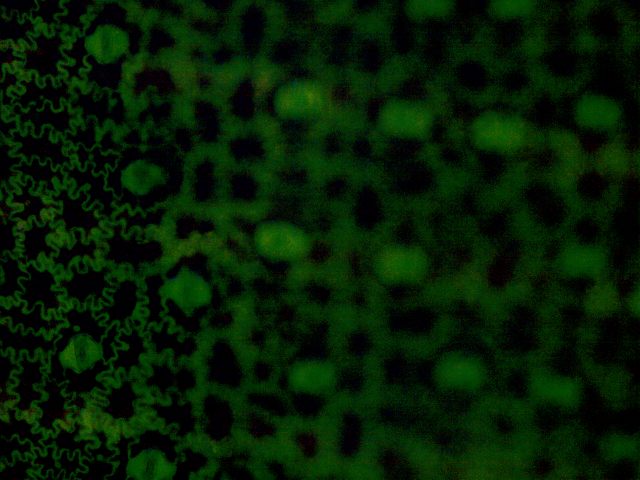
\includegraphics[scale=0.31]{images/cthenante_left.png}
        \caption{}
    \end{subfigure}%
    ~ 
    \begin{subfigure}[t]{0.45\textwidth}
        \centering
        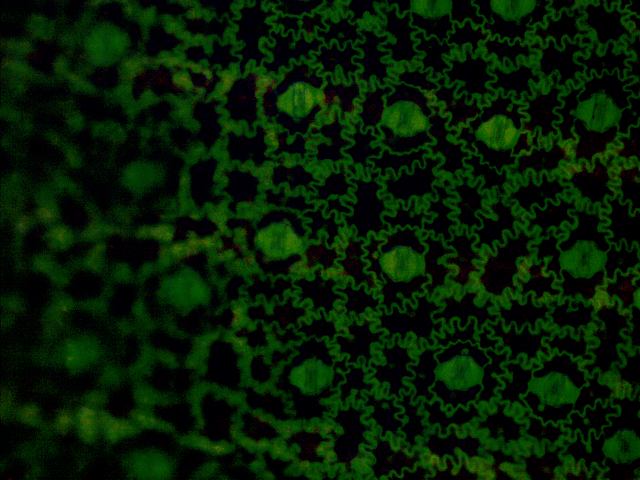
\includegraphics[scale=0.31]{images/cthenante_right.png}
        \caption{}
    \end{subfigure}
    \centering
    \fautor
\end{figure}

Sharpness is a concern when it comes to the analysis of microscopy images in order to obtain conclusions. According to \citeonline{costa2019multi}, blurred regions in sputum smear microscopy images caused by the depth of field limit in the microscope affect the accuracy of bacilli detection. Several proposed methods address the sharpness problem in microscopy images based on image restoration techniques. As stated by \citeonline{ponti2016image}, the most frequently used iterative method in microscopic image restoration is the Richardson-Lucy algorithm. Some examples presented by \citeonline{sun2005autofocusing} consist of four classes: \emph{derivative algorithms}, \emph{statistical algorithms}, \emph{histogram-based algorithms} and \emph{intuitive algorithms}. Among these applications, derivative methods deserve more credit. The Fourier Transform proved itself to be effective for low or moderate noise levels; in highly noisy environments, the resulting images were not satisfactory \cite{richardson1972bayesian}. As a consequence, probabilistic methods based on the Bayes Theorem were developed and provided images with better contrast, higher bandwidth and edge enhancement for confocal fluorescence microscopy samples \cite{ponti2016image}.

The resulting images from such restoration processes are sharper than the observed ones. However, the algorithms produce degradation as output. An alternative to restoration is to use images from the same object, with different foci, in order to obtain an enhanced depth of field image with low degradation levels. This process is known as image fusion, and even though a significant effort was done by researchers towards the development of techniques in this context, most of the image fusion methods are applicable but not directly related and built for bright-field microscopy images. The fusion process also require the selection of images that have ate least some sharp region, and according to \citeonline{koho2016image}, very few publications that address the problems of measuring the quality of images can be found on microscopy applications. There are many image analysis tools, but not many easily accessible and applicable image quality assessment methods.


\section{Aims and Hypothesis}

This work aims to develop a method to perform the fusion of bright-field microscopy images acquired in different focal planes. We propose three stages to achieve this, described as follows:

\begin{itemize}
    \item \emph{Dataset acquisition}: Acquisiton of a bright-field microscopy image dataset of leaf samples to evaluate the performance of the methods;

    \item \emph{No-reference image quality assessment}: Development of a method to quantitatively assess the quality of bright-field microscopy images based on the Fourier transform and descriptive statistics; 
    
    \item \emph{Multi-focus image fusion}: Fusion of the sharp regions of selected images among the dataset by means of a Laplacian of Gaussian-based method and compose the sharp image.
    
\end{itemize}

It is hypothesized that frequency domain information from images may be used to quantify the sharpness of bright-field microscopy images. Simultaneously, we also have the hypothesis that image fusion methods that employ edge detection by means of the Laplacian operator and its derivatives, e.g. the Laplacian of Gaussian, perform well on bright-field microscopy images. 

\section{Contributions}

This work yields the bright-field microscopy z-stack datasets as a first contribution. Those may be used to study, develop and test novel no-reference image quality metrics and multi-focus image fusion techniques by image processing and microscopy researchers, as well as industry professionals. The datasets comprise real world high-resolution microscopy images of biological material (particularly, plant leaves) with different illumination techniques and settings, which turns image quality assessment and image fusion into more challenging tasks.

In addition to the datasets, our proposed quality index and fusion algorithms explore well-known mathematical analysis, image processing, signal processing and statistical techniques. This not only it provides significant applications of those tools, but also stimulates studies among researchers in order to combine new state-of-the-art technologies to strong theoretical concepts in order to develop robust and scalable solutions.

\section*{Structure of the document}

This monograph is organized as follows:

\begin{itemize}
    \item \autoref{chapter:fundamentals-of-optics-and-light-microscopy} provides the bright-field microscopy basics and the z-stacking technique, i.e. the method to acquire images in different focal planes;
    
    \item \autoref{chapter:blur-characterization-and-image-formation} comprises relevant information about the bright-field microscopy image formation process and also describes the defocus blur property;
    
    \item \autoref{chapter:theoretical-background} provides the theoretical basis of this work, i.e. Fourier transform, image enhancement, registration, fusion and quality assessment, as well as the statistical methods employed in the analysis;
    
    \item \autoref{chapter:related-work} presents methods in which this work is based on, by means of a literature review on no-reference image quality assessment and multi-focus image fusion;
    
    \item \autoref{chapter:materials-and-methods} presents the acquisition and usage protocols of the proposed image datasets and the proposed method;
    
    \item \autoref{chapter:results} presents our results with the proposed datasets and exposes a discussion concerning the quantitative and qualitative analysis of them;
    
    \item \autoref{chapter:conclusions} summarizes what has been achieved, suggests some future work on the field and improvements to the methods;
    
    \item
    \autoref{chapter:fundamentals-of-optics} presents fundamentals of optics that may aid the comprehension of bright-field microscopy;
    
    \item
    \autoref{chapter:theoretical-background-details} provides details about some of the background concepts;
    
    \item \autoref{chapter:definitions-and-proofs} is the result of mathematical reasoning to prove some properties concerning the method which were hypothesized true.
    
\end{itemize}

\chapter{Bright-field Microscopy Fundamentals}
\label{chapter:fundamentals-of-optics-and-light-microscopy}
Microscopes are instruments designed to accomplish several important tasks to human knowledge, capable of magnifying images of small objects and structures which otherwise would not be seen by the human eye. It grants more information about the object of study to the research or the analysis. The first idea of the device was introduced by Romans, which discovered the magnifying property of glass in some sort of biconvex shape. Zacharias Janssen (1588-1632) was responsible for the invention of the first compound microscope with a concave eyepiece and  Francisco Fontana (1580-1656) introduced the convex eyepiece version of it \cite{zilio2009optica}. Furthermore, Robert Hooke (1635-1703) and Anton van Leeuwenhoek (1632-1723) were the most prominent science-related men responsible for microscope improvements \cite{wu2008microscope}.

Science is subject to continuous technological improvements that reflect on every field of study. Due to the development of theories and their empirical proofs of veracity, in addition to the advances in hardware and software power, techniques such as image processing are applied to other fields. This also happens in microscopy, aiming to improve image quality, data reliability, and range of use \cite{boyde1990modern}.

This chapter provides information about optics and microscopy concepts in this work. The first part is dedicated to the basic set of concepts and properties from optics that are necessary for light microscopy; the second one describes the structure of the optical microscope, along with its uses and implications on the acquired images. Plenty of image degradation is due to the system acquisition process; in fact, defocus is a natural occurrence in optics, mainly caused by adjustments of the optical system.

% \subsection{Properties of the Spherical Lenses}
% Within the scope of this work, the main reason for introducing the concepts of optics is the imaging devices - the microscope, in particular. The structure of the apparatus will be described in Section \ref{sec:light_microscopy}. Moreover, a substantially large amount of devices rely on optical lenses for imaging, with properties such as depth of field and depth of focus.

As stated by \citeonline{halliday2013fundamentals}, \emph{lenses} are objects consisting of a transparent material, with a certain refractive index, that are made of two spherical surfaces on which light propagates and suffers refraction. They are used in optical systems due to their capacity to create images as long as their refractive index is not equal to that of the medium. Still, in agreement with \citeonline{halliday2013fundamentals}, some concepts related to lenses are important in our context and will be shown below. The following list depicts the principal elements from geometric optics that relates to lenses and its consequent imaging properties:

\begin{itemize}
    \item \emph{Radius of Curvature}: the distance between the center of the sphere and a refracting surface, named $\mathit{r_{1}}$ and $\mathit{r_{2}}$ on Figure \ref{fig:spherical_lens};
    
    \item \emph{Center of Curvature}: since the lenses are made by a union of two sections of a sphere-shaped object (which have a center), there are two Centers of Curvature for each lens, denoted by $\mathit{C_{1}}$ and $\mathit{C_{2}}$ on Figure \ref{fig:spherical_lens};
    
    \item \emph{Central Axis}: a line that represents the infinite number of radii of the sphere, which contain the center and the focal point;
    
    \item \emph{Focal Point}: also called \emph{focus}, a point within the central axis, where the image of the object is formed due to the convergence of the light rays from the object, and shown on Figure \ref{fig:spherical_lens} as $\mathit{F_{1}}$ and $\mathit{F_{2}}$;
    
    \item \emph{Focal Length}: presented as $\mathit{f}$ on Figure \ref{fig:spherical_lens}, it stands for the distance between the center of the sphere and the focal point;
    
    \item \emph{Object}: either a point or a surface on space that emits (or reflects) light and can be interpreted as a source;
    
    \item \emph{Image}: in this context, it is a representation of an object, formed by the action of lenses.
    
    \item \emph{Magnification}: a number that describes how larger or smaller the image will be in comparison to the object; mathematically, the ratio of the image distance to the object distance, both relative to the lens.
    
\end{itemize}

A single lens or a set of lenses (most of the optical systems are more complicated than a single lens) have the \emph{depth of field} and the \emph{depth of focus} properties. Although the terms appear to be similar, the former relates to objects and the latter, to images \cite{davidson2002optical}. For every system, there is a focal plane in which the formed images will be sharp. Depth of Field is the tolerance for the object focal plane that may produce sharp images, while Depth of Focus dictates the same tolerance for the image focal plane. In other words, depth of field is the zone in the real world that would yield an acceptably sharp image and depth of focus is the same idea for the imaging sensors or for plotting the image.Figure \ref{fig:spherical_lens} denotes an illustration of an arbitrary spherical lens.

\begin{figure}[htb]
	\centering
	\caption{\label{fig:spherical_lens} Arbitrary scheme of the optical properties of a spherical lens.}
	\begin{center}
	    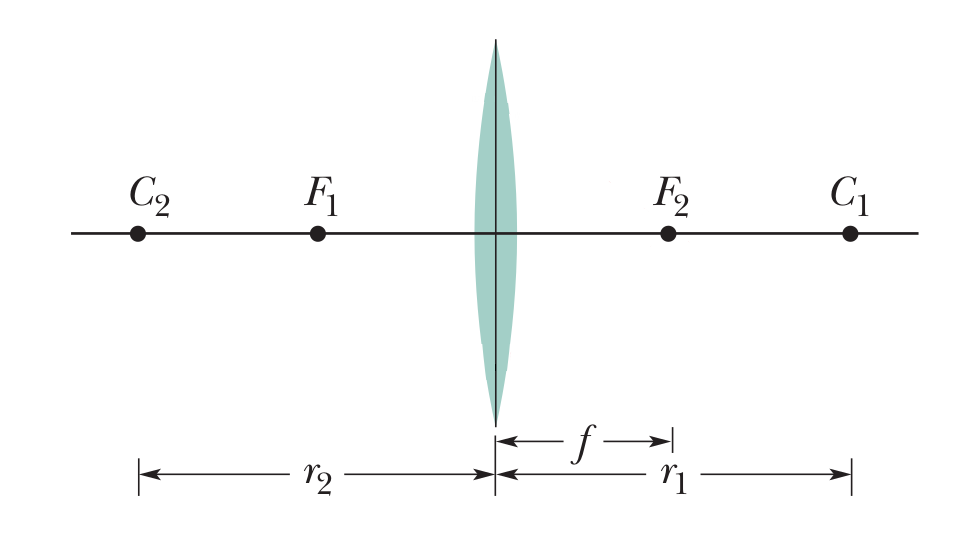
\includegraphics[scale=0.4]{images/fig4.png}
	\end{center}
	\centering
    \fadaptada{halliday2013fundamentals}
\end{figure}

Some properties of the spherical lenses directly influence the image formation process and, consequently, the resulting image quality. The \emph{numerical aperture}, as reported by \citeonline{murphy2012fundamentals}, is a measurement in terms of angles that shows how much lenses can capture light, and is given by

\begin{equation}
    \label{eqn:numerical_aperture}
    NA = n \sin{\theta},
\end{equation}

\noindent where $\theta$ is the half angle of the cone of specimen light accepted by the objective lens and $n$ is the refractive index between the lens and the specimen. There are optical flaws in lenses that hinder a proper image formation. Those are named \emph{aberrations} \cite{lawlor2019introduction}, and the most relevant types in the scope of this project are the \emph{spherical aberrations}. According to \citeonline{murphy2012fundamentals}, the spherical aberrations occur when there is a difference in the focal point of incident parallel rays at central and peripheral locations of a spherical lens' surface, which yields a blurred image of either a point source of light or an extended object. It is possible to correct a spherical aberration by changing the shape of the refracting surface, i.e. changing the radius of curvature for the lenses in order to adjust the focal point to one particular distance \cite{smith1988optics}. The illustration in Figure \ref{fig:spherical_aberrations} represents the spherical aberration for a point source of light, where it is possible to see the difference between incident rays in the borders and in the inner regions of the lens. The resulting image is, in this case, a set of concentric circles around a point.

\begin{figure}[htb]
	\centering
	\caption{\label{fig:spherical_aberrations} Arbitrary example of the spherical aberration.}
	\begin{center}
	    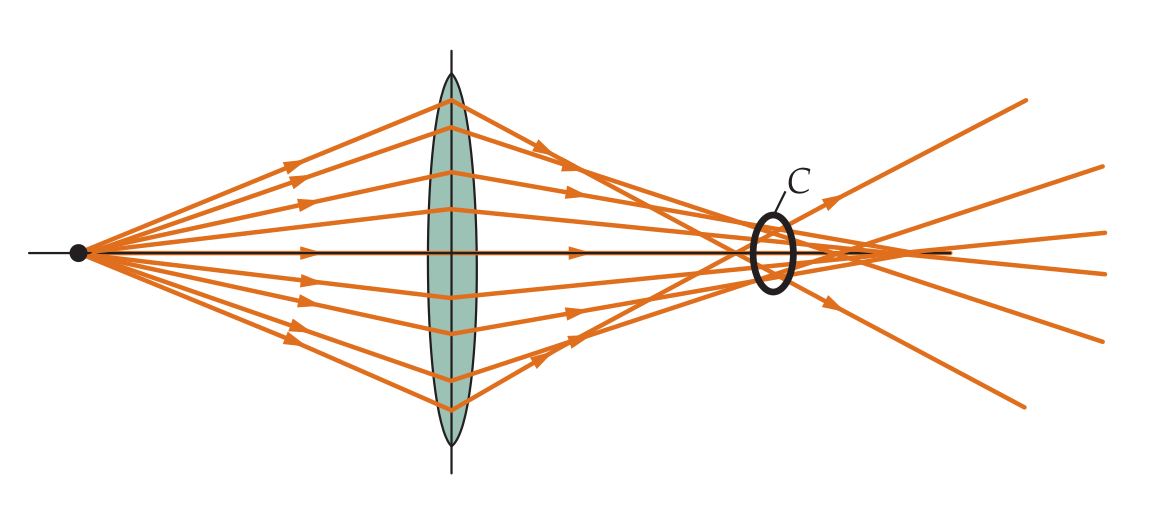
\includegraphics[scale=0.3]{images/spherical_aberration.png}
	\end{center}
	\centering
    \fdireta{tipler2008physics}
\end{figure}
    
\section{Bright-field microscopy}
\label{sec:light_microscopy}

Historically, the structure of the first microscopes developed by Hooke and Leeuwenhoek had no eyepiece; the compound microscope, developed by Janssen, consists of the magnification lenses and also an eyepiece, which adds more magnification power and delivers the image to the user \cite{lawlor2019introduction}. As stated by \citeonline{murphy2012fundamentals}, the word \emph{compound} refers to the fact that the objective lens and the eyepiece (or ocular) work together to produce the final magnification of the image as a product of their magnifications. A graphical representation of the general structure of a compound microscope is shown in \autoref{fig:compound_microscope}, and as reported by \citeonline{bell2009introduction}, it consists of objective lenses, eyepieces, condensers, the stage and the light source.

\begin{figure}[H]
	\centering
	\caption{\label{fig:compound_microscope} Structure of the basic compound microscope: lenses that capture light rays from the specimen or object (objectives) or where the observer may look through (eyepieces), a collector of light from the light source (condenser), the support for the object (stage) and the light source.}
	\begin{center}
	    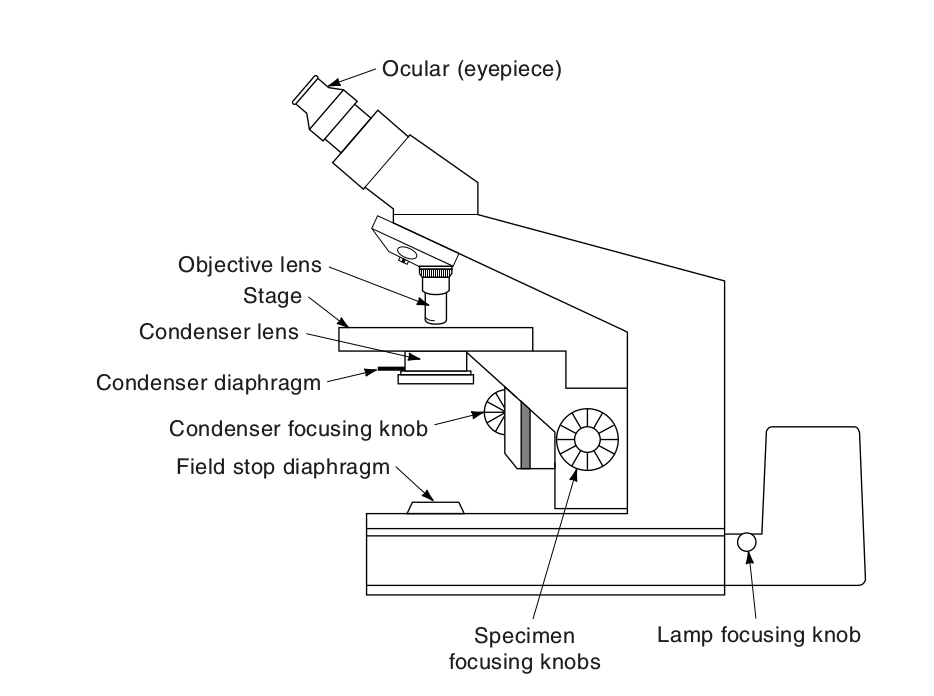
\includegraphics[scale=0.4]{images/fig5.png}
	\end{center}
	\centering
    \fdireta{bell2009introduction}
\end{figure}

Since light is some sort of radiation, there are several different ways to achieve imaging in microscopes; it can be made by light, polarized light, lasers, X-rays, among others. There are also advanced techniques such as confocal microscopy, which is capable of imaging a very small area of the object, with all the light rays focused on it \cite{rochow1994introduction}. The choice of the most suitable microscopy depends on the task.

According to \citeonline{dokland2006techniques}, the purpose of light microscopy is to provide magnified images of specimens by means of capturing emitted, reflected or transmitted light in the visible range of the spectrum, or even in the ultraviolet or near-infrared regions. As reported by \citeonline{lawlor2019introduction}, there are three general styles of light microscope. The \emph{upright microscope} is the easily affordable, easy to use traditional configuration with a light source on the base, a stage and the objective lenses. The \emph{inverted microscope} consists of the inverted configuration of an upright microscope, and offers some advantages when it comes to life sciences applications such as live cell imaging. Finally, the \emph{stereomicroscope} consists of a fusion of two compound microscopes in a convergent optical system and may have two different objectives and eyepieces or only one objective and two eyepieces \cite{schreier2004advances}. The former is named \emph{binobjective-binocular} (Greenough) and the latter \emph{monobjective-binocular}, or \sigla{CMO}{Common Main Objective Stereo Microscope}. One of the advantages of CMO microscopes is the higher depth of field, which allows the user to view and investigate biological specimens, relatively small materials and any kind of non-smooth surfaces. Furthermore, it is possible to view and acquire images in three dimensions \cite{rochow1994introduction}. The structure of both types of stereo compound microscopes is depicted in \autoref{fig:stereo_compound_microscope}.

\begin{figure}[htb]
	\centering
	\caption{\label{fig:stereo_compound_microscope} Graphic representation of the basic stereo compound light microscope structure, (a) for the Greenough type and (b) for the CMO.}
	\begin{center}
	    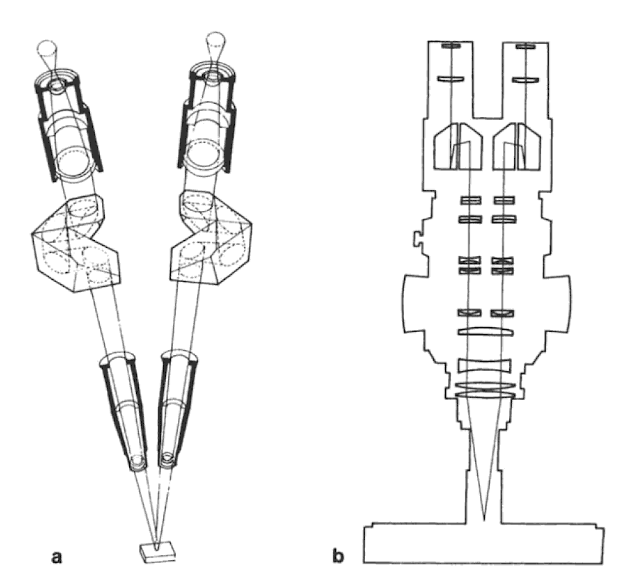
\includegraphics[scale=0.4]{images/stereomicroscope.png}
	\end{center}
	\centering
    \fdireta{rochow1994introduction}
\end{figure}

\subsection{Z-stacking Technique}
As for the use of light microscopes, there are several techniques and configurations which are achieved by varying the amount of lenses and light sources: bright-field, dark-field, phase-contrast, differential interference and fluorescence \cite{roane2009microscopic}. As stated by \citeonline{lawlor2019introduction}, images in bright-field microscopy are characterized by the contrast between the sample and the bright white background, generated by transmitted light. It is commonly used in pathology and histology fields for imaging fixed cells and tissues to reveal their structure, shape, and organization. The amount of light should be controlled, since the sample might suffer substantial changes, e.g. the chlorophyll molecules when illuminated by UV and visible light suffer irreversible breakdown (photodegradation) and generate other photoproducts \cite{petrovic2017clorophyll}. The \autoref{fig:bright-field_microscopy} provides an example of bright-field microscopy image.

\begin{figure}[htb]
	\centering
	\caption{\label{fig:bright-field_microscopy} Example of bright-field microscopy of a bone tissue.}
	\begin{center}
	    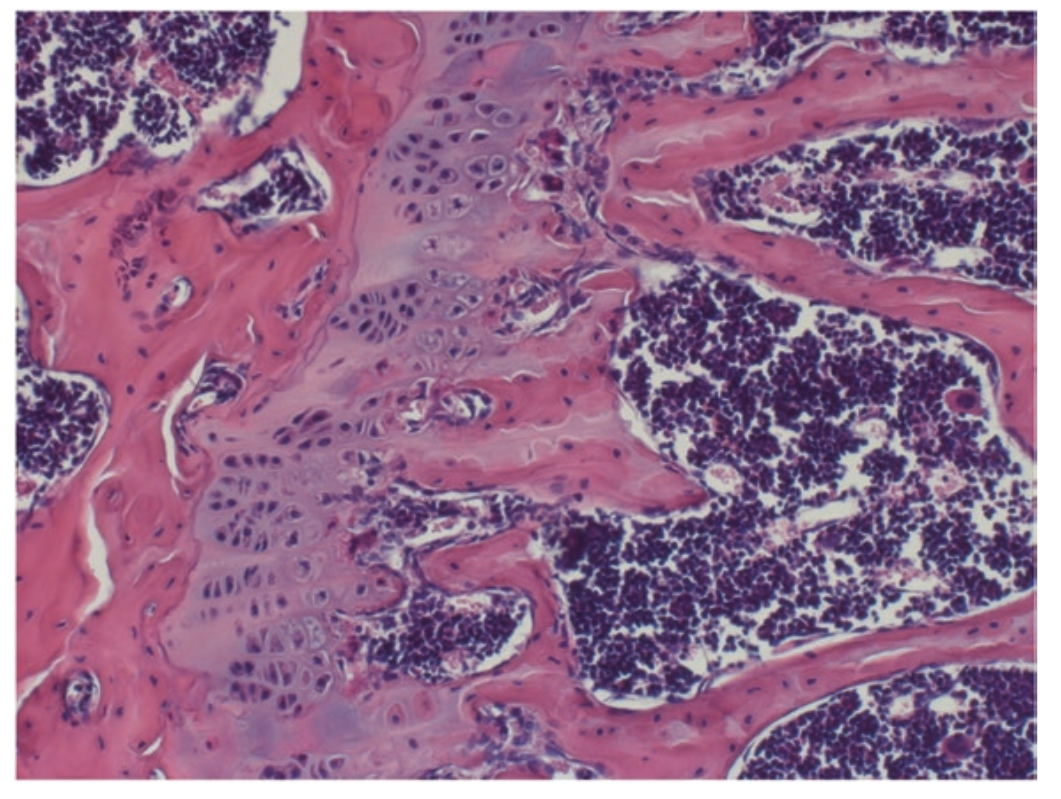
\includegraphics[scale=0.3]{images/bright-field_microscopy.png}
	\end{center}
	\centering
    \fdireta{lawlor2019introduction}
\end{figure}

The \textit{z-stacking} is a procedure to capture images in different positions concerning the $z$ axis, named slices, which may be applied to many different techniques to create a pseudo 3D image of the sample and consequently retrieve depth information about the specimen \cite{lawlor2019introduction}. The distance between each slice is dictated by the technique, either manually or automatically, and the focus needs to be adjusted at each slice. Next, the images must be aligned before any analysis is conducted. \autoref{fig:z-stack_example} represents a z-stacking example.

\begin{figure}[H]
	\centering
	\caption{\label{fig:z-stack_example} Z-stack images of yeast cells, acquired in positions under the focal plane (-15, -10 and -5 $\mu m$), exactly on it (0 $\mu m$) and above it (5, 10 and 15 $\mu m$).}
	\begin{center}
	    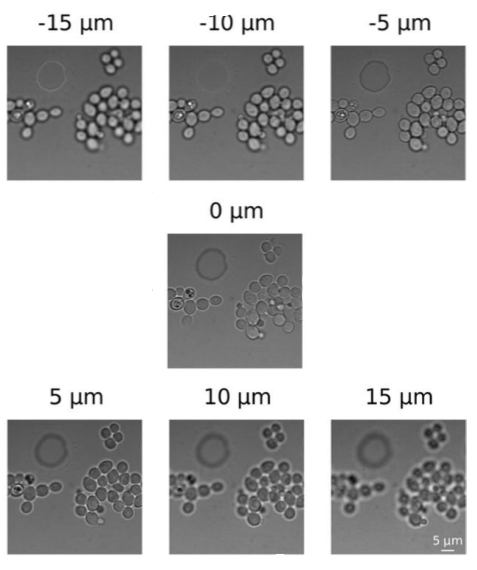
\includegraphics[scale=0.5]{images/z-stack.png}
	\end{center}
	\centering
    \fadaptada{wei2018neural}
\end{figure}

\chapter{Image Formation and Defocus Blur}
\label{chapter:blur-characterization-and-image-formation}
%%%%%%%% symbols to add
\simbolo{f(x,y)}{Original image as a function of spatial coordinates $x$ and $y$}

\simbolo{g(x,y)}{Observed image as a function of spatial coordinates $x$ and $y$}

\simbolo{J_{1}}{Bessel function of the first kind}

% \simbolo{\eta}{Additive noise function}

% \simbolo{\ast}{Convolution operation}

% \simbolo{\delta}{Dirac delta function}

% \simbolo{\mathbb{R}}{Set of real numbers}

% \simbolo{\mathbb{N}}{Set of natural numbers}

% \simbolo{\wedge}{Diagonal matrix of decrescent multiple singular values}

% \simbolo{\mathbb{G} = (\mathbb{V},\mathbb{E})}{Graph}

% \simbolo{\mathbb{V}}{Set of vertices of a graph}


The human eye constructs images from incident light rays on the \emph{retina}, a very complex set of photoreceptors that converts light into electrical signals which are later interpreted by the brain. The result of this process may be modelled as continuous function of two variables $f(x,y)$ which comprises the \emph{illumination} and the \emph{reflectance} information, i.e. the amount of incident light and the amount of reflected light in the scene, respectively \cite{gonzalez2018digital}.

Digital image processing deals, as the name proposes, with \emph{digital images}, i.e. discrete representations of $f(x,y)$ generated by sensors that are capable of transforming the illumination and reflectance information into electric signals. Still according to \citeonline{gonzalez2018digital}, in order to achieve this representation, the signals undergo sampling (signal conversion from continuous to discrete) and quantization (mapping of real-valued intensities to discrete pixel values) processes. For the sake of notation simplicity, $f(x,y)$ denotes the digital image and the term ``image'' also refer to it along this work.

It is clear that the image formation is influenced by several factors: sensor type, scene illumination conditions, and others. Indeed, each imaging system such as a camera or a microscope adds its own constraints to the process, e.g. conventional transmitted light microscopy images are only achieved with non-opaque samples \cite{rudi2020contrast}. Although there are many types of microscopy with different imaging procedures, this work limits its scope to bright-field microscopy. Therefore, this chapter summarizes the bright-field microscopy image formation processes and its implications on quality of the images. Furthermore, it describes blur properties concerning its origins either in image formation or other events. 

\section{Image Formation}
As mentioned in \autoref{chapter:fundamentals-of-optics-and-light-microscopy}, the bright-field microscopy images are formed by either transmitted or reflected light that passes through the sample and reach the objective lens. There difference between transmitted light and reflected light microscopes is the illumination system; there is no difference in how both direct light rays after those leave the specimen \cite{leng2009materials}.

According to \citeonline{davidson2002optical}, the light which reaches the specimen is either undeviated, i.e. does not suffer any disturbances in its direction, or diffracted; the diffracted rays leave the sample with a phase difference of 180 degrees in comparison to the undeviated light and cause destructive interference in the eyepiece, which projects a magnified version of this pattern onto a sensor and consequently produces the image.

Furthermore, the diffraction patterns that are captured by objectives have a particular shape. Still as stated by \citeonline{davidson2002optical}, the \emph{Airy disks}(also called \emph{Airy patterns}), named after Sir George Biddell Airy (1801 - 1892), are small circular diffraction disks projected by the objectives onto the image plane of the eyepiece diaphragm, which describe the focus profile the resulting image. The Airy disks as described by \citeonline{fowles1989introduction} follow the Fraunhoffer diffraction pattern, and may be mathematically modelled as an angular distribution of intensity of light diffracted by a circular aperture, given by

\begin{align}
\label{eqn:airy_function}
I(\theta) = I_{0} 
            \left[ 
            \frac{2 J_{1} (\rho)}{\rho}
            \right]^{2}
&&
\rho = \left( 
        \frac{2 \pi \sin{\theta}}{\lambda}
        \right) \frac{a}{2},
\end{align}

\noindent where $I_{0} = (C \pi R^{2})^{2}$ is the intensity for $\theta = 0$, $C$ is a constant, $R$ is the radius of the aperture, $\lambda$ is the wavelength of the light, $a$ is the diameter of the aperture and $J_{1}$ is the Bessel function of the first kind and first order \cite{mathews1970mathematical}, where the general case for the $rth$ order is given by

\begin{align}
\label{eqn:1st_bessel}
J_{r}(x) = \sum_{n = 0}^{\infty}
            \frac{(-1)^{r}}
                 {r! \Gamma(m + r + 1)}
            \left(
                \frac{x}{2}
            \right)^{m + 2r}
&&
\Gamma(z) = \int_{0}^{\infty} e^{-u} u^{z-1}du.
\end{align}

The Airy disks are intrinsically related to the numerical aperture and the definition of \emph{resolution}. The resolution is the minimum distance between two points at which they can be visibly distinguished as two points; optically, it is defined as the minimum distance between two Airy disks that can be distinguished, which is limited by diffraction \cite{leng2009materials}. The resolution of an optical microscope, given by the Rayleigh equation, is described by

\begin{equation}
\label{eqn:resolution}
d = 1.22 \frac{\lambda}{2 NA},
\end{equation}

\noindent where $d$ is the space between two adjacent particles that may be distinguished from each other, $\lambda$ is the wavelength of the illumination and $NA$ is the numerical aperture of the objective \cite{davidson2002optical}. It is evident that objectives with higher numerical apertures and shorter wavelengths of visible light will yield better resolution. \autoref{fig:airy_disks} shows arbitrary examples of Airy patterns, as well as their possible configurations and their consequences to the image. In \autoref{fig:airy_disks}.(a), the usual shape of Airy patterns is shown, together with its two-dimensional representation as a function of the intensity by an interval. Next, \autoref{fig:airy_disks}.(b) depicts an occurrence of Airy disk overlapping where both points would be properly resolved, i.e. below the Rayleigh limit, and \autoref{fig:airy_disks}.(c) represents the minimum distance in which both points would be distinguished. Finally, \autoref{fig:airy_disks}.(d) represents an unresolved pair of points.

\begin{figure}[htb]
	\centering
	\caption{\label{fig:airy_disks} Arbitrary example of an Airy disk (a), resolved Airy disks (b), Rayleigh limit of resolution (c) and unresolved Airy disks (d).} 
	\begin{center}
	    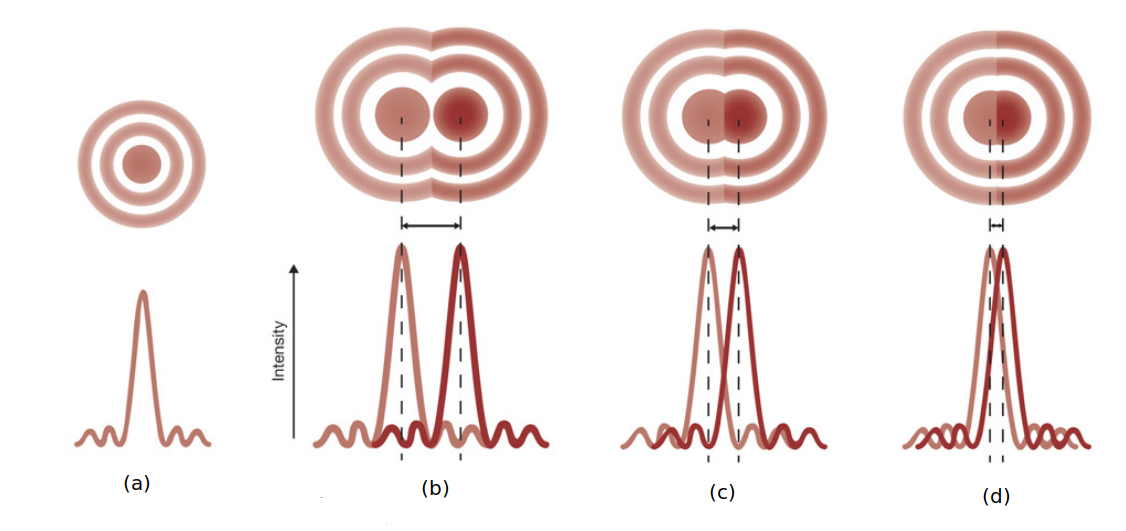
\includegraphics[scale=0.4]{images/airy_disks.png}
	\end{center}
	\centering
    \fadaptada{dunst2019imaging}
\end{figure}

As explained by \citeonline{goodman1996introduction}, an imaging system, particularly a set of microscope lenses, is said to be \emph{diffraction-limited} if the incident spherical light wave generated from a point-source object is transformed into another spherical wave which converges to an ideal image point, described by the original object point and affected by some sort of isotropic effect, such as magnification in a microscope.

The depth of field was described in \autoref{chapter:fundamentals-of-optics-and-light-microscopy} in terms of focal plane distances, but it may also be taken as the \emph{axial resolving power}, a measurement of resolution along the $z$ axis, determined by the numerical aperture and described by the Airy disk profile \cite{davidson2002optical}. Similarly to the Rayleigh's equation, the depth of field increases
with higher numerical apertures for the objective and shorter wavelengths of the incident light, and it represents a key property concerning the amount of blur in the resulting image.


\subsection{Point Spread Function and Image Formation Model}

\label{sec:point_spread_function_and_image_formation_model}

When light waves from a point source reach lenses, they suffer diffraction and refraction, which construct a new propagating set of rays that converge to a point in the center of the image plane in the shape of Airy disks; such shape is called the \sigla{PSF}{Point Spread Function}
of the imaging system (also called \emph{impulse response}), and it is intrinsically related to the imaging process \cite{wu2008microscope}. Particularly, the bright-field microscopy employs polychromatic nonpolarized incoherent light. From this concept, it is possible to relate the Airy disks to the PSF, since those are intensity distributions for each point source of light emanating from the specimen. \autoref{fig:point_spread_function}.(a) presents a theoretical scheme of imaging for a point source of light, and \autoref{fig:point_spread_function}.(b) depicts the shape of a incoherent PSF:

\begin{figure}[htb]
	\centering
	\caption{\label{fig:point_spread_function} Point Spread Function generated by a focused diffraction-limited system with incoherent light.} 
	\begin{center}
	    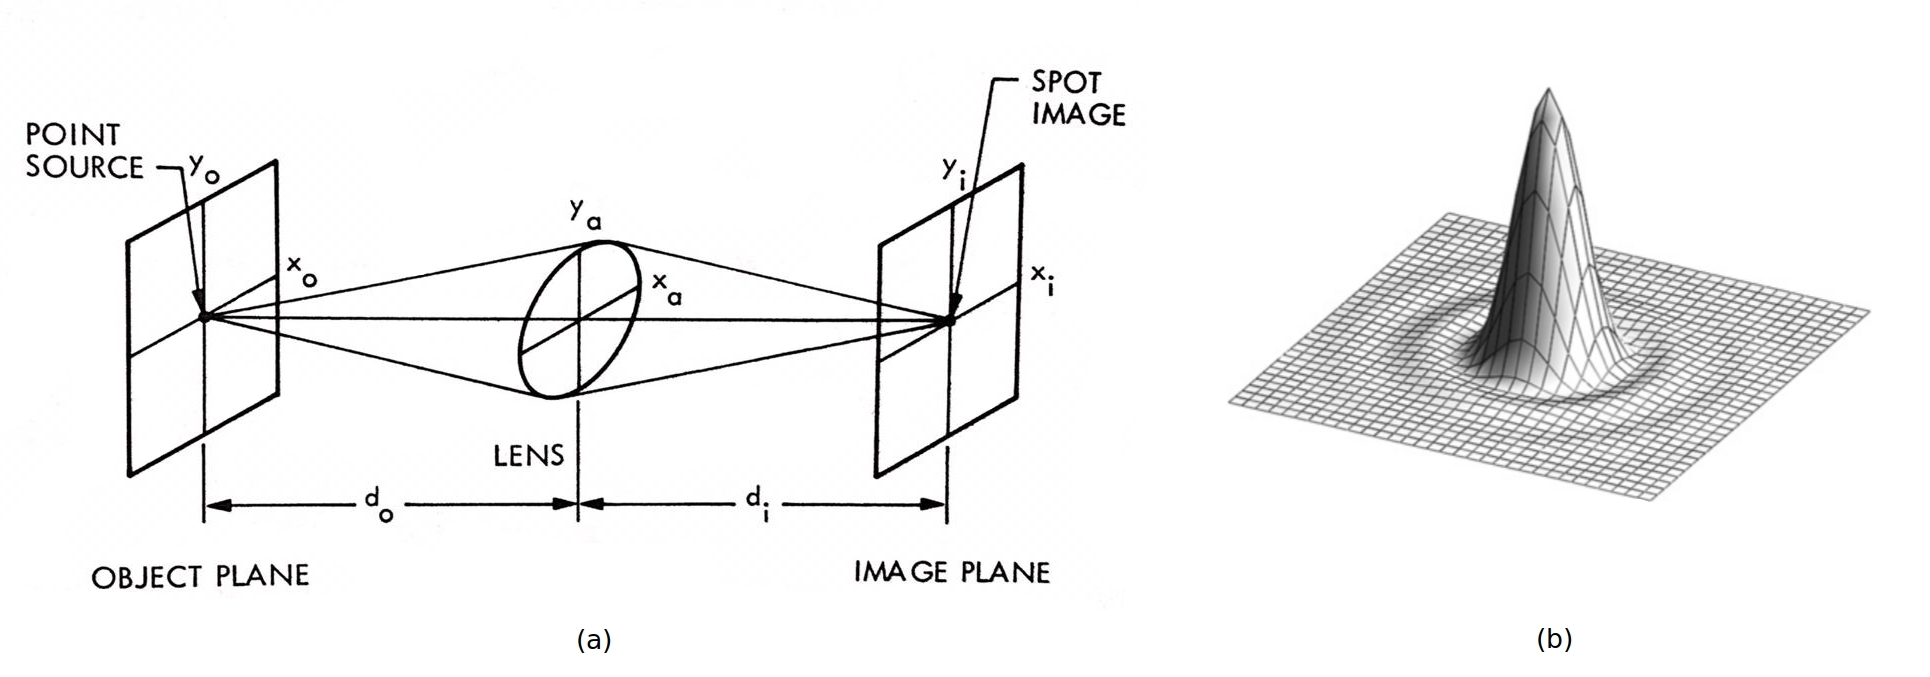
\includegraphics[scale=0.235]{images/point_spread_function.jpeg}
	\end{center}
	\centering
    \fadaptada{castleman1996digital,wu2008microscope}
\end{figure}

In \autoref{fig:point_spread_function}.(a), the imaging system in in focus, which is given by

\begin{equation}
\label{eqn:lens_focus}
\frac{1}{d_{o}} + \frac{1}{d_{i}} = \frac{1}{f},
\end{equation}

\noindent where $f$ is the focal length of the lens, $d_{o}$ and $d_{i}$ are respectively the distances from the point source plane to the lens and the distance from the image plane to the lens; the intensity of light in the point source is directly proportional to the intensity in the image, what characterizes a \emph{two-dimensional linear system} \cite{castleman1996digital}. Still according to \citeonline{castleman1996digital}, any motion of the point source on its plane moves the image is dictated by the law

\begin{align}
\label{eqn:isoplanatic_motion}
x_{i} = -\frac{d_{i}}{d_{o}}x_{o}
&&
y_{i} = -\frac{d_{i}}{d_{o}}y_{o},
\end{align}

\noindent where $(x_{o},y_{o})$ are the coordinates for the object location on its plane and $(x_{i},y_{i})$ are coordinates that locate the image on its plane. This implies that the shape of the image will not change according to the object's location, and this property yield \emph{shift invariance} to the system, which may be called \emph{isoplanatic}. These properties are observed in an ideal imaging system - simple lenses are not isoplanatic and linear, and  consequently simple microscopes also. However, there are approximations and mathematical tools that allow advanced microscopes to be assumed isoplanatic and linear.

The PSF as related to the intensity distributions described by the Airy disks are limited to the area of the aperture. This means that the amount of light that reaches the image plane is truncated by the circular aperture, what is also true for the PSF. The truncation is mathematically represented by the \emph{pupil function}, which is zero outside the boundaries of the aperture and unity otherwise, and might include also information about wave aberrations of the lens \cite{goodman1996introduction}. As denoted by \citeonline{wu2008microscope} with some notation adjustments, the PSF of an incoherent illuminated circular aperture imaging system is the Fourier Transform (explained further in \autoref{chapter:theoretical-background}) of the generalized pupil function, given by

\begin{equation}
\label{eqn:incoherent_psf}
h_{\lambda}(x,y,z) = \int_{-\infty}^{\infty}
                     \int_{-\infty}^{\infty}
         P(u,v)
         e^{j 2 \pi z
            \left(
                \frac{u^{2} + v^{2}}{2 \lambda L^{2}}        
            \right)
        }
        e^{j 2 \pi
            \left(
                \frac{xu + yv}{\lambda L}        
            \right)
        }
        du dv,
\end{equation}

\noindent where $h_{\lambda}(x,y,z)$ is point spread function for a light with wavelength $\lambda$, $P(x,y)$ is the pupil function, $z$ is the axial location the focal plane and $L = r / NA$ is the focal length, i.e. ratio between the radius of the circular aperture of the objective and the numerical aperture. The normalized Fourier Transform of the PSF is called \sigla{OTF}{Optical Transfer Function} \cite{castleman1996digital}.

From this framework, the image is formed as a set of impulse responses from each point in the object plane that where magnified by the imaging system. Linear systems possess a general expression, a convolution (which will be explained in \autoref{chapter:theoretical-background}) of the input with the system's impulse response, that describes the output \cite{brigham1988fast}. In this sense, the resulting image is a convolution of the PSF with the original image, defined as

\begin{equation}
\label{eqn:image_formation_convolution}
g(x,y) = \int_{-\infty}^{\infty}
         \int_{-\infty}^{\infty}
         h(x-u, y-v)f(x,y)du dv,
\end{equation}

\noindent where $f(x,y)$ is the original image, $g(x,y)$ is the observed image, $h(x,y)$ is the PSF of the imaging system and $u,v$ are shift parameters.

\subsection{Discrete Image Formation Model}

Digital images follow a discrete model for image formation due to the acquisition process: the spherical waves that leave the objectives reach the surface of \sigla{CCD}{Charge-coupled Devices}, sensors which proportionally converts light intensities to electrical signals that digitized as pixels \cite{gonzalez2018digital}. The digital images are matrices of pixels that represent light intensities with different channel configurations, where the most common one is the \sigla{RGB}{Red, Green and Blue} image. Therefore, similarly to the image formation model shown in \autoref{sec:point_spread_function_and_image_formation_model}, the two-dimensional digital image formation is described with a discrete process, arbitrarily as

\begin{equation}
\label{eqn:discrete_image_formation}
g[x,y] = h[x,y] \ast f[x,y],
\end{equation}

\noindent where $\ast$ denotes the discrete convolution, $g$, $h$ and $f$ are respectively the observed image, the discrete PSF of the imaging system and the original image, and $x,y \in \mathbb{Z}$. The discrete PSF of an imaging system with incoherent illumination and a circular aperture is given by

\begin{align}
\label{eqn:discrete_psf}
h(r) = \left[
        2
        \frac{J_{1}[\pi (r / r_{0})]}{\pi (r / r_{0})}
       \right]^{2},
&&
r = \sqrt{x^{2} + y^{2}},
&&
r_{0} = \frac{\lambda d_{i}}{a},
\end{align}

\noindent where $h(r)$ is the radially symmetrical PSF, $r$ is the radial distance, $r_{0}$ is a scaling factor, $J_{1}$ is the Bessel function of first order and first kind, $\lambda$ is the wavelength of the illumination, $a$ is the diameter of the aperture and $d_{i}$ is the distance from the lens plane to the image plane. A scheme of the geometric setup of discrete image formation through the PSF is shown in \autoref{eqn:discrete_image_formation}: 

\begin{figure}[htb]
	\centering
	\caption{\label{fig:discrete_psf_scheme} Geometric scheme of a lens' circular aperture and arbitrary point spread function profile.} 
	\begin{center}
	    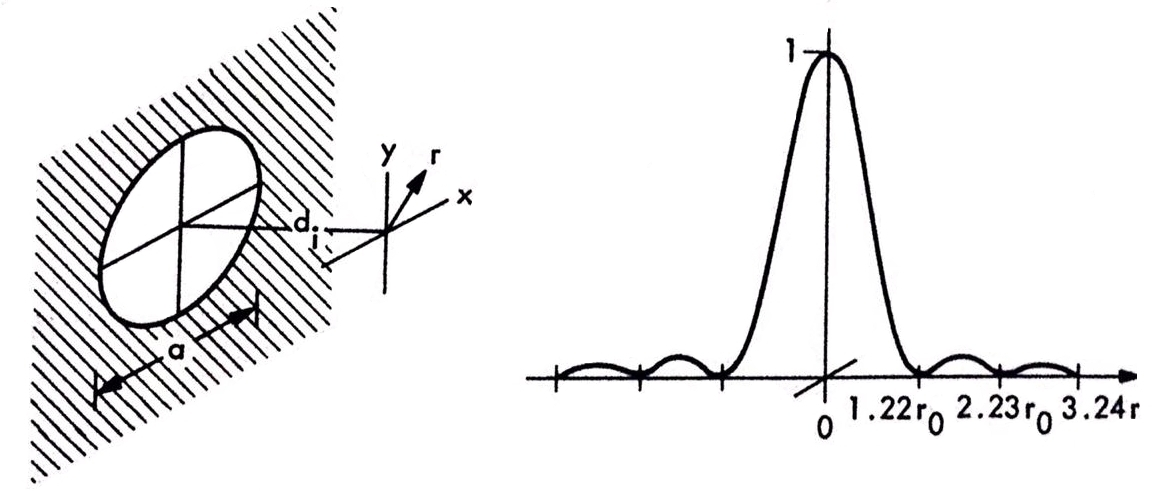
\includegraphics[scale=0.35]{images/discrete_psf_scheme.jpeg}
	\end{center}
	\centering
    \fadaptada{castleman1996digital}
\end{figure}

The discrete OTF is then the \sigla{DFT}{Discrete Fourier Transform} (explained in \autoref{chapter:theoretical-background}) of the PSF in \autoref{eqn:discrete_psf}. The OTF characterizes the intensities of light that emanate from the specimen in terms of frequencies. 

There is another property of image formation and acquisition that influences the image quality: the noise. Pursuant to \citeonline{wu2008microscope}, imaging is corrupted by intrinsic or extrinsic noise; the former is modelled by a Poisson distribution that influences each photon that reaches the sensor, and the latter is modelled by a Gaussian distribution that sums to the matrix of pixels. Details about noise are out of the scope of this work, since the degradation to be deeply explored is the defocus blur.

\section{Blur Characterization}
The \emph{blur} effect is one type of degradation that consists of global or local information loss in the image. There are three basic types of blur, generated by different processes: \emph{defocus blur}, \emph{motion blur} and \emph{Gaussian blur}. As explained in \autoref{sec:point_spread_function_and_image_formation_model}, the image formation process is subject to some constraints that limit its quality, such as the presence of noise or the convolution of the formed image with a point spread function. Such convolution results in defocus blur. 

The defocus blur is caused by the incidence of light within an aperture with significant dimensions, where the source of light is not properly placed in accordance to the focal plane; it is related to the variables of the optical system such as depth of focus, aperture, depth of field, aberrations and so on \cite{joshi2014defocus}. According to \citeonline{smith2007modern}, every optical system exhibits blur properties, in higher or lower proportions, due to the depth of focus and its adjustment. Therefore, blurring is unavoidable to a certain extent, hence every imaging device possesses a PSF due to its optics. The PSF is also named \emph{blur kernel}.

The motion blur occurs due to the relative motion between the camera and the scene, e.g. living cells in microscopy, during the acquisition; even though it is considered to be a degradation process, it may be used for aesthetic purposes, such as emphasizing the dynamic nature of a scene, obtaining motion information about the object or creating realistic images which are pleasing to the eye \cite{nayar2004motion}. Motion blur is usually an undesirable effect when it comes to fields such as microscopy, remote sensing or medical imaging, since it compromises analyses, pattern recognition tasks, predictions and several other applications.

The Gaussian blur is a general model of degradation and employs a particular kernel in order to smooth images. A convolution with such kernel promotes a Gaussian average among each region, and is usually employed in photography for styling effects or in edge detection (this application will be explained further in this work). Its kernel \cite{nixon2019feature} is given by

\begin{equation}
\label{eqn:gaussian_blur}
k(x,y) = e^{-
            \left( 
                \frac{x^{2} + y^{2}}{2 \sigma^{2}}
            \right)
            },
\end{equation}

\noindent where $\sigma^{2}$ is the variance of the Gaussian function. \autoref{fig:defocus_motion_blur} shows an example of large scale defocus and motion blur.

\begin{figure}[H]
	\centering
	\caption{\label{fig:defocus_motion_blur}Defocus blur (left) and motion blur (right) in large scales.}
	\begin{center}
	    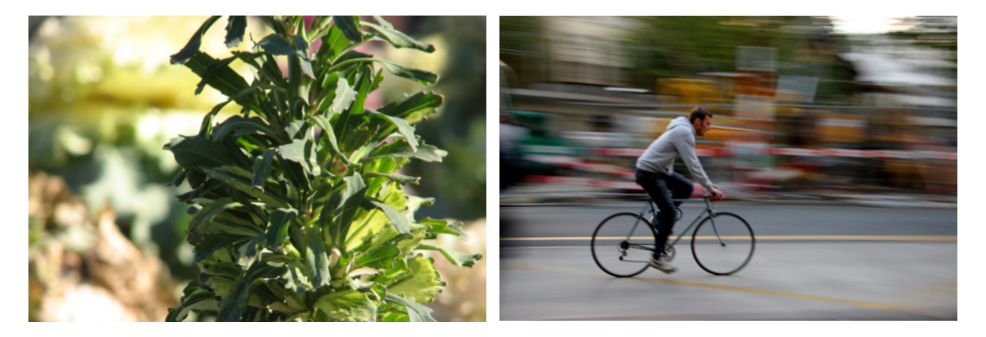
\includegraphics[scale=0.4]{images/fig7.png}
	\end{center}
	\centering
    \fadaptada{su2011blurred}
\end{figure}

Finally, another useful way to mathematically describe the point spread function is through the Dirac Delta. It consists of a generalized function that represents an impulse, i.e. an infinitely high value within an infinitely small period of time \cite{bracewell2000fourier}. \autoref{fig:psf} shows an arbitrary example of a punctual source of light and its image, which suffers the spreading effect.

\begin{figure}[H]
	\centering
	\caption{\label{fig:psf} Magnified image of a light impulse (left) and its impulse response function, the PSF (right).}
	\begin{center}
	    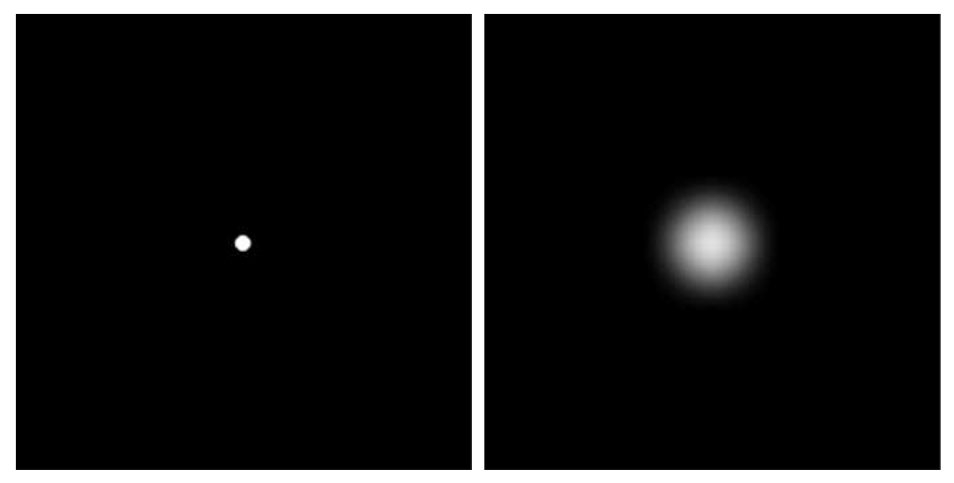
\includegraphics[scale=0.4]{images/fig8.png}
	\end{center}
	\centering
    \fadaptada{gonzalez2008digital}
\end{figure}

Namely, it is a function $\delta(x)$ that is zero-valued for any $x \neq 0$ and is infinity-valued for $x = 0$. This property can be combined with any smooth function $f\colon \mathbb{R}^{n} \to \mathbb{R}^{n}$.
The continuous Dirac Delta may be written, as stated by \citeonline{weisstein2020delta}, as

\begin{align}
\label{eqn:dirac_delta_function}
\delta^{2}(x,y)= 
\begin{cases}
    \infty, & \text{if } x^{2} + y^{2} =0\\
    0, & \text{if } x^{2} + y^{2} \neq 0
\end{cases},
&&
\int_{-\infty}^{\infty}
\int_{-\infty}^{\infty}
\delta^{2}(x,y)dxdy = 1.
\end{align}

\noindent The discrete version of the Dirac Delta function consists of an infinite sum instead of the integral. This concept of impulse is the point source of light, concerning images. It provides the blurring effect on images, as it promotes the diffusion of the acquired information.


\chapter{Theoretical Background}
\label{chapter:theoretical-background}
\simbolo{\ast}{Convolution}

This chapter summarizes the relevant theoretical concepts, methods, and tools for the development of our approach to select partially sharp images among a z-stack dataset and merge the best information from each selected image into a high-quality image. The mathematical and image processing concepts needed to develop our method are convolutions, transforms, enhancement, registration, fusion and quality assessment; statistical methods are used as a bridge between yielding a quantitative index of image quality and merging pixels, as well as evaluating the performance.

\section{Convolution and Image Transforms}
As seen in Chapters \ref{chapter:fundamentals-of-optics-and-light-microscopy} and \ref{chapter:blur-characterization-and-image-formation}, the processes of image formation and acquisition concerning linear systems are subject to some operations, i.e. the convolution, the \sigla{FT}{Fourier Transform} and its continuous and discrete versions, that modify the original representation of the scene. The linear system theory provides mathematical tools to explore those operations and others, such as sampling, filtering, and enhancement; it describes the behavior of electrical circuits and optical systems \cite{castleman1996digital}.

According to \citeonline{bracewell2000fourier}, the convolution of two arbitrary functions $s$ and $t$ results in another function $r$ is, with notation adjustments, defined by the integral

\begin{equation}
\label{eqn:one_dimensional_convolution}
r(x) = \int_{-\infty}^{\infty}s(u) t(x - u) du,
\end{equation}

\noindent where $x$ is the one-dimensional coordinate and $u$ is a shifting parameter. In other words, this procedure is compared to moving a 180 degrees-rotated filter mask over the function values and computing the sum of products at each location \cite{gonzalez2018digital}. Hence, the shifting parameter represents the slide of the filter mask above the values. As seen in Chapter~\ref{chapter:blur-characterization-and-image-formation}, convolution is responsible for the image formation and acquisition processes, but it also covers several other applications, e.g. smoothing, sharpening and reducing noise in images. Similarly to the one-dimensional case and pursuant to \citeonline{castleman1996digital}, the two-dimensional convolution is denoted by

\begin{equation}
\label{eqn:two_dimensional_convolution}
r(x,y) = \int_{-\infty}^{\infty}
         \int_{-\infty}^{\infty}
         s(u,v) t(x - u, y - v) du dv,
\end{equation}

\noindent where $u$ and $v$ are shifting parameters, $\ast$ denotes the convolution. The \emph{spatial domain} is the subset of the real plane where functions like $r$, $s$ and $t$ are spanned, and $(x,y)$ as points within such subset are named spatial variables; consequently, any mathematical operation that employs pixels from this subset are named spatial domain techniques. Concerning the digital image processing applications, which deals with images as matrices of pixels, the discrete two-dimensional convolution for an image $f(x,y)$ and a function $h(x,y)$ is given by 

\begin{equation}
\label{eqn:2d_discrete_convolution}
g(x,y) = h(x,y) \ast f(x,y) = 
        \sum_{m=-a}^{a}
        \sum_{n=-b}^{b}
        f(m,n) h(x-m,y-n),
\end{equation}

\noindent where $a = (m-1)/2$ and $b = (n-1)/2$, given that the function $h(x,y)$ is considered to be a two-dimensional filter of size $m \times n$ \cite{gonzalez2018digital}.

Convolution, together with several other operations employed in this work, operate directly on the spatial domain by modifying pixel values based on mathematical constraints. Some of those operations may have issues that hinder the operation, e.g. the computation time of a convolution process should be finite, otherwise, its use is impractical; this is one of the reasons why \emph{image transforms} are widely used. They encompass any group of mathematical operations that transfers the input signal or image from its domain to the transform domain \cite{gonzalez2008digital}. Let $s$ be an arbitrary two-variable function, $t_{f}$ and $t_{i}$ be the forward and inverse transformation kernels, respectively. The general discrete form of the forward and inverse two-dimensional transforms is denoted by 

\begin{align}
\label{eqn:generic_transform}
R(u,v) = 
\sum_{x=0}^{M-1}
\sum_{y=0}^{N-1}s(x,y)t_{f}(x,y,u,v)
&&
s(x,y) = 
\sum_{x=0}^{M-1}
\sum_{y=0}^{N-1}R(u,v)t_{i}(x,y,u,v),
\end{align}

\noindent where $M$ and $N$ are the dimensions of the image, $x$ and $y$ are coordinates of the image, $u = \{0,1,2,...,M-1\}$ and $v = \{0,1,2,...,N-1\}$ are called transform variables. The $t_{f}$ function is responsible for the forward domain change and the $t_{i}$ transfers the image back to the spatial domain. The domain switch allows different approaches to operations to be executed and present features of the image that could not be represented in the spatial domain. The convolution operation, for instance, turns itself into a simple matrix multiplication task on the Fourier Transform domain (which will be detailed in the following sections) and that solves the performance constraint.

\section{Continuous and Discrete Fourier Transform}
Regarding image transforms, one of the most important examples is the Fourier Transform. It was conceived by Jean Baptiste Joseph Fourier (1768 - 1830) and states that any periodic function can be expressed as the sum of sines and cosines of different frequencies, each multiplied by a different coefficient \cite{gonzalez2018digital}. According to \citeonline{brigham1988fast}, the relationship between the different frequency sinusoids and arbitrary function $s$ to be analyzed is described as

\begin{equation}
\label{eqn:fourier_transform}
S(f) = \int_{-\infty}^{\infty}s(x)e^{-j 2 \pi f x} dx,
\end{equation}

\noindent where $S(f)$ is the Fourier Transform of the $s(t)$ and $j = \sqrt{-1}$ represents the imaginary unit. Note that the function transformed from the one-dimensional spatial domain to the frequency domain, represented by $f$. Similarly, the inverse transform is denoted by

\begin{equation}
\label{eqn:inverse_fourier_transform}
s(x) = \int_{-\infty}^{\infty}S(f)e^{j 2 \pi f x} df.
\end{equation}

As stated by \citeonline{bracewell2000fourier}, an arbitrary periodic function $s$ with period $T$ is commonly to express it as a Fourier series, given by the expression

\begin{equation}
\label{eqn:fourier_series}
a_{0} + \sum_{1}^{\infty} (a_{n} \cos{2 \pi n f t} + b_{n} \sin{2 \pi n f t}),
\end{equation}

\noindent where

\begin{align*}
a_{0} &= \frac{1}{T} \int_{-\frac{1}{2} T}^{\frac{1}{2} T} s(t) dt\\
a_{n} &= \frac{2}{T} \int_{-\frac{1}{2} T}^{\frac{1}{2} T} s(t) \cos{(2 \pi n f t)} dt\\
b_{n} &= \frac{2}{T} \int_{-\frac{1}{2} T}^{\frac{1}{2} T} s(t) \sin{(2 \pi n f t)} dt.\\
\end{align*}

If the function is not periodic, then the Fourier Transform is applied as a continuous function of frequency, i.e. $s(t)$ is represented by the sum of sinusoids of all frequencies \cite{brigham1988fast}. Particularly, this stands for images, which are non-periodic functions. The common approach is to appraise the image as a section of a periodic function so the use of Fourier Transform makes sense.

The Equations \ref{eqn:fourier_transform} and \ref{eqn:inverse_fourier_transform} together are named a \emph{Fourier Transform pair}. Images are represented by two-variable functions, which motivates the use of a two-dimensional Fourier Transform; moreover, as digital images are matrix representations of images, the two-dimensional Discrete Fourier Transform is the most relevant brand of the FT for image processing applications. Consequently, the two-dimensional Fourier Transform pair of a function $s(x,y)$ is given by

\begin{align}
\label{eqn:two_dimensional_continuous_fourier_transform}
S(u,v) &= \int_{-\infty}^{\infty}
         \int_{-\infty}^{\infty}
         s(x,y) e^{-j 2 \pi 
                    \left(
                        ux + vy
                    \right)
                  }
        dx dy\\
s(x,y) &= \int_{-\infty}^{\infty}
         \int_{-\infty}^{\infty}
         S(u,v) e^{j 2 \pi 
                    \left(
                        ux + vy
                    \right)
                  }
        du dv.
\end{align}

According to \citeonline{bracewell2000fourier}, this pair of equations represents the analysis of $s(x,y)$ into components of the form $\exp{\left[j 2 \pi (ux + vy) \right]}$, where the variables $u$ and $v$ represent spatial frequencies. The equation that relates such components to sinusoids is the \emph{Euler's Formula} or \emph{Euler's Identity}, written as

\begin{equation}
\label{eqn:euler_formula}
    e^{j\theta} = \cos{\theta} + j\sin{\theta}
\end{equation}

\noindent where $\theta = 2 \pi f$ is a number that represents an angle in radians and $e^{j\theta}$ is the polar form representation of the sinusoids \cite{gonzalez2018digital}. Finally, the common two-dimensional DFT form applied among image processing is, as reported by \citeonline{gonzalez2018digital}, denoted by

\begin{align}
\label{eqn:two_dimensional_discrete_fourier_transform}
S(u,v) &= \sum_{x = 1}^{M}
          \sum_{y = 1}^{N}
          s(x,y) e^{-j 2 \pi 
                    \left(
                        ux/M + vy/
                    \right)
                  }
        dx dy\\
s(x,y) &= \frac{1}{MN}
          \sum_{1}^{M}
          \sum_{1}^{N}
          S(u,v) e^{j 2 \pi 
                    \left(
                        ux/M + vy/N
                    \right)
                  }
        du dv,
\end{align}

\noindent where $s(x,y)$ is a discrete function that represents an image of size $M \times N$, $x$ and $y$, discrete variables that represent spatial coordinates, $u$ and $v$ are discrete spatial frequencies. 

One prominent example of Fourier Transform use is the Convolution Theorem. It states that convolution may be computed by a multiplication in the Fourier domain \cite{brigham1988fast}. This allows much faster computations of convolution in comparison to the spatial domain approach and is frequently used in many applications, such as image filtering and convolutional neural networks. In terms of computational complexity, the common two-dimensional Discrete Fourier Transform implementations yield results in $\mathcal{O}(n^{2})$ time for square or zero-padded images and $\mathcal{O}(mn)$ for images of size $m \times n$; for this reason, the \sigla{FFT}{Fast Fourier Transform} is a divide-and-conquer implementation created by Cooley and Tookey in 1965 and reduces the computational complexity to $\mathcal{O}(n \log n)$ \cite{bracewell2000fourier}. The Fourier Transform is widely employed in this work and the chosen approach to compute it is the FFT algorithm.

\section{Image Enhancement}
With a clear panorama of convolution and Fourier transform concepts, it is possible to enlighten the \emph{image enhancement} concept and its relevant applications to this work. Image enhancement is the process of manipulating an image in order to provide a resulting representation that is more suitable for a particular problem, e.g. an enhancement method for medical images may not be efficient for satellite images \cite{gonzalez2018digital}. Within microscopy, image enhancement is desirable due to the limited capacity of optical imaging devices and also the features of each microscopy technique, e.g. acquisition with different illumination settings, focal planes, time intervals or spectral channels; hence, enhancement algorithms for microscopy should cover all types of information \cite{wu2008microscope}. According to \citeonline{wu2008microscope}, image enhancement techniques are divided into \emph{spatial domain}, \emph{Fourier transform} and \emph{wavelet transform} methods and will be described as follows. 

The spatial domain methods are basically transforms that globally maps the gray levels of an image (or the gray levels the channels from a multichannel image, such as RGB) to their enhanced stated. Some examples are contrast stretching, which adjusts all gray levels of an image to fit among the desired range, thresholding, which applies a decision function that creates a binary image based on a preset gray level, histogram equalization, and spatial filtering. Particularly, histogram equalization and spatial filtering play an important role in this work and therefore will be explored further.

Fourier transform domain methods operate with images as a distribution of frequencies since some features are better described by it. Noise, for example, may be suppressed in a sharpening process or reduced by amplifying mid-frequency components and attenuating high-frequency ones. The Wiener Filtering process is an extensively used example of a frequency domain enhancement method that recovers a noisy signal or image based on estimations of spectral properties from the original image. Other examples of Fourier domain enhancement are band-pass filters and least-squares deconvolution applications.

Finally, the wavelet transform based methods enhance images based on Wavelet Transforms, i.e. mathematical frameworks that decompose signals and images into frequency components in different scales. Some approaches such as thresholding may be applied to wavelet coefficients, and since the output of wavelet transforms depend on the chosen wavelet function, many possible variants depend on the image features. 

\subsection{Histogram Equalization}

The image histogram is one of the simplest and most useful tools in image processing and consists of a function that summarizes the gray level content of an image in terms of a frequency distribution \cite{castleman1996digital}. The histogram equalization consists of applying a non-linear monotonic mapping to provide an approximation of a uniform distribution to the output image's histogram \cite{gonzalez2018digital}. The output histogram is a normalization of the cumulative histogram of the image, given by

\begin{equation}
\label{eqn:histogram_equalization}
hist_{equalized}(r) = \frac{L - 1}{MN} hist_{cumulative}(r),
\end{equation}

\noindent where $hist_{equalized}(r)$ and $hist_{cumulative}(r)$ are the equalized and cumulative histograms relative to a range $L$ of intensities after image quantization with $r$ values, $M \times N$ is the image resolution. Since it stems from a sum of probabilities and no new gray intensity levels should be created, the process generates fractional values that are mapped onto integers. The result of this process is contrast enhancement, which may be seen in Figure \ref{fig:histogram_equalization}:

\begin{figure}[htb]
	\centering
	\caption{\label{fig:histogram_equalization} Example of histogram equalization of dark and light images of a scene.} 
	\begin{center}
	    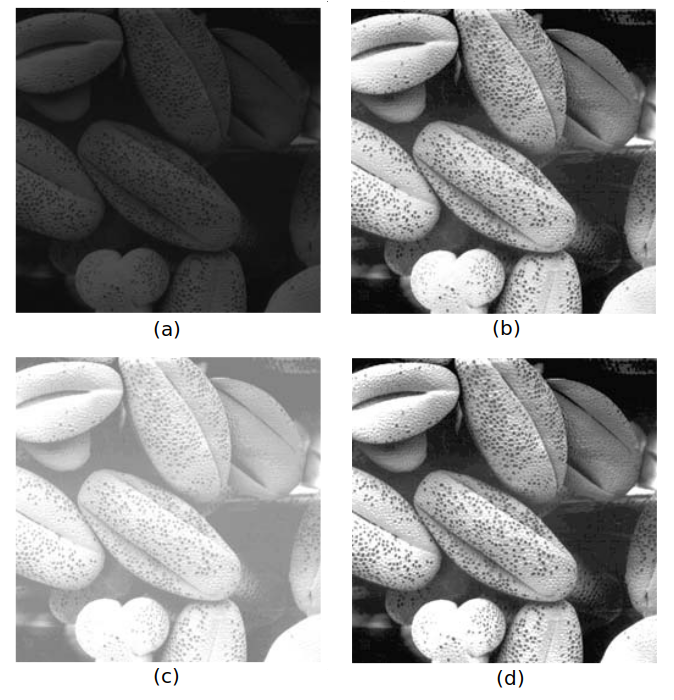
\includegraphics[scale=0.5]{images/histogram_equalization.png}
	\end{center}
	\centering
    \fadaptada{gonzalez2018digital}
\end{figure}

\subsection{Spatial Filtering}

Spatial filtering consists of the convolution of an image with a predefined kernel operator, which creates new pixel values and replaces them in the original image \cite{gonzalez2018digital}. The continuous form may be represented as a convolution over all values of a defined region of the image and the discrete form consists of sliding a weight mask over the image \cite{wu2008microscope}. Figure \ref{fig:generic_spatial_filtering} presents an arbitrary schema of a basic linear spatial filtering procedure:

\begin{figure}[htb]
	\centering
	\caption{\label{fig:generic_spatial_filtering} Arbitrary example of linear spatial filtering of an image (a) with a $3 \times 3$ filter mask (b), which results in filtered sections (c).} 
	\begin{center}
	    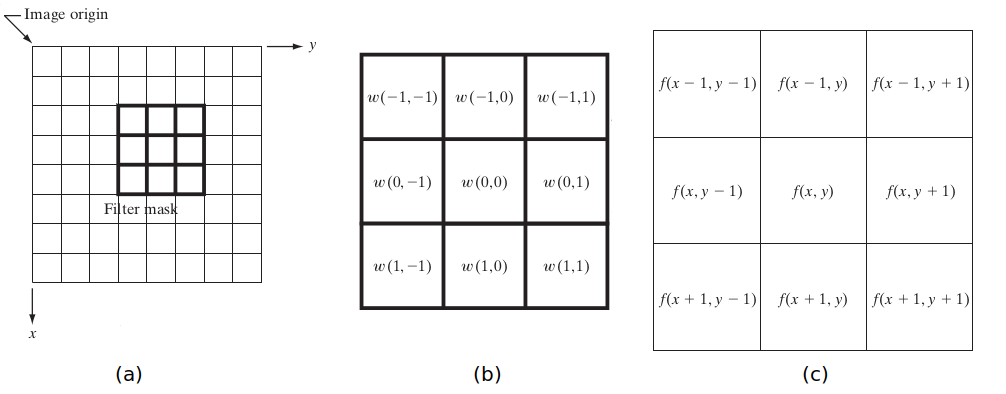
\includegraphics[scale=0.4]{images/generic_spatial_filtering.png}
	\end{center}
	\centering
    \fadaptada{gonzalez2018digital}
\end{figure}

Examples of discrete spatial filtering in digital image processing are smoothing filters, order-statistic nonlinear filters and sharpening filters, illustrated according to \cite{gonzalez2018digital}. Smoothing spatial filters are applied to remove small details, edges and lines from an image, i.e. blur, or to reduce noise. The order-statistic nonlinear filters are based on ordering pixels of the image under the filter area and replacing the pixel value in the center of the area with the response from ordering; one example is the \emph{median filter}, which replaces the center pixel with the median of pixels in its neighborhood. Median filters yield significant noise reduction effects if the nature of the noise is random. Finally, the sharpening filters are built to highlight transitions in intensity by spatial differentiation and are used for enhancing edges.

\subsection{Contrast Limited Adaptive Histogram Equalization}

Contrast enhancement may be described as the slope of the function that is relating input image intensity value to desired resultant image intensities \cite{sonali2019approach}. Histogram equalization is one of the techniques to perform contrast enhancement and works in an image by mapping the distribution of its gray levels to an approximately uniform distribution. The performance of this process is deeply related to the amount of noise in the image since it consists of peaks in the histogram, which unbalances the mapping and enhances noisy structures. One solution to this problem, according to \citeonline{zuiderveld1994constrast}, is to divide the image into \emph{contextual regions}, i.e. rectangular areas of $8 \times 8$ size, compute the optimal contrast for each of the regions and merge the results with bilinear interpolation to avoid boundary effects. This method is known as \sigla{AHE}{Adaptive Histogram Equalization}, where the global outlier gray levels do not influence each contextual region contrast enhancement.

The \sigla{CLAHE}{Contrast Limited Adaptive Histogram Equalization} method was proposed to overcome the drawback of noise. As stated by \citeonline{sonali2019approach}, it is the method that improves the low contrast issue and operates by limiting the contrast enhancement that is usually performed by ordinary histogram equalization or the AHE, which results in the noise enhancement as well. It is accomplished by allowing only a maximum number of pixels in each of the histogram bins and equally distributing the clipped pixels among the whole histogram \cite{zuiderveld1994constrast}. Figure \ref{fig:hr_ahe_clahe} presents an example of the differences between histogram equalization techniques and their results in a \sigla{MRI}{Magnetic Resonance Imaging} example:

\begin{figure}[htb]
	\caption{\label{fig:hr_ahe_clahe} MRI image of a human knee \textbf{(a)}, a simple histogram equalization \textbf{(b)}, an adaptive histogram equalization \textbf{(c)} and the contrast limited adaptive histogram equalization \textbf{(d)}.} 
	\begin{center}
	    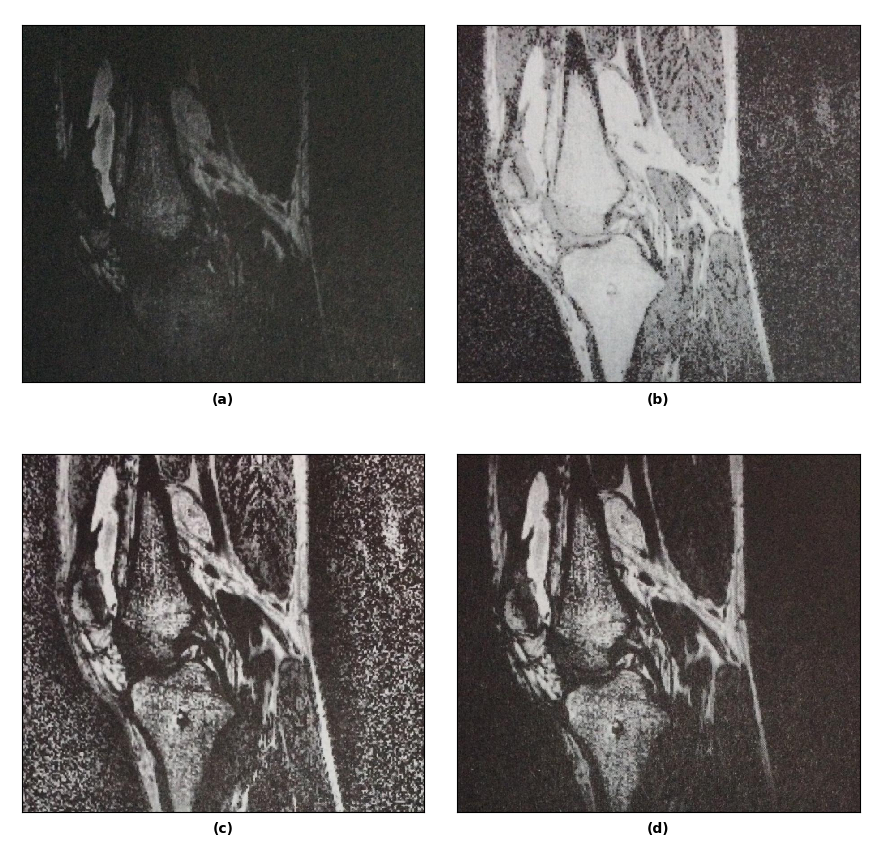
\includegraphics[scale=0.4]{images/knee_HE_AHE_CLAHE.png}
	\end{center}
	\centering
    \fadaptada{zuiderveld1994constrast}
\end{figure}


\section{Image Registration}
When a set of images of the same scene is acquired in different conditions such as distinct focus configurations, sensors or times, each image should be geometrically aligned according to a reference image if the final imaging application requires a combination of each image content. The process of overlaying two or more images with different acquisition settings is named image registration and plays an important role as a pre-processing step for image fusion, change detection and multichannel image restoration \cite{zitova2003image}. According to \citeonline{gonzalez2018digital}, magnetic resonance imaging and positron emission tomography systems, for example, are two different sensors that may acquire medical images that need to be registered; images which were taken in different times such as satellite images also need to be registered.

The image registration methods consist of the following steps, as reported by \citeonline{zitova2003image} and \citeonline{gonzalez2018digital}:

\begin{itemize}
    \item \emph{Feature detection}: the first step is to manually or automatically detect distinctive objects, e.g. edges, contours, corners and represent those as \emph{control points}, i.e. points with known locations in the reference and input images;

    \item \emph{Feature matching}: a relationship between the detected features in each image is established using feature descriptors;

    \item \emph{Transform model estimation}: this step consists of estimating parameters for mapping functions that align the input images with the reference image, either by establishing feature correspondence or performing an optimization procedure;

    \item \emph{Image resampling and transformation}: finally, the transformation occurs and the image is resampled with interpolation techniques.

\end{itemize}

Practically, the image registration is a mapping between two or more images by means of a spatial transformation and an intensity transformation \cite{brown1992survey}. Some prominent examples of registration methods are the principal axes, multiresolution, optimization-based, boundary, model-based and adaptive methods  \cite{goshtasby2012image}. The spatial transformations play an important role in all image registration techniques, and the most common general examples are rigid, affine, projective, perspective and global polynomial \cite{brown1992survey}. Still pursuant to \citeonline{brown1992survey}, each of such transformations may be described as:

\begin{itemize}
    \item \emph{Rigid}: This type of transformation accounts for object or sensor movement in which objects in the images retain their relative shape and size, and a \emph{rigid-body transformation} is an example, composed of a combination of rotation, translation, and scale change; 
    
    \item \emph{Affine}: Those are capable of tolerating more complicated distortions and preserve mathematical properties, and the \emph{shear transformation} is an example;
    
    \item \emph{Projective and Perspective}: The former deals with distortions due to projection of the objects at varying distances to the sensor onto the image plane, and the latter demands prior knowledge about the locations of the objects in the scene relative to the sensor;
    
    \item \emph{Polynomial}: Finally, the polynomial transformations can cover the broadest range of distortions, as long as those are approximately homogeneous among the image.
\end{itemize}

In the scope of this work, the microscopy images were registered with a particular combination of methods. The feature extraction was done with a custom implementation of the \sigla{SIFT}{Scale Invariant Feature Transform}, together with a custom extension of the \sigla{RANSAC}{Random Sample Consensus} method for parameter estimation and the geometric consensus filtering process with the expected transformation model and a maximal expected error as parameters \cite{saalfeld2019computational}. Those techniques will be described next.

\subsection{Scale-invariant feature transform}

As originally proposed by \citeonline{lowe1999object}, the SIFT is a feature extraction approach for object and scene recognition which consists of the following steps:

\begin{itemize}
	\item \emph{Scale-space extrema detection}: Initially, a difference-of-Gaussian function is applied in order to identify the invariant scale and orientation keypoints;
    
    \item \emph{Keypoint localization}: Each keypoint candidate is selected based on measures of their stability;
    
    \item \emph{Orientation assignment}: One ore more orientations are assigned to each keypoint location based on image gradient directions;
    
    \item \emph{Keypoint descriptor}: Finally, a measurement of the local image gradients is done for the particular scales and neighborhood of each keypoint, followed by a    transformation of those into a proper representation.
	
\end{itemize}

The custom SIFT implementation is described here as proposed by \citeonline{lowe2004distinctive}. The difference-of-Gaussian method for the detection of scale-space extrema is a convolution of an image $f(x,y)$ with the difference of two nearby scales of distance $k$, given by

\begin{equation}
\label{eqn:DoG}
D(x,y,\sigma) = \left(G(x,y,k \sigma) - G(x,y,\sigma)\right) f(x,y),
\end{equation}

\noindent where $D(x,y,\sigma)$ is the result of the convolution and $G(x,y,\sigma)$ stands for a Gaussian function described as

\begin{equation}
\label{eqn:gaussian_function}
G(x,y,\sigma) = \frac{1}{\sqrt{2 \pi \sigma}} e^{- \frac{x^{2} + y^{2}}{\sigma^{2}}}.
\end{equation}

The difference-of-Gaussians is constructed by convolving the image with several Gaussians separated by the multiplicative factor $k$, followed by a division of the scale-space by means of multiplying $\sigma$ by two at each scale change. Later, the local maxima and minima (extrema) are detected by checking around 8-neighborhoods in the current image and 9-neighborhoods within the image in adjacent scales.

With the scale-space extrema in hands, the keypoints are localized by fitting a 3D quadratic function of local sample points with the Taylor expansion

\begin{equation}
\label{eqn:taylor_DoG}
D(\mathbf{x}) = D + 
                \frac{\partial D^{T}}{\partial  \mathbf{x}}\mathbf{x} + \frac{1}{2}\mathbf{x^{T}}\frac{\partial^{2} D}{\partial \mathbf{x}^{2}}\mathbf{x},
\end{equation}

\noindent where the derivatives of the difference-of-Gaussians matrix $D$ is computed at the sample point and $\mathbf{x} = (x,y,\sigma)^{T}$ is the offset for such point. The extremum location is found with the derivative of $D$ with respect to $\mathbf{x}$ and setting it to zero. The value of $D$ at the extremum provides a way to include only stable and good contrast extrema. Together with this low contrast keypoint exclusion, it is necessary to exclude those which possess a large principal curvature across the edge direction and a small one in its perpedicular direction; this is achieved by means of a threshold based on the sum and product of the eigenvalues from the trace and determinant of a Hessian matrix computed at the location and scale of each keypoint.

The next step is to provide the orientation of each keypoint concerning local image properties. This yields invariance to image rotation and is done by computing the gradient magnitude and the orientation for each smoothed image sample, denoted by

\begin{equation}
m(x,y) = \sqrt{(L(x + 1, y) - L(x - 1, y))^{2} + (L(x, y + 1) - L(x, y - 1))^{2}}
\end{equation}

\begin{equation}
\theta(x,y) = \tan^{-1}
			\left(
			\frac{L(x, y + 1) - L(x, y - 1)}
				 {L(x + 1, y) - L(x - 1, y)}
			\right),
\end{equation}

\noindent where $m(x,y)$ is the gradient magnitude, $\theta(x,y)$ is the orientation and $L(x,y)$ is the smoothed image, i.e. the observed image convolved with a Gaussian kernel. The obtained information is sampled around each keypoint location at the selected scale and Gaussian blur level, in order to generate the descriptor representation. The samples are then weighted by a Gaussian window and accumulated into orientation histograms that represent $4 \times 4$ subregions. The descriptors are computed from a $16 \times 16$ subarray. Finally, the advantages of the custom implementation of SIFT are the invariance to image rotation and scale, robustness across a substantial range of distortions (affine, additive noise and illumination changes) and computational efficiency.

The RANSAC algorithm is a non-deterministic iterative method of fitting a mathematical model to experimental data and also an outlier detector. \cite{fischler1981random}. Concerning the image registration application in this work, it is used to identify corresponding landmark points in overlapping image tiles \cite{saalfeld2019computational}. Then, the recognized matching points in each image undergo the geometric consistency filtering process with the expected transformation model and the maximal expected error parameters; this last filtering process aims to verify if all points support the same transformation model and yield the best matches concerning all points for each image of the dataset.

\section{Image Fusion}
Image fusion is a process that merges several images, possibly acquired in diverse conditions or with different cameras, into one image with higher quality, more details and consequently more useful for humans and computer tasks \cite{mitchell2010image}. Examples of image fusion applications are noise reduction, edge enhancement, and super-resolution. One traditional use of image fusion occurs in medical imaging fields; the quality of information about illnesses, cells, clinical analysis and several other medical tasks (including the computer-assisted ones) have found profitable results from the image fusion techniques and led themselves to better and faster decisions when it comes to human beings \cite{james2014medical}. There are also relevant applications in remote sensing multispectral images, segmentation of regions in different color spaces, biometry: the pan-sharpening process is the generation of a high-resolution multispectral image from low to high-resolution ones, K-Means segmentation and fusion of pixels in the RGB and the Iris Recognition biometric process with video frames are examples of such tasks, respectively \cite{mitchell2010image}.


Also according to \citeonline{mitchell2010image}, the general framework for the image fusion procedure consists of four stages: \emph{Multiple Input Images}, \emph{Common Representational Format}, \emph{Fusion} and \emph{Display}.
The multiple input images stage is simply the acquisition of the images to be merged. There are several approaches to this: the dataset may be captured from different sensors, under distinct light conditions or angles, with different magnifications, under several focus settings, and with temporal measurements, if the scene changes through time.

If the acquired dataset images do not share the same features such as dimension, rotation angle, and resolution, then the images should be pre-processed in order to arrive at a common state. This configures the common representational format step, which generates a new and temporary dataset with the same properties, e.g. color space, dimensions, and noise level. The fusion stage employs a decision method to dictate which regions, objects, colors or details will compose the final image; some methods rely on the wavelet transform, for example. Finally, the display stage provides a view of the resulting image, which can be used directly for any further task or even be the input for other image processing operations. \autoref{fig:fusion_general_framework} depicts an arbitrary example of the four stages. 

\begin{figure}[ht]
	\centering
	\caption{\label{fig:fusion_general_framework}Image fusion general framework. (a) Multiple Input Images, (b) Common Representational Format, (c) Fusion and (d) Display.}
	\begin{center}
    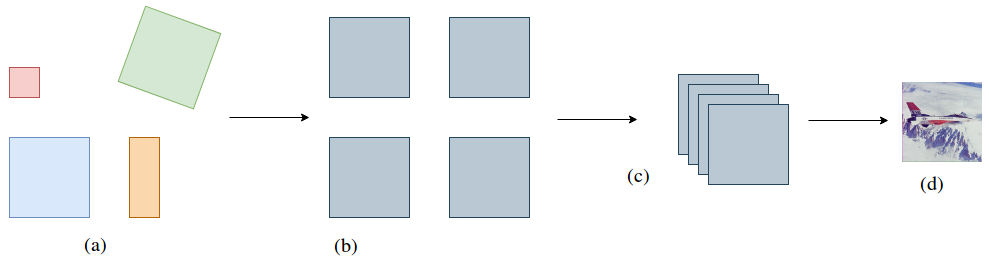
\includegraphics[scale=0.45, trim={0 -1.5cm 0cm -1.5cm}, clip]{images/image_fusion_scheme.png}
	\end{center}
	\centering
    \fautor
\end{figure}

The four arbitrary images in \autoref{fig:fusion_general_framework}.\textbf{(a)} represent different images of the same scene, taken at different resolutions, rotation angles, and shapes. In \autoref{fig:fusion_general_framework}.\textbf{(b)}, the images are all reshaped, converted to common color space and ready to undergo the processing algorithm which will transform them into feature vectors. \autoref{fig:fusion_general_framework}.\textbf{(c)} represents the image fusion by means of an arbitrary fusion rule. The resulting image is depicted in \autoref{fig:fusion_general_framework}.\textbf{(d)}. Since image fusion is only one branch of data fusion field, this procedure has a wide variety of approaches and methods; hence, the domain will be restricted to the multi-focus image fusion and some relevant related work will be presented in \autoref{chapter:related-work}.

\section{Image Quality Assessment}
\sigla{IQA}{Image Quality Assessment} is the evaluation of image quality as perceived by an average human observer, i.e. how close an image is to a given original or reference image. It is also related to the accuracy of the image acquisition process for an imaging system \cite{bovik2009essential}. It is known that images are frequently used in health and life sciences, public security systems, remote sensing, and several other fields; hence, there are computational applications that offer some useful service employing image processing. As a result, assessing image quality poses as an important task among those applications for which several techniques are being developed, evolved and deployed.

According to \citeonline{tang2019feature}, the IQA methods are distributed between the subjective assessment and objective assessment categories. The former is based on a well-defined test environment for random observers to label images and provide the final \sigla{MOS}{Mean Opinion Scores}, while the latter is based on the use of strategies such as statistical modeling, machine learning, spatial or spectral image features and so on. It is evident that subjective IQA is demanding; consequently, objective methods are preferred to conduct IQA.

According to \citeonline{wang2004image}, there are three classes of objective image quality metrics that relate to the existence of a no-distortion image (or with a negligible amount of it) for comparison purposes. The \sigla{FR-IQA}{Full-Reference Image Quality Assessment} methods assume that the reference image is available, while \sigla{RR-IQA}{Reduced-Reference Image Quality Assessment} methods employ a representation of the reference image, such as a set of extracted features. Finally, the \sigla{NR-IQA}{No-Reference Image Quality Assessment} methods, also known as ``blind'', are those which do not employ a reference image. \autoref{fig:mssim_IQA_exampe} denotes an example of a full-reference method, the \sigla{MSSIM}{Mean Structural Similarity Measure} method and its output for an image with different types of degradation:

\begin{figure}[ht]
	\centering
	\caption{\label{fig:mssim_IQA_exampe} Example of the MSSIM method output: Original image (a), contrast-stretched image (b), mean-shifted image (c), JPEG compressed image (d), blurred image (e) and salt-pepper impulsive noisy image (f).}
	\begin{center}
    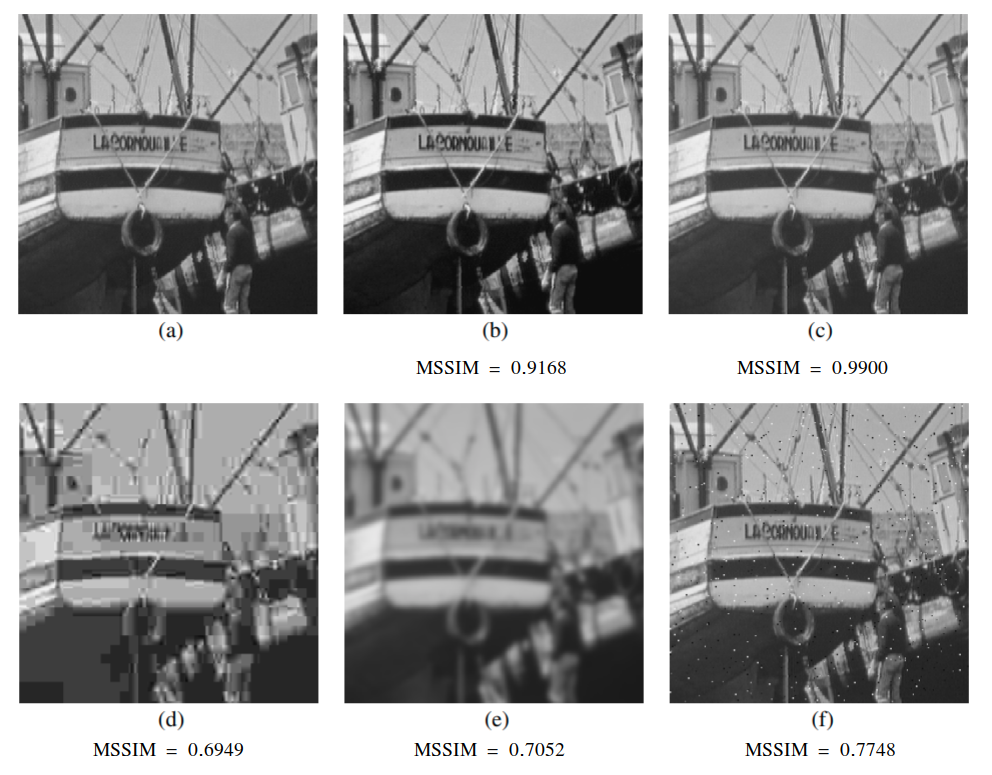
\includegraphics[scale=0.4]{images/mssim_IQA.png}
	\end{center}
	\centering
    \fdireta{wang2004image}
\end{figure}

IQA methods are also present within microscopy and its close interaction with image processing. The image acquisition in microscopy techniques may involve lasers, transmitted or reflected light, measurements of atomic force responses, the fluorescence of chemical compounds and several other means. Each technique has an inherent kind of degradation that affects the acquired images or spectra, e.g. the Raman confocal microspectroscopy suffers from the interference of cosmic rays, which yields unexpected peaks in the spectrum. Therefore, the use of IQA methods is expected. They will be investigated and used in this work. In \autoref{chapter:related-work}, some examples of NR-IQA techniques that guided the development of our method will be presented.

\section{Statistics}
Statistics is the science of planning studies and experiments, obtaining data, organizing, summarizing, presenting, analyzing, and interpreting those data and then drawing conclusions based on them; particularly among its main applications, the \emph{descriptive statistics} is a branch that comprises a set of methods which aim to describe relevant characteristics in data \cite{triola2017elementary}. The descriptive statistics methods either employ graphical elements such as boxplots, histograms, bar graphs and scatter plots to analyze data or yield numerical summary measures such as means, standard deviations, correlation coefficients and other related indices \cite{devore2011probability}. The methods that compose a descriptive statistical approach for data analysis are simple yet powerful tools that play a very important role within the scope of this project. The \emph{kurtosis} and the \emph{z-score} are the most prominent measurements for the application and will be clearly explained after some basic concepts. The graphical methods are irrelevant to this work.

Chapter~\ref{chapter:materials_and_methods} will provide information about the nature of data to be analyzed in this work. The concepts of \emph{population}, \emph{sample} and \emph{variable} are elementary: a population is a well-defined collection of objects that might be included in the analysis, a sample is a subset of a population and a variable is a feature of the objects which may change from one object to another \cite{devore2011probability}. Moreover, a \emph{frequency distribution} is a tool that presents how the data is partitioned among several categories by listing each category and its frequency of data values in each of them; a \emph{relative frequency distribution} is a frequency distribution where each frequency is represented by a proportion, usually as percentage \cite{triola2017elementary}.

\subsection{Measures of Central Tendency}

According to \citeonline{mendenhall2016statistics}, the measures of central tendency provides several ways to locate the center of the relative frequency distribution, and the three most common are the \emph{arithmetic mean}, i.e. the average of the measurements, the \emph{median}, i.e. the middle number when the measurements are ordered in ascending or descending order and the \emph{mode}, i.e. the value that occurs with the greatest frequency. Figure \ref{fig:central_tendency} presents the interpretations of these three metrics for a relative frequency distribution:

\begin{figure}[H]
	\centering
	\caption{\label{fig:central_tendency} Examples of the mean (a), median (b) and mode (c) for a relative frequency distribution.}
	\begin{center}
    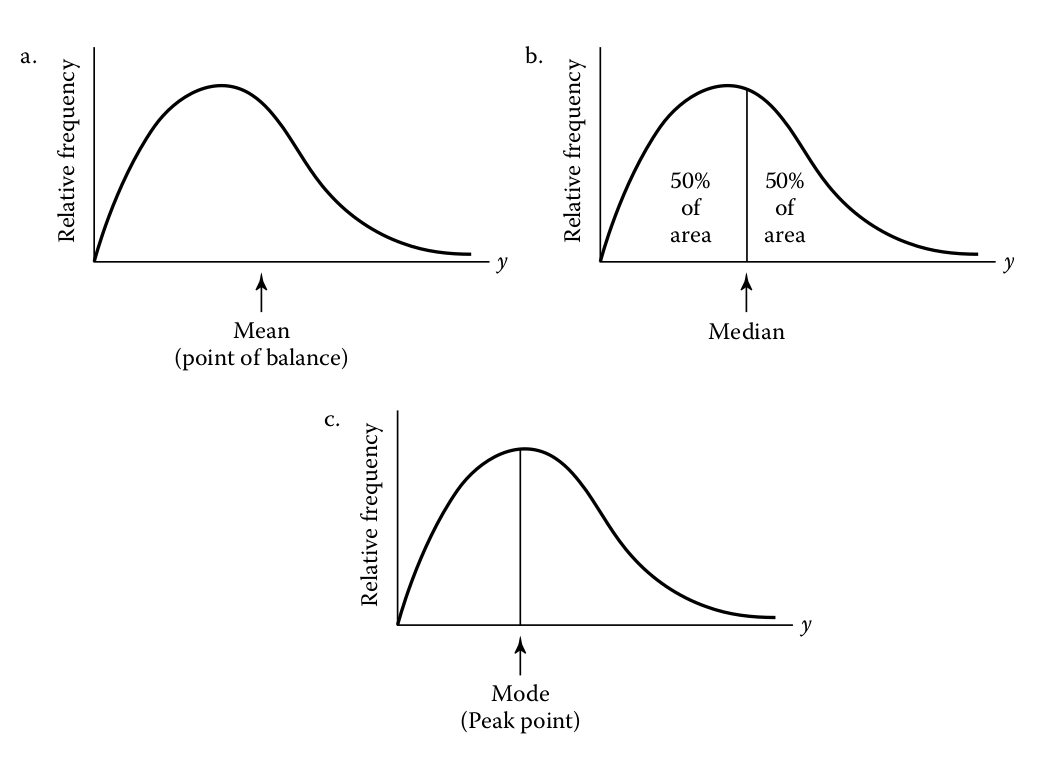
\includegraphics[scale=0.4]{images/central_tendency.png}
	\end{center}
	\centering
    \fadaptada{mendenhall2016statistics}
\end{figure}

Mathematically, the arithmetic mean is given by

\begin{equation}
\label{eqn:arithmetic_mean}
\bar{x} = \frac{1}{n} \sum_{i=1}^{n} x_{i} = \frac{x_{1} + x_{2} + \dots + x_{n}}{n},
\end{equation}

\noindent where $n$ is the sample size and $x_{i}$ represents the $i$-th observation of the variable $x$ \cite{zwillinger1999crc}.

\subsection{Measures of Variation}

The measures of variation describe how the values spread in the distribution, and commonly used measures are the range, the variance, and the standard deviation \cite{mendenhall2016statistics}. The range is simply the difference between the largest and the smallest value within the data, which may precisely point out its variability since it does not comprise the middle values among the distribution \cite{devore2011probability}. The variance measures variability based on the squared deviations about the mean and the standard deviation is the positive square root of the variance, as

\begin{align}
\label{eqn:variance_std}
\sigma^{2} = \frac{1}{n - 1} \sum_{i = 1}^{n} \left(x_{i} - \bar{x}\right)^{2}
&&
\sigma = \sqrt{\sigma^{2}},
\end{align}

\noindent where $\sigma^{2}$ and $\sigma$ are respectively the variance and the standard deviation, $x_{i}$ is the $i$-th observation of the variable $x$, $\bar{x}$ is the mean, all concerning a sample or the population \cite{zwillinger1999crc}.

\subsection{Measures of Relative Standing}

The measures of the relative standing of observations describe its locations among other values in the distribution, and two examples of these measures are \emph{percentiles} and \emph{z-scores} \cite{mendenhall2016statistics}. Percentiles are values that split the data into 100 parts in a sorted dataset, so that the $i$-th percentile stands for the $i(n + 1) / 100$ observation, e.g. the $25$-th percentile comprises $25\%$ of the data; the $z$-score, or standard score, is given by

\begin{equation}
\label{eqn:z_score}
z = \frac{x_{i} - \bar{x}}{\sigma},
\end{equation}

\noindent where $x_{i}$ is the $i$-th observation of the variable $x$, $\bar{x}$ is the mean and $\sigma$ is the standard deviation of the population or the sample \cite{zwillinger1999crc}.

\subsection{Probability Distributions}

Probability is a common and natural concept among human life, used in expressions such as ``It probably will be cold tonight''; however, there is no common formal definition accepted among statisticians and related researchers \cite{degroot2012probability}. The study of randomness, variability, and uncertainty in populations is done by analyzing probabilities, i.e. numerical descriptions of how likely an event is to occur \cite{devore2011probability}. Some basic concepts that support the probability theory are described also to the light of \citeonline{devore2011probability}, as follows:

\begin{itemize}
    \item \emph{Experiment}: Any activity or process whose outcome is subject to uncertainty;
    
    \item \emph{Sample Space}: The sample space of an experiment is the set of all possible outcomes for it;
    
    \item \emph{Event}: Any collection or subset of outcomes of a sample space;
    
    \item \emph{Random Variable}: Any rule that associates a number with each outcome in a sample space of some experiment; mathematically, it is a function with the sample space as its domain and the real numbers as its range;
    
    \item \emph{Discrete Random Variable}: A random variable with a finite set or a countably infinite sequence of possible values;
    
    \item \emph{Continuous Random Variable}: A random variable that yields zero as the probability for every possible outcome or its set of possible values is in a single interval of the real line or all numbers in a disjoint union of intervals.
    
\end{itemize}

From these concepts, it is possible to define a distribution in the scope of the probability theory. The \emph{probability distribution} is a collection of all probabilities computed from a  discrete or continuous random variable with the set of real numbers; a \emph{discrete} probability distribution is represented by the probability function itself, while a \emph{continuous} probability distribution is represented by a \sigla{p.d.f}{probability density function} \cite{mendenhall2016statistics}.

\subsection{Kurtosis}

The \emph{kurtosis} is one of the probability distribution shape statistics, which measures the extent of the peak in a distribution, i.e. its ``peakedness''; smaller absolute values indicate that the distribution tends to be uniform \cite{zwillinger1999crc}. First of all, the concepts of \emph{expectation} and \emph{moments} should be described. The expectation of a random variable (and consequently, of a distribution) is a value that summarizes its nature and is given by

\begin{align}
\label{eqn:expectation}
E(X) = \int_{-\infty}^{\infty} x p(x)dx
&&
E(X) = \sum_{x} x p(x),
\end{align}

\noindent where $x$ is each possible outcome of the random variable $X$, $p(x)$ is the probability density function for a continuous random variable (left) and the probability function for a discrete random variable (right) \cite{degroot2012probability}. Still according to \citeonline{degroot2012probability}, for a random variable $X$ and every positive $k \in \mathbb{R}$, the expectation $E(X^{k})$ is
called the $k$-th moment of $X$. The $r$-th moment may be described, according to \citeonline{zwillinger1999crc}, as

\begin{equation}
\label{eqn:rth_moment}
m_{r} = \frac{1}{n}
        \sum_{i=1}^{k}p_{i}(x_{i} - \bar{x})^{r}
\end{equation}

\noindent for every $x_{i}$ in the possible outcomes of $X$. Thus, kurtosis may be defined as the ratio of the fourth moment (equation \ref{eqn:rth_moment} with $r = 4$) by the square of the variance (also equation \ref{eqn:rth_moment} with $r = 2$), denoted by

\begin{equation}
\label{eqn:kurtosis}
g_{2} = \frac{m_{4}}{(m_{2})^{2}} - 3
\end{equation}

The $-3$ constant is due to Fischer's approach, where the kurtosis of a normal distribution is zero.

\chapter{Related Work}
\label{chapter:related-work}
This chapter presents a literature review on relevant IQA and multi-focus image fusion techniques, which guided the development of our method. The continuous search for an objective image quality assessment technique covered several strategies, such as subjective testing, statistical modeling, brain science, perceptual modeling, saliency detection, and machine learning \cite{tang2019feature}. Every strategy has advantages and trade-offs, according to the nature of the images. 

There are challenging features on the multi-focus image fusion part of our method, such as the blurring and illumination patterns, inherent to the bright-field microscopy images. The most trivial pixel-level fusion techniques are simple mathematical operations such as the average or a weighted average of gray levels; those are suitable to the task, but also deliver losses in basic image features, e.g. contrast and saturation \cite{zhang2009multifocus}. Thus, there is a demand for techniques that rely on more sophisticated tools, capable of covering multiple situations: images with different resolutions, light conditions and exposure times, for instance. Multiscale transform approaches, e.g. wavelet domain transforms are good choices and provide a very flexible framework since they depend on the chosen wavelet function \cite{pajares2004wavelet}. 

\section{Image Quality Assessment}
Defocus blur is an example among all distortions that an image may be acquainted with during its acquisition or any processing application; this implies that the resulting image will have some sort of degradation in its visual quality, and therefore justify the need of objective techniques to evaluate and predict the quality of images since the subjective ways are commonly unavailable or inconvenient \cite{wang2004image}. This section presents a literature review on no-reference IQA methods based on frequency domain analysis, human perception of blur, probabilities, local contrast levels, and gray level variability. Those methods contributed significantly to achieve and evaluate the quality of images without any reference and guided the study and development of our approach. Our method explores one of those techniques, i.e. the frequency domain analysis.

\subsection{Image sharpness measure for blurred images in frequency domain}

\citeonline{kanjar2013image} proposed a Fourier Transform based algorithm to compute an image quality measure of blurred images. This approach is an attempt to quantify sharpness because the amount of high-frequency components in a blurred image is smaller than in a sharper one. The algorithm consists of the following, where $g(x,y)$ denotes the input image of size $M \times N$:

\begin{enumerate}[label=\Roman* -]
    \item Compute the Fourier Transform representation of image $g(x,y)$, denoted here by $\hat{g}(m,n)$;
    
    \item Shift the origin of the Fourier coefficients to the center of the matrix;
    
    \item For each Fourier coefficient, compute its magnitude and assign to a matrix $A(m,n)$
    
    \begin{equation*}
        A(m,n) = \sqrt{
            [\operatorname{Re}{(\hat{g}(m,n))}]^{2}
            + [\operatorname{Im}{(\hat{g}(m,n))}]^{2}
          }
    \end{equation*}
    
    \item  Calculate the maximum value $m$ of $A(m,n)$; 
    
    \item Calculate the number $t$ of pixels in $\hat{g}$ where $\hat{g} > m /1000$;
    
    \item Calculate the image quality measure $FM = t /M.N$.
\end{enumerate}

\subsection{A no-reference perceptual blur metric}

A very simple but efficient perceptual blur metric was proposed in
\cite{marziliano2002noreference}. It is also based on the fact that high-frequency components are attenuated in a blurred image. Considering that blur affects the edges and texture regions of an image, the technique attempts to measure how scattered they are. 

First, an edge detector is applied to the luminance component of the image (equivalent to a grayscale-converted image) in order to find the vertical edges. Each row of the image is scanned for pixels corresponding to edges, and the width of each edge is computed by the difference of local extrema closest to the edge. This measure is done for each edge location, and the global blur measure is the average of all computed widths.

\subsection{A No-Reference Objective Image Sharpness Metric Based on the Notion of Just Noticeable Blur (JNB)}
\label{subsec:jnb_approach}

The authors in \cite{ferzli2009noreference} employ a psychometric model, i.e. the assignment of numerical representations to subjective tests to create a perceptual sharpness metric. The subjective tests are made concerning the \emph{Just Noticeable Blur} (JNB) concept, which is the minimum amount of perceived blurriness around an edge given a contrast higher than the limit of contrast between background and foreground that is possible to notice. 

The subjective test experiment consists in the evaluation of 27 contrast values (considering the difference between the background and the foreground grayscale values), done by 18 volunteers with normal or corrected vision, with the aim to find a particular standard deviation $\sigma_{JNB}$ of a Gaussian $7 \times 7$ mask. Each contrast value yields a normalized histogram with the volunteers' responses that are treated as the probability of detecting blur as a function of the standard deviation $\sigma$. The denoted by equation \ref{eqn:psychometric_jnb}:

\begin{equation}
\label{eqn:psychometric_jnb}
P = 1 - \exp{\left( - \left| \frac{\sigma}{\sigma_{JNB} } \right|^{\beta} \right)},
\end{equation}

\noindent where $\sigma$ is the standard deviation of the Gaussian blur filter and corresponds to the blur strength at the considered edge, $\sigma_{JNB}$ is the standard deviation corresponding to the JNB threshold. The parameters $\sigma_{JNB}$ and $\beta$ are chosen by means of a least-square fitting to approximate the probabilities $P$ with the answers from volunteers. The $\sigma_{JNB}$ value is adjusted to obtain $P = 63\%$.

First and foremost, the image is divided into blocks of dimensions $64 \times 64$. Let each block and the image be denoted by $R$ and $g$, respectively. All the blocks go through a Sobel edge detection process and are later classified as “smooth” or “edge” using a threshold. If the number of edge pixels in a block is greater than $0.2\%$ of the total number of pixels in it, then it is classified as an edge block. The smooth blocks are not processed since they are not relevant in terms of blur. Then, for each block, the horizontal edge pixels are retrieved and the width of each edge is computed. With this in hands, the perceptual blur metric for each block $R_{b}$ is described by equation 

\begin{equation}
\label{eqn:perceptual_blur_metric}
D_{R_{b}} = \left(
\sum_{e_{i} \in R_{b}}
\left|
\frac{w(e_{i})}{w_{JNB}(e_{i})}
\right|_{\beta}
\right)^{\frac{1}{\beta}},
\end{equation}

\noindent where $w_{JNB}(e_{i})$ is the JNB width relative to the contrast of block $R_{b}$ for all edges $e_{i}$. The parameter $\beta$ is empirically determined to be $3.4 \leq \beta \leq 3.8$ with median $3.6$. Thus, the general blur measure concerning the whole image corresponds to the probability of all blocks being blurred, given by

\begin{equation}
\label{eqn:p_blur}
    P_{blur}(I) = 1 - \Pi_{R_{b} \in g}
    \left(
    1 - P_{blur}(R_{b})
    \right),
\end{equation}

\noindent where $P_{blur}(R_{b})$ may be substituted by $1 - \exp{\left(-D_{R_{b}}^{\beta} \right)}$, which results in

\begin{align}
\label{eqn:p_blur_final}
    P_{blur}(I) = 1 - \exp{\left(-D^{\beta}\right)}
&&
D = \left(
    \sum_{R_{b}}
    \left|D_{R_{b}}
    \right|^{\beta}
    \right)^{\frac{1}{\beta}}.
\end{align}

\noindent Finally, $D$ from equation \ref{eqn:p_blur_final} is then normalized by the amount of blocks an represents the final image quality index.

\subsection{A No-Reference Image Blur Metric Based on the Cumulative Probability of Blur Detection (CPBD)}

A sharpness metric that extends the approach described in \ref{subsec:jnb_approach} was proposed in \cite{narvekar2011noreference}. It is based on the cumulative probability of blur detection (CPBD), which applies the same psychometric function framework from JNB. The $w_{JNB}$ value is defined as 5 if the contrast is less or equal to 50 and 3 otherwise. The metric explores the normalized histogram of the probability of blur detection from the whole image, where CPBD is the percentage of edges at which blur is not likely to be detected.

First, the horizontal edges from the image are detected, also divided into blocks of $64 \times 64$ and classified as edge blocks or sharp blocks with the same threshold as in \citeonline{ferzli2009noreference}. The probability of detection blur for and edge $e_{i}$ is computed with the equation \ref{eqn:cpbd_jnb}

\begin{equation}
\label{eqn:cpbd_jnb}
\begin{split}
    P_{BLUR} &= P_{BLUR}(e_{i})\\
    &= 1 - \exp{
    \left(
        - \left|
            \frac{w(e_{i}}{w_{JNB}(e_{i})}
        \right|^\beta
    \right)}.
\end{split}
\end{equation}

\noindent Then, the cumulative probability of blur detection is computed from the probability density function of equation \ref{eqn:cpbd_jnb}, and may be described as

\begin{equation}
\label{eqn:cpbd}
\begin{split}
    CPBD &= P(P_{BLUR} \leq P_{JNB})\\
    &=\sum_{P_{BLUR} = 0}^{P_{BLUR} = P_{JNB}}P(P_{BLUR}).
\end{split}
\end{equation}

\noindent Thus, greater values for the CPBD metric mean sharper images.


\subsection{S3: A Spectral and Spatial Measure of Local Perceived Sharpness in Natural Images}

\citeonline{vu2012s3} proposed one technique to assess image quality that explores both spatial and spectral information from the image. The denomination $S_{3}$ represents the combination of $S_{1}$, which denotes the spectral measure of sharpness and $S_{2}$, which the authors denote as the spatial measure of sharpness. The first step is to convert the RGB image to the grayscale color space with weights $0.2989$, $0.5870$ and $0.1140$ for the red, green and blue channels, respectively. The grayscale image is then divided into blocks denoted by $\mathbf{x}$ of dimensions $m \times m$ and an overlap $d$ around each neighbor block.

In order to compute the $S_{1}(\mathbf{x})$ measure, the first step is to compute the luminance contrast of each $\mathbf{x}$ block, denoted by $CR$ with the equation

\begin{align}
\label{eqn:luminance_contrast}
CR(\mathbf{x}) = l(\mathbf{x}) = \left(b + k\mathbf{x}\right)^{\gamma}
&&
b = 0.7656;\; k = 0.0364;\; \gamma = 2.2
\end{align}

\begin{align*}
\label{eqn:contrast_constraints}
CR(\mathbf{x}) = 0 \iff
    \begin{cases}
        max(l(\mathbf{x})) - min(l(x)) \leq T_{1}\\
        \mu_{1} \leq T_{2}    
    \end{cases}
&&
T_{1} = 5;\; T_{2}= 2.
\end{align*}

\vspace{0.1in}

\noindent The $S_{1}$ measure for a block is set to zero if the contrast is zero. For the blocks with $CR > 0$, the magnitude spectrum is computed from the two-dimensional DFT, which is defined as the modulus of each complex coefficient and represents how much each frequency is present in the image and is represented here as $mag(\hat{\mathbf{x}})$. Then, the slope of the magnitude spectrum denoted by $\alpha_{\mathbf{x}}$ is the slope of a line in the standard form $ax + b$ and is obtained by linear regression with

\begin{equation}
\label{eqn:slope_of_magnitude}
\alpha_{\mathbf{x}} = \arg \min_{\alpha} \left\lVert \beta \hat{\mathbf{x}}^{-\alpha} -  mag(\hat{\mathbf{x}}) \right\rVert^{2}_{2},
\end{equation}

\noindent where the $L_{2}$ norm is taken over all frequencies. From this framework, $S_{1}(\mathbf{x})$ is described by

\begin{equation}
\label{eqn:sigmoid_s1}
S_{1}(\mathbf{x}) = 1 - \frac{1}{1 + e^{\tau_{1}
(\alpha_{\mathbf{x}} - \tau_{2})}},
\end{equation}

\noindent where $\tau_{1} = -3$ and $\tau_{2} = 2$. Equation \ref{eqn:sigmoid_s1} is a sigmoid function to estimate sharpness considering the slope of the spectral magnitude. This measure does not include the contrast information directly and it may generate inaccurate classifications; this is the reason why the authors propose the use of spatial information.

$S_{2}$ incorporates the spatial information by analyzing the 8-neighborhoods of pixels in a block $\mathbf{x}$. The \sigla{TV}{Total Variation} is a metric of regularity within the grayscale values and is mathematically described as

\begin{equation}
\label{eqn:total_variation}
v(\mathbf{x}) = \frac{1}{255}\sum_{i,j}\left|x_{i} - x_{j}\right|,
\end{equation}

\noindent where $x_{i}$ and $x_{j}$ are 8-neighbors in $\mathbf{x}$. The TV provides a good representation of the absolute differences in each block; this implies that the contrast information is consequently described well. The larger the TV index is, the higher the contrast in the block. The $S_{2}$ map is then computed as

\begin{equation}
\label{eqn:spatial_s2}
S_{2} = \frac{1}{4} \max_{a \in \mathbf{x}} v(a),
\end{equation}

\noindent where $a$ is a $2 \times 2$ block of $\mathbf{x}$. Each $x$ is of dimensions $8 \times 8$ and the overlap is $d = 4$. The final map for the whole image is the sum of all indices for each of the blocks.

Finally, let $\mathbf{X}$ denote the set of all blocks which form the image. The $S_{3}$ image quality index is the weighted geometric mean defined by

\begin{equation}
\label{eqn:s3_index}
S_{3}(\mathbf{X}) = S_{1}(\mathbf{X})^{\eta} S_{2}(\mathbf{X})^{1 - \eta},
\end{equation}

\noindent where $0 \leq \eta \leq 1$, and $\eta = 0.5$ is the best empirically obtained value for the parameter.

\subsection{A Fast Approach for No-Reference Image Sharpness Assessment Based on Maximum Local Variation}

\citeonline{bahrami2014fast} proposed the \sigla{MLV}{Maximum Local Variation} metric for image sharpness assessment. The MLV metric improves the idea of the total variation measure. Instead of computing the variations of pixel values among 8-neighborhoods, the authors propose the maximum among all differences in a neighborhood, represented by $\psi$ described by

\begin{align}
\label{eqn:mlv}
\psi(g(i,j)) = \max(g(i,j) - g(k,l))
&&
x = \{i - 1, i, i + 1\};\;\;
y = \{j - 1, j, j + 1\},
\end{align}

\noindent where $g(k,l)$ with the bounds for $k$ and $l$ denoted in equation \ref{eqn:mlv} are the 8-neighbors of the pixel $g(i,j)$. In a nutshell, the metric finds the maximum among the 8-neighborhood of a pixel, concerning the $\ell_{1}$ norm as a distance. With this setup, the algorithm begins with the grayscale conversion of an image of dimensions $M \times N$. The neighborhoods are $3 \times 3$ blocks along the image and the MLV is computed for all pixels, which results in a map $\Psi(g)$ given by

\begin{equation}
\label{eqn:mlv_matrix}
\Psi(g) =
    \begin{pmatrix}
        \psi(g(1,1)) & \cdots &  \psi(g(1,N))\\
        \vdots & \ddots & \vdots\\
        \psi(g(M,1)) & \cdots & \psi(g(M,N)).
    \end{pmatrix}
\end{equation}

\noindent The next step is to apply a statistical technique to analyze how the distribution of $\Psi$ behaves when the image is sharp or blurred. For the sharp regions, i.e. high MLV values or black content, the distribution is closer to hyper-laplacian; for smoother and blurred regions, the distribution is closer to Gaussian. Therefore, the authors chose to parametrize the MLV with a \sigla{GGD}{Generalized Gaussian Distribution}, which covers the Gaussian, the laplacian and hyper-laplacian distributions and is denoted as

\begin{equation}
\label{eqn:GGD_distribution}
GGD(\Psi(g); \mu, \gamma, \sigma) =
\left(
    \frac{\gamma}{2 \sigma \Gamma \left( \frac{1}{\gamma} \right) \sqrt{\frac{\Gamma \left( \frac{1}{\gamma} \right)}{\Gamma \left( \frac{3}{\gamma} \right)}}}
\right)
e^{- \left(
        \frac{\Psi(g) - \mu}{\sigma \sqrt{\frac{\Gamma \left( \frac{1}{\gamma} \right)}{\Gamma \left( \frac{3}{\gamma} \right)}}}
    \right)^{\gamma}},
\end{equation}

\noindent where $\mu$ is the mean, $\sigma$ is the standard deviation, $\gamma$ is the shape parameter and $\Gamma$ is the gamma function. In a nutshell, the MLV metric is relative to the standard deviation of the GGD distribution: the sharper the image is, the higher the standard deviation. The $\Psi$ matrix is weighted with values obtained with the exponential function $w_{i,j} = e^{\eta_{i,j}}$, where $\eta_{i,j}$ is the rank of $\psi(g(i,j))$ when sorted in ascending order.

\section{Multi-focus Image Fusion}
Either in microscopic or macroscopic scales, imaging devices have a finite depth of field. Blurry regions in images may occur due to several reasons, e.g. the acquisition outside the boundaries of depth of field \cite{huang2007evaluation}. Therefore, it is nearly impossible to obtain a globally sharp image in microscopic scales, since height differences within the surface of the sample will also be magnified and the depth of field of microscopes is usually small. Image fusion of stack of images, acquired with a variety of focus adjustments, may yield a fully sharp image. In this section, we investigate multifocus image fusion techniques based on principal component analysis, guided filtering with local linear models, gradients and singular value decomposition. Similarly to the proposed IQA method, our image fusion approach explores one of the well-known literature methods, i.e. a gradient-based analysis to distinguish sharp and blurry regions.

\subsection{Pixel-level image fusion using wavelets and principal component analysis}

\citeonline{naidu2008pixel} addressed the multifocus image fusion problem with two fusion rules, based on \sigla{PCA}{Principal Component Analysis} and the \sigla{DWT}{Discrete Wavelet Transform}. The Principal Component Analysis is a mathematical procedure based on linear algebra, which performs the extraction of uncorrelated variables that represent data. In other words, the PCA based fusion rule composes the image from the most relevant subset of data from each input image. The proposed PCA-based image fusion algorithm consists of the following steps:

\begin{enumerate}[label=\Roman* -]
    \item First and foremost, reshape the input images as two-column vectors, which yields a matrix of dimensions $2 \times n$, with $n$ as the original dimension of each image. Let the resulting matrix be denoted as $Z$;
    
    \item Compute the empirical mean vector of dimensions $1 \times 2$, i.e. a vector that contains the mean of observations for each variable;
    
    \item Subtract the empirical mean vector from each column of $Z$, which results in a matrix of dimensions $2 \times n$. Let the resulting matrix be denoted as $Y$;
    
    \item Compute the covariance matrix of $Y$, i.e. $YY^{T}$;
    
    \item Compute the eigenvectors and the eigenvalues of the covariance matrix and sort them by descending order. Let the eigenvectors and the eigenvalues be denoted by $V$ and $D$, respectively. Both $V$ and $D$ dimensions are $2 \times 2$;
    
    \item Compute the principal components $P_{1}$ and $P_{2}$ with the first column of $V$, as
    
    \begin{align}
    P_{1} = \frac{V(1)}{\sum V}
    &&
    P_{2} = \frac{V(2)}{\sum V}.
    \end{align}
\end{enumerate}

\noindent Finally, the fused image is composed by

\begin{equation}
g_{fused}(x,y) = P_{1}g_{1}(x,y) + P_{2}g_{2}(x,y),
\end{equation}

\noindent where $g_{fused}$ represents the fused image and $g_{1}$ and $g_{2}$ represent the input images, respectively. The process may be extended to several images by applying the method in the first two images of the dataset, then with the fused image and another image and so on.

Along with PCA, the authors explored a fusion approach with the DWT. The transform is applied to the input images and decomposes them into subbands of detailed and approximation wavelet coefficients, i.e. high and low frequency components, respectively. Finally, the fusion rule consists of averaging the approximation coefficients and choosing the maximum among each detailed coefficient in each subband.

\subsection{Image fusion with guided filtering}

The guided filtering, i.e. a windowed linear transform of the input image where coefficients are obtained by linear ridge regression was applied to perform image fusion \cite{li2013image}. The authors proposed a pixel-level image fusion technique that also make use of low pass filtering, edge extraction and spatial consistency. It consists of three steps: two-scale image decomposition, weight map construction with guided filtering and two-scale image reconstruction.

The decomposition step transform the input images into two-scale representations by means of a convolution with an average filter of size $31 \times 31$. The first representation is named \emph{base} layer, directly obtained from the average filter convolution, and the second representation is named \emph{detail} layer, obtained by subtracting the base layer from the input image.

In order to retrieve the weight map, i.e. a characterization of sharp and blurry regions of the image, an edge extraction is performed by means of Laplacian filtering with a $3 \times 3$ kernel (which will be further explained in Chapter~\ref{chapter:materials-and-methods}); subsequently, the edges undergo a Gaussian low-pass filter of dimensions $11 \times 11$ and $\sigma = 5$. Let $S_{i}^{k}$ be the smoothed edge in the pixel $k$ of the $i$th input image. The weight map is built as

\begin{equation}
\label{eqn:weight_map}
P_{i}^{k} = 
    \begin{cases}
        1, & \text{if } S_{i}^{k} = \max{(S_{1}^{k},S_{2}^{k},\dots,S_{n}^{k})}\\
        0, & \text{otherwise}
    \end{cases},
\end{equation}

\noindent where $n$ is the number of input images. The guided filter is then applied to the each image, together with its weight map, which produces final weight matrices $W_{i}^{B}$ and $W_{i}^{D}$ for the base and detail layers of each image, respectively. Subsequently, all base and detail layers are fused by means of weighted averaging with their respective weight matrices, given by

\begin{align}
\bar{B} = \sum_{i=1}^{n}W_{i}^{B}B_{i}
&&
\bar{D} = \sum_{i=1}^{n}W_{i}^{D}D_{i},
\end{align}

\noindent where $\bar{B}$ and $\bar{D}$ are the fused base and detail layers, respectively. The fused image is finally constructed by summing the fused layers.

\subsection{Multi-scale weighted gradient-based fusion for multi-focus images}

Another way to perform edge-detection based image fusion is to extract gradients from each image among a set and merge them with the structure tensor, as proposed by \citeonline{zhou2014multi}. The first processing step in this approach is to locally obtain the gradients of each input image in the form of a structure tensor, i.e. a non-negative second moment matrix where its eigenvalues represent the intensity changes in a given point, and then a local gradient covariance matrix, described as

\begin{equation}
C_{\sigma} =
    \begin{pmatrix}
        \nabla_{x}^{2} \ast G_{\sigma}
        &
        \left(
            \nabla_{x}\nabla_{y} \ast G_{\sigma}
        \right)
        \\
        \left(
            \nabla_{x}\nabla_{y} \ast G_{\sigma}
        \right)
        &
        \nabla_{x}^{2} \ast G_{\sigma}
    \end{pmatrix},
\end{equation}

\noindent where $G_{\sigma}$ is a Gaussian filter, $\nabla_{x}$ and $\nabla_{y}$ are the gradients of the image along $x$ and $y$ directions in a given pixel. The $\sigma$ parameter represents the standard deviation of the Gaussian function and also the scale of the matrix $C_{\sigma}$. The local image structure is related to the eigenvalues of $C_{\sigma}$, $s_{1}^{2}$ and $s_{2}^{2}$. Let $s_{1}$ and $s_{2}$ be the square root of such eigenvalues. If one of those is large and the other is small, it means that the pixel consists of an edge; if both are large, then the region is sharp, which indicates a corner. Then, the authors define a structure saliency measure for the image at a selected scale, as

\begin{equation}
\label{eqn:structure_saliency}
Q = \sqrt{(s_{1} + s_{2})^{2} + \alpha(s_{1} - s_{2})^{2}},
\end{equation}

\noindent where $\alpha > -1$. This is used as a sharpness measure for the multifocus images at different scales in presence of anisotropic blur and also misregistration. The sharpness is first computed at a large scale, i.e. a large $\sigma$ value, which roughly detects the focused region of each input image.

With a coarse representation of the focused regions in hands, the next step is to define an unknown region near the boundaries of each focused region and set the gradient weights as $1$ for sharp and $0$ for blurry. The gradient weights are then calculated by applying the focus measure with a small $\sigma$ value, and then merged with the gradients. This results in a set of probabilities for each pixel in each image. The composition of the fused image is then guided by the largest probability values.

\subsection{Image fusion technique using multi-resolution singular value decomposition}

\citeonline{naidu2011image} proposed a fusion technique which is similar to the DWT-based ones, but employs a Multiresolution \sigla{SVD}{Singular Value Decomposition} instead. The multiresolution SVD performs a factorization of a matrix into eigenvalues and eigenvectors in different scales by the following steps:

\begin{enumerate}[label=\Roman* -]
    \item Let $X = [x_{1},x_{2},\dots,x_{n}]$ be an one-dimensional signal of length $n$. Reshape $X$ onto a matrix given by 
    
    \begin{equation*}
        X_{1} = \begin{bmatrix}
                x_{1} & x_{3} & \dots & x_{n-1} \\
                x_{2} & x_{4} & \dots & x_{n}
                \end{bmatrix}
    \end{equation*}
    
    and a scatter matrix $T_{1} = X_{1}X_{1}^{T}$;
    
    \item Factorize the matrix $T_{1}$. Let the eigenvector matrix of $T_{1}$ be $U_{1}$. Then $T_{1}$ is transformed into a diagonal matrix $S_{1}^{2}$ as
    
    \begin{equation*}
        S_{1}^{2} = U_{1}^{T}T_{1}U_{1} =
        \begin{bmatrix}
            s_{1}^{2} & 0\\
            0 & s_{2}^{2}
        \end{bmatrix},
    \end{equation*}
    
    where $s_{1}^{2}$ and $s_{2}^{2}$ are the squares of the singular values. Then, let $\hat{X}_{1} = U_{1}^{T}X_{1}$. The top row of $\hat{X}_{1}$ contains the approximation component, i.e. the largest eigenvalue, and the bottom row contains the detail component, i.e. the smallest eigenvalue. Let $\varphi$ and $\psi$ represent the top and bottom rows of $\hat{X}_{1}$, respectively;
    
    \item In order to perform the image decomposition in other scales, the approximation component $\varphi$ plays the role of $X$.

\end{enumerate}

The MSVD is then a decomposition of $2 \times 2$ blocks of the image, rearranged into one-dimensional vectors of dimensions $4 \times 1$. The authors proposed a two-level decomposition, which generates 8 images from each input image. At each level, the largest absolute value among the MSVD detailed coefficients will compose the fused image, while at the coarsest level, the average of all approximation is computed and added to the output.

\chapter{Materials and Methods}
\label{chapter:materials-and-methods}
In \autoref{chapter:related-work}, the literature review showed that both no-reference image quality analysis and image fusion were addressed by many known techniques such as multiresolution analysis and principal component analysis; on the other hand, applications still evolve as new strategies such as machine learning are presented. The idea that motivated the use of the Fourier Transform as the basis for an IQA method is that it is a fast, robust and reliable analysis tool and could produce relevant results if properly explored. Similarly, the image fusion process was developed by exploring many state-of-the-art fusion applications and addressing both computational requirements (both hardware and software) and computational performance, since the method is built to work on normal optical microscope workstations instead of large clusters. As a result, we studied the capabilities of the Laplacian of Gaussian as the basis for our image fusion algorithm. 

This chapter presents all the details about our no-reference image quality assessment method and our multifocus image fusion method, as well as relevant information about the proposed datasets, including acquisition details and issues. We also show how the methods relate to each other since it also requires the human knowledge to select the images for registration and posterior fusion, similar to most of the z-stacking systems on microscopy software packages.

\section{Overview}
Our approach consists of three parts: a) an image acquisition process based on the z-stacking technique; b) a method for assessing the quality of images that explores frequency domain features and basic statistical analysis tools and outputs a quantitative index that allows the selection of focused images and c) an image fusion procedure, based on the Laplacian of Gaussian filter and energy of edges, which forms the final image. Figure~\ref{fig:overview} graphically summarizes the processing steps, which will be describe in this Chapter. Figure~\ref{fig:overview}.(a) denotes the image acquisition process, which consists of collecting specimens of plants, acquiring images with microscopes and organizing the datasets. Then the images undergo our IQA method in Figure~\ref{fig:overview}.(b), and a subset of the images is selected for registration by means of statistical methods. Finally, Figure~\ref{fig:overview}.(c) represents the image fusion procedure, which aims to produce a high-quality image.

\begin{figure}[ht]
  \centering
  \caption{Overview of each stage of our approach: \textbf{(a)} image acquisition and registration, \textbf{(b)} selection of images after IQA and \textbf{(c)} image fusion.}
  \label{fig:overview}
  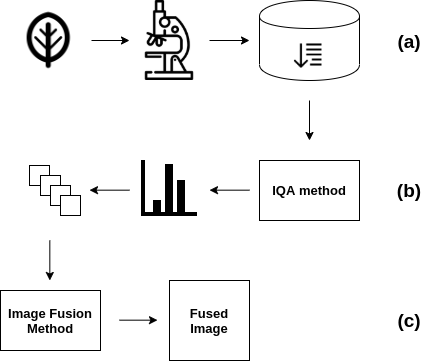
\includegraphics[scale=0.8]{images/overview.png}
  \centering
  \fautor
\end{figure}

\section{Image Datasets}
\section{Proposed dataset}

Three bright-field microscopy images datasets were acquired with the ZEISS Axiocam ERc5s camera in the ZEISS SteREO Discovery.v20 and the ZEISS AxioLab A1 stereo microscopes from the Scientific Computing Group (SCG) at São Carlos Institute of Physics (IFSC). The datasets contain images from leaf histological samples of the plants \textit{Callisia repens}, \textit{Tradescantia zebrina} and \textit{Cthenante oppenheimiana}, acquired with different focal planes and with different magnification levels. 

A shared feature among the species \textit{Callisia repens}, \textit{Tradescantia zebrina} and \textit{Cthenante oppenheimiana} is the purple abaxial (lower or bottom) leaf surface. This is commonly observed in deeply-shaded understorey plants and can be either transient or permanent, depending on the species and environmental conditions \cite{filho2018plants}. Several research projects have been conducted by the SCG group on plant leaf images, including biological studies with complex network analysis, where the locations of particular structures of the leaf, i.e. the stomata, were modeled as graphs. The \emph{stoma} (plural \emph{stomata}) is a structure that consists of an aperture between two cells, named \emph{guard cells}, and controls the exchange of steam, CO$_{2}$ and other gases from the inner part of the leaf and the atmosphere  \cite{hetherington2003role}. Furthermore, the concentration of stomata in leaves of purple plants is high; such stomatal cells are green and create a contrast between the epidermis and the stomata, which yields very good results with optical microscopy imaging \cite{filho2018plants}. Samples of blurred and sharp images of both datasets are shown in \autoref{fig:datasets}.

\begin{figure}[ht]
	\centering
	\caption{Examples of the proposed dataset images: blurred \textit{Callisia} \textbf{(a)}, sharp \textit{Callisia} \textbf{(b)}, blurred \textit{Tradescantia} \textbf{(c)}, sharp \textit{Tradescantia} \textbf{(d)} and blurred \textit{Cthenante} \textbf{(e)}, sharp \textit{Cthenante} \textbf{(f)}.}
	\label{fig:datasets}
	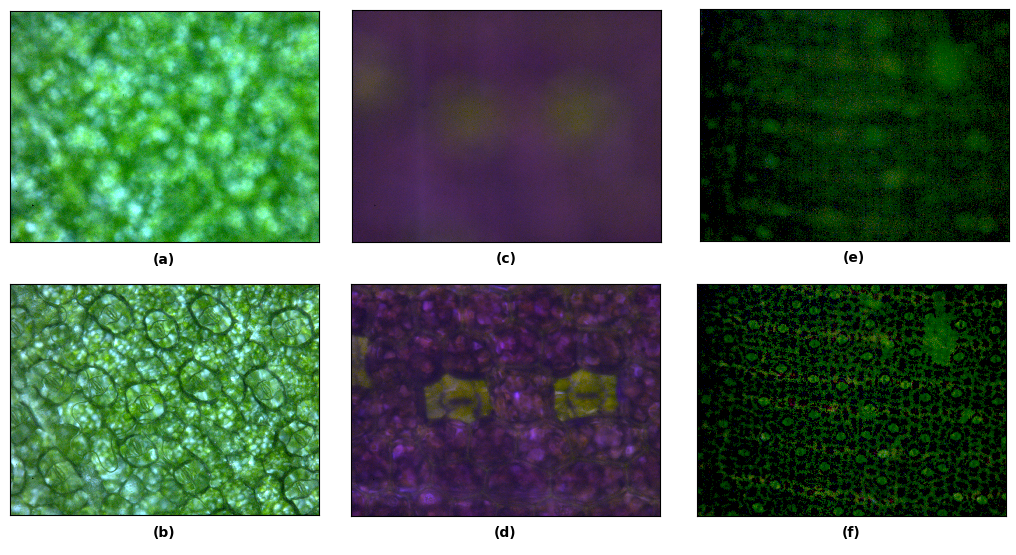
\includegraphics[scale=0.4]{images/datasets.png}
	\centering
	\fautor
\end{figure}

\subsection{Acquisition and Usage Protocols}

We will refer to the datasets as \textit{Callisia}, \textit{Tradescantia} and \textit{Cthenante} for notation simplicity. The \textit{Callisia} and \textit{Tradescantia} datasets were acquired with the z-stacking method in the SteREO Discovery.v20 microscope, whereas the \textit{Cthenante} dataset was acquired with the AxioLab A1 microscope. The workstation was connected to the microscopes by means of the ZEISS Axiovision version 4.8 software package. The z-stacks were manually built, i.e. the axial location of the objective was manually changed.

The SteREO Discovery.v20 microscope allows a precise measurement of the objective height, and the slices were acquired with a distance of 10 $\mu$m between each other - the maximum manually achievable distance. For both microscopes, the acquisition started with the objective height above the focal plane and, therefore, a completely blurred image. Then, the objective was progressively lowered in the $z$ axis, and at each step, an image was taken; this process was done until the objective height was below the focal plane and the images were blurred again.

The z-stacks were registered for image fusion after the eligible images in each set were chosen. Therefore, after the IQA method was applied, each set of eligible images was aligned with the TrakEM2 package, an ImageJ-based tool for processing and analyzing microscopy images. It includes methods for lens distortion correction, stitching, serial section alignment, correction of section thickness, and contrast adjustment \cite{saalfeld2019computational}. TrakEM2 uses  a particular combination of methods. The feature extraction was done with a custom implementation of the \sigla{SIFT}{Scale Invariant Feature Transform}, together with a custom extension of the \sigla{RANSAC}{Random Sample Consensus} method for parameter estimation and the geometric consensus filtering process with the expected transformation model and a maximal expected error as parameters \cite{saalfeld2019computational}. 

Primarily, a subjective quality index based on the Mean Opinion Score (MOS) was built in order to validate the results. The mean opinion score is the average of values on a predefined scale that an observer assigns to his opinion about the performance of a system (in this case, the imaging system) across a sample of observers \cite{liu2019comprehensive}. Practically, it consists of integer numbers in the interval $[1,5]$ where 1 is the worst score and 5 is the best. With the output of three people - two microscopy experts and one from a non-microscopy field - a subjective index was created. Most of the images were classified as 1 and the maximum score was 3. The images were then labeled as 3 - \emph{eligible} and 1 or 2 - \emph{negligible} for the fusion process, respectively. The axial nature of the acquisition allowed for a contiguous set of eligible images in each dataset. \autoref{tab:dataset_info} presents some relevant properties of each dataset.

\begin{table}[ht]
    \centering
    \caption{Information about the proposed datasets.}
    \label{tab:dataset_info}
    \begin{tabular}{lccc}
        \toprule
        \textbf{Dataset} & \textbf{\textit{Callisia}} &
        \textbf{\textit{Tradescantia}} &
        \textbf{\textit{Cthenante}}\\
        \midrule
        \textit{Magnification} & 50x & 200x & 100x\\
        \textit{Step} & 10$\mu$m & 10$\mu$m & 4$\mu$m\\
        \textit{Number of images} & 56 & 66 & 55\\
        \textit{Eligible} & 9 & 2 & 16\\
        \textit{Sharp sequence} & 41 - 49 & 50 - 51 & 30 - 45\\
        \bottomrule
    \end{tabular}
    \centering
    \fautor
\end{table}

In order to use the proposed datasets for evaluation of new methods, it is necessary to take into account that several images are totally blurred, and an image quality assessment algorithm should yield a low metric number for such images. As the $z$ position approaches the optimal focal plane, the metric may start to produce better values. The images are named with the step of the $z$-stack starting at 1, so that the eligible images are easily located. The metric should yield the highest quality values are among the range of eligible images, depicted as 
``Sharp sequence'' in \autoref{tab:dataset_info}. When the axial position is not exceeds the limits of the sharp sequence, the metric values should decay. The datasets are capable of assessing the monotonicity, accuracy and precision of image quality metrics.

\section{Benchmark datasets}

Benchmark datasets are fundamental in computer vision and image processing research in order to track the performance, accuracy and efficiency of new methods and algorithms. The image quality assessment was also evaluated against literature methods with the well-known Computational and Subjective Image Quality database (CSIQ) image quality assessment database \cite{larson2010most} and the KonIQ database, the largest image quality assessment database to date \cite{hosu2020koniq}. 

The CSIQ database contains 30 original images of dimensions $512 \times 512$. Each image is distorted in four to five different levels separately by JPEG and JPEG-2000 compression, Gaussian blurring, global contrast decrements and additive pink Gaussian noise. The Gaussian blur subset with 150 images was employed in the proposed analysis. The dataset also contains 5000 subjective rates done by 35 different observers, By means of a MOS index. 

The KonIQ database was built in order to evaluate the performance of a deep learning method for blind image quality assessment. It consists of 10073 images of dimensions $1024 \times 768$ with different labels for brightness, contrast, colorfulness and sharpness. The labels were generated from 1.2 million MOS rating of 1459 observers. One dissimilar feature of KonIQ when compared to CSIQ is that the quality assessment should be done among different scenes with different levels of degradation. \autoref{fig:csiq_example} shows two samples of the CSIQ database, and \autoref{fig:koniq_example} presents both blurred and sharp samples from the KonIQ image.

\begin{figure}[htb]
    \centering
    \caption{Samples from the CSIQ database: blurred image (a) and sharp image (b).}
    \label{fig:csiq_example}
    \begin{subfigure}[t]{0.45\textwidth}
        \centering
        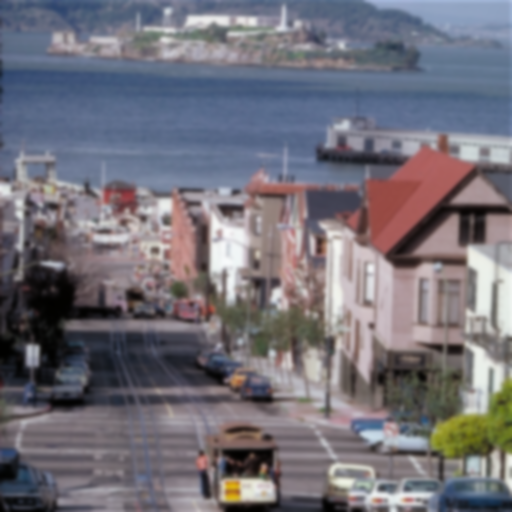
\includegraphics[height=5cm]{images/csiq_blurred.png}
        \caption{}
    \end{subfigure}%
    ~ 
    \begin{subfigure}[t]{0.5\textwidth}
        \centering
        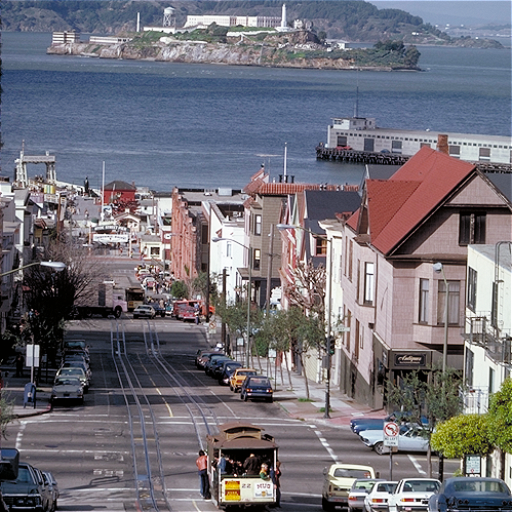
\includegraphics[height=5cm]{images/csiq_sharp.png}
        \caption{}
    \end{subfigure}
    \centering
    \fdireta{larson2010most}
\end{figure}

\begin{figure}[htb]
    \centering
    \caption{Samples from the KonIQ database: blurred image (a) and sharp image (b).}
    \label{fig:koniq_example}
    \begin{subfigure}[t]{0.45\textwidth}
        \centering
        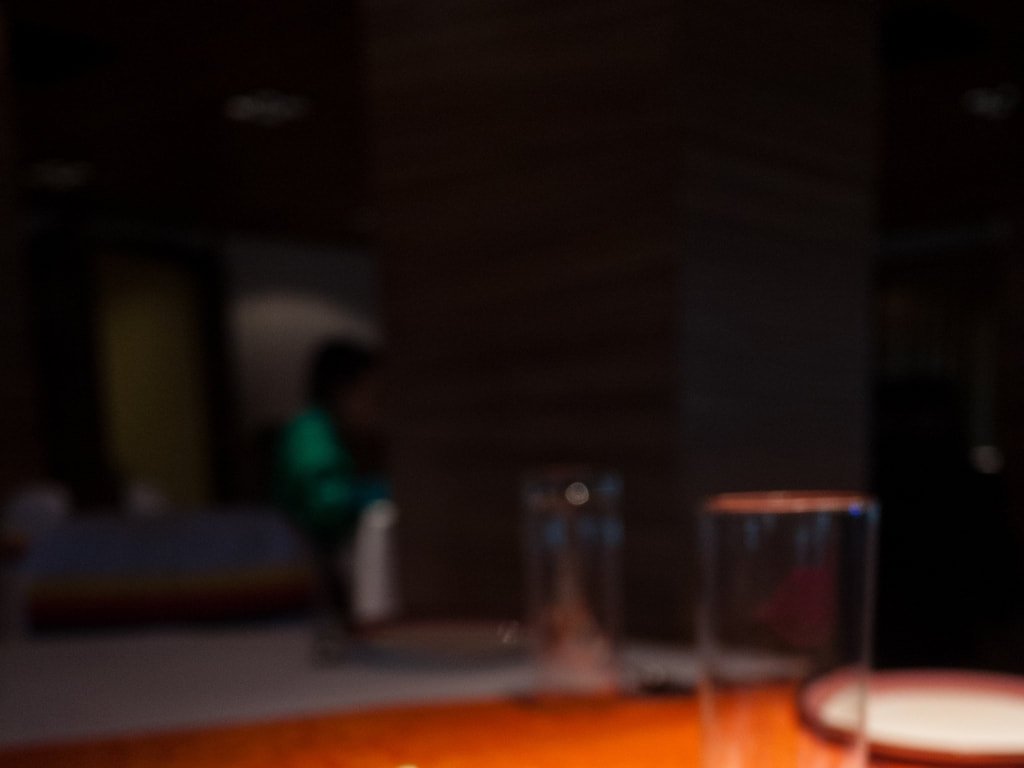
\includegraphics[height=4cm]{images/koniq-blurred.jpg}
        \caption{}
    \end{subfigure}%
    ~ 
    \begin{subfigure}[t]{0.45\textwidth}
        \centering
        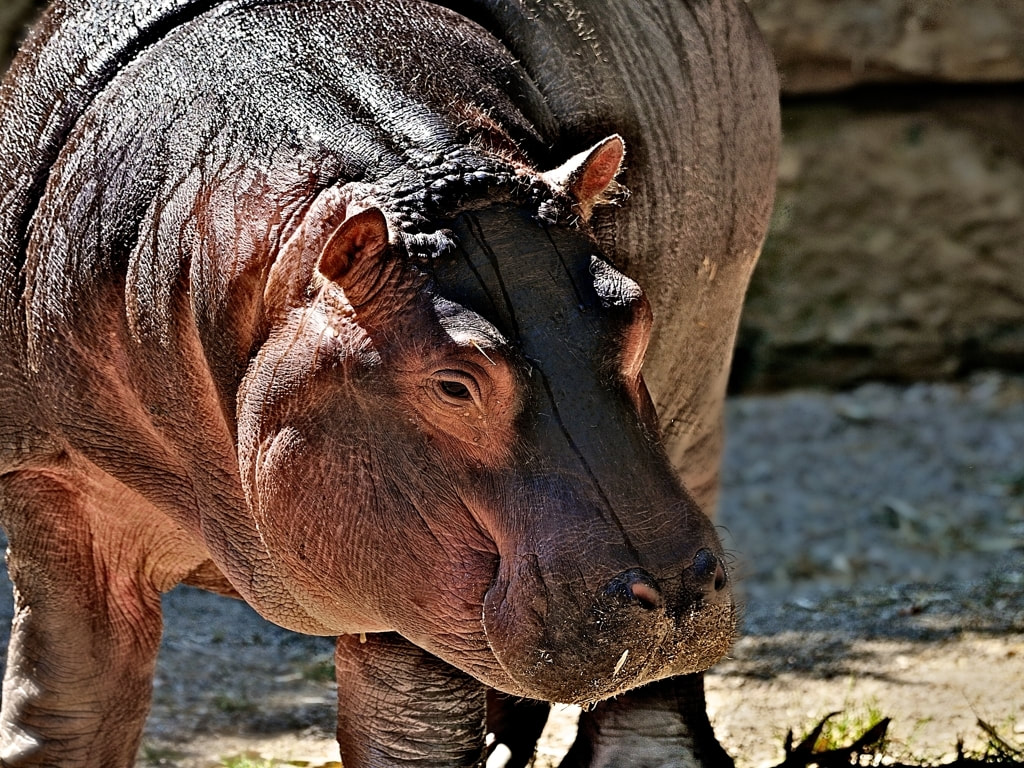
\includegraphics[height=4cm]{images/koniq-sharp.jpg}
        \caption{}
    \end{subfigure}
    \centering
    \fdireta{hosu2020koniq}
\end{figure}

\section{NR-IQA in Bright-field Microscopy Images Using the Fourier Transform and Kurtosis}
The next step is to devise a quantitative representation of sharpness for each image in each dataset. This measure allows for the selection of the eligible images through statistical analysis and the posterior registration of the selected slices. We propose a new method for image quality assessment based on a sampling process of the Fourier spectrum and posterior analysis of the coefficients as a probability distribution using summary and descriptive statistics. This section presents each stage of the method: pre-processing, Fourier spectrum sampling and statistical analysis. Figure \ref{fig:pipeline} shows a diagram of the proposed method.

\begin{figure}[ht]
  \centering
  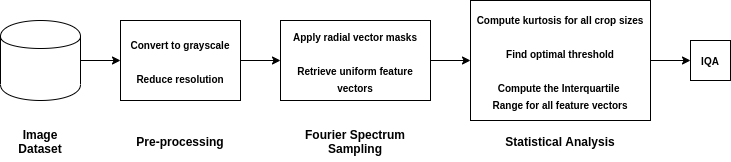
\includegraphics[scale=0.6]{images/nr-iqa_pipeline.png}
  \caption{Pipeline of processing steps of the propose no-reference IQA method.}
  \label{fig:pipeline}
\end{figure}

First, the image undergoes a grayscale conversion with the luminance method \cite{ponti2016image} - a 
linear combination of the three channels of a RGB image, as shown in the matrix equation given by

\begin{equation}
    \label{eqn:luminance}
    I_{luminance} = 0.299R + 0.587G + 0.114B,
\end{equation}

\noindent where $I_{luminance}$ is the matrix that represents the grayscale converted image, $R$, $G$ and $B$ represent the matrices of the red, green and blue channels, respectively. Next, the resolution of each grayscale image is reduced by half, from 2560 $\times$ 1920 to 1280 $\times$ 960. This provides shorter computational times. We empirically observed that  reduction in resolution did not compromise the results. We employed a bilinear interpolation that uses the four nearest neighbors to estimate the intensity at a given location \cite{gonzalez2018digital}, described as

\begin{equation}
\label{eqn:bilinear_interpolation}
I_{resized}(x,y) = ax + by + cxy + d.
\end{equation}

The CLAHE algorithm is then applied  to deliver a more uniform image to the Fourier Transform. This is necessary as microscopy images are influenced by illumination conditions, the focus adjustment itself and also physical properties of the transmitted or reflected light.

Next, the DFT is applied to all images and the resulting spectra are analyzed. The Fourier spectrum of a two-dimensional signal such as an image is a matrix with complex coefficients and zeros on each of its four corners and carries information about frequency bands of the image, characterized as a distribution. Our approach requires a shift between the first and third quadrants, and also the second and the fourth quadrants, to the center of the matrix. The unshifted and shifted Fourier spectrum of an grayscale airplane test image are shown in Figures \ref{fig:fourier_spectrum}.(c) and \ref{fig:fourier_spectrum}.(d), respectively. 

\begin{figure}[ht]
	\centering
	\caption{Original image \textbf{(a)}, luminance grayscale converted image \textbf{(b)}, unshifted Fourier spectrum of the grayscale image \textbf{(c)}, shifted Fourier spectrum of the grayscale image \textbf{(d)} and frequency bands as rings of radius $\{r_{i}: i\in\mathbb{N}^{*}\}$ drawn over the 2D spectrum \textbf{(e)}.}
	\label{fig:fourier_spectrum}
	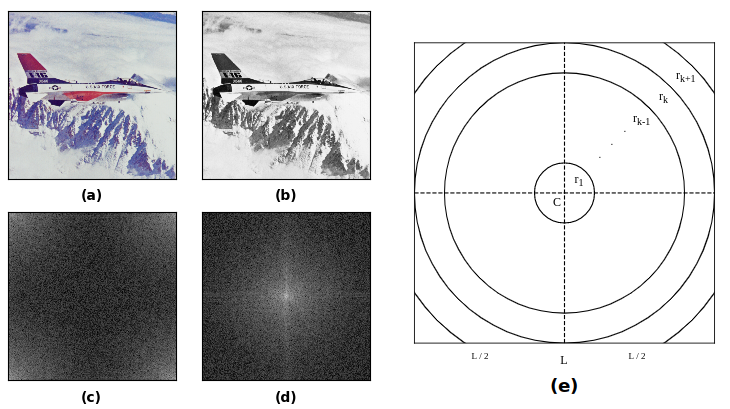
\includegraphics[scale=0.6]{images/fourier_spectrum.png}
	\centering
	\fautor
\end{figure}

The frequency information may be retrieved from the shifted Fourier spectrum by means of concentric circles drawn over it in the form of masks. Theoretically, the number of masks that may be applied to the spectra is infinite, but the discrete nature of images renders a finite number of masks. Let the matrix of DFT coefficients be graphically represented in Figure~\ref{fig:fourier_spectrum}.(e) and be mathematically denoted as a square of side $L = \max{(m,n)}$, $k = L / 2$ be the maximum radius value for circles within the square and $C = (k,k)$ be the center of the infinite set of concentric circles inscribed in the square. Circles with small radii comprise low-frequency information whereas large radii values cover high-frequency coefficients.

Taking into account the pixel resolution of the input images, it makes sense to sample the information, otherwise, the computational complexity and running times of the algorithm for one image alone would be impractical. Moreover, it is also unrealistic to evaluate every area under each concentric circle to retrieve the frequency content of an image; there is also no standard discrete amount of frequency bands to be evaluated.

Therefore, we drove our efforts to comprise as much information about each frequency band as possible and explored the fact that the Fourier spectrum of a real function such as an image is even, i.e. symmetric concerning its origin. Instead of the pure complex coefficients, we represent the Fourier spectrum by the magnitude of its coefficients, given by

\begin{equation}
\label{eqn:magnitude_of_DFT}
K(m,n) = 
    \log_{e}{\left(1
    + \sqrt{
        [\operatorname{Re}{(\hat{g}(m,n))}]^{2}
        + [\operatorname{Im}{(\hat{g}(m,n))}]^{2}
      }
    \right)},
\end{equation}

\noindent where $\hat{g}(m,n)$ are the complex Fourier coefficients of an image $g(x,y)$. We propose to sample the spectrum by means of radial lines as masks, i.e. white antialiased lines are drawn over a zero-valued matrix of dimensions 1280 $\times$ 960, the same dimensions of the Fourier spectrum of the reduced image, which are then element-wise multiplied by the spectrum. The lines are created from the $(x_{c},y_{c})$ center of the spectrum to points in an approximate radial position, which is calculated by

\begin{equation}
\label{eqn:points_on_radii}
P(x,y) = 
    (
    x_{c} r_{j} \cos{a_{j}}, 
    y_{c} r_{j} \sin{a_{j}}
    )
\end{equation}

\noindent with the set of angles $\{a_{j}\}$ in the radian form, computed as

\begin{align}
\label{eqn:angles}
\left\{
a_{j} : a_{j} = 
\frac{j \pi}{180}
\right\}
&&  j = \{0,5,...,100\}.
\end{align}

Equation
\ref{eqn:points_on_radii} is a
floating-point ordered pair, rounded to the nearest integer value in order to represent a location in the spectrum. The
antialiased lines are drawn with a Gaussian filtering process. After all the lines have been generated, the mask is similar to what is shown in Figure~\ref{fig:radial_masks}:

\begin{figure}[ht]
	\centering
	\caption{Final mask of antialised radial lines to sample the Fourier spectrum.}
	\label{fig:radial_masks}
	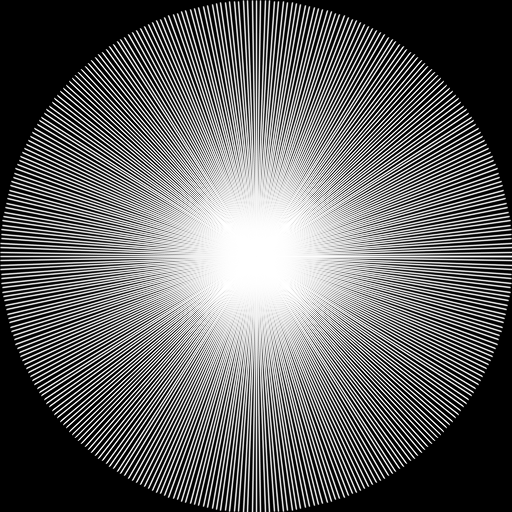
\includegraphics[scale=0.5]{images/radial_masks.png}
	\centering
	\fautor
\end{figure}

The extraction of the region of interest from the spectrum with the mask of radial lines results in arrays of complex coefficients that represent samples of the frequency profile of the image. However, despite the antialiasing, the resulting arrays differ in length since the original data is discrete. The vectors go through an element-wise average, which results in a one-dimensional vector as a descriptor of the frequency spectrum, and before such average, we find the smallest vector size among all of them and discard the remaining information in all of them. For comparison purposes, a square image of side $L$ yields a feature vector of size $1 / 2L$.

Next, the sharpness information of the image is encoded into a low-dimensional and concise representation that may undergo analysis with statistical tools and the mathematical properties of the Fourier spectrum. The feature vectors from each image need to be transformed into a model that is suitable for techniques such as Descriptive Statistics or Bayesian Inference, and therefore must be mapped onto the probability space $\Omega = [0,1]$. Hence, we apply an operator $T : \ell^{2}(\mathbb{Z}^{2}) \rightarrow \ell^{2}(\mathbb{Z}^{2})$, written as

\begin{align}
\label{eqn:probability_operator}
T(x_{i}) = \frac{x_{i}}{\sum_{j=0}^{n-1}x_{j}}
&&  i = \{0,1,...,n-1\},
\end{align}

\noindent where each $x_{i}$ is a value of the descriptor which will be mapped onto a probability. Note that each feature vector after the sampling process is a distribution in the scope of the Distribution Theory, i.e. a continuous linear functional defined on a space of smooth (functions with continuous derivatives up to some desired order over some domain \cite{weisstein2020smooth}) and compact supported (the functions yields zero outside of a closed and bounded set \cite{weisstein2020compact}) functions, with values in the range $[0,\infty)$. Therefore, it makes sense to apply the operator that maps it to a probability. This proposition was proved in \autoref{chapter:definitions-and-proofs}, which summarizes several definitions from Mathematical Analysis, Measure Theory and Distribution Theory required for the proof.

Information embedded in the low-frequency components of each feature vector corresponds to the Dirac delta distribution within the PSF of the microscope and should be discarded since it is equal to all images and does not resemble blur information; the removal should be done with caution so that the remaining information is enough to represent the blur profile of the image and allow the further selection by the image quality metric. An optimal threshold should be calculated for ``cropping'' the data, i.e. only a subset of it will represent the sharpness information. The threshold is chosen to maximize the difference between the maximum and the minimum among a set of kurtosis values of each feature vector.

The array of kurtosis for every crop size is computed as follows. The crop size initializes as zero and is used to compute the kurtosis of the entire set $\{x_{1},x_{2},...,x_{n}\}$ of all descriptors. The crop size is then incremented by 1, yielding the subset $\{x_{2},x_{3},...,x_{n}\}$. This process is done until the kurtosis for all crop sizes of the feature vectors is computed. Algorithm \ref{alg:kurtosis_array} summarizes the computation of kurtosis for all crop sizes:

\begin{algorithm}[H]
	\caption{Kurtosis computation}
	\label{alg:kurtosis_array}
	\begin{algorithmic}[1]
	    \State // $X_{c \times n}$: dataset of $n$ descriptors with size $c \in C$, where \\ // $C = \{0,1,...,size(descriptor)\}$ 
	    
	    \\
	    
	    \State // $T(X)$: operator from equation \ref{eqn:probability_operator} to map the \\ // descriptors onto probability distributions
	   
        \\
        
		\State $X \gets T(X)$
		\State $A \gets zeros(c, n)$
		
		\For {\textbf{each} crop size $c$ in $C$}
		    \For{\textbf{each} descriptor $i$ in $\{1,2,...,n\}$}
		
        		\State $A[crop][i] \gets$ \textbf{kurtosis}$\left(X[i].subset(0, crop)\right)$
		
		    \EndFor
		\EndFor
		
		\\
		
		\Return $A$
	\end{algorithmic}
\end{algorithm}

\noindent Next, the optimal threshold computation is done with algorithm~\ref{alg:cut_threshold}. It aims to produce a crop size to maximize the peak to peak value, i.e. the difference between the maximum and minimum values in the dataset. This allows low-frequency information to be discarded from the PSF without loss of the blur.

\begin{algorithm}[ht]
	\caption{Find the optimal dataset variability threshold}
	\label{alg:cut_threshold}
	\begin{algorithmic}[1]
 		\State // $A_{c \times n}$: matrix with kurtosis values for all $n$ descriptors that were computed at every crop \\ // size $c \in C$, where \\ // $C = \{0,1,...,size(descriptor)\}$ 
		
		\\
		
		\State $threshold \gets 0$
		\State $maximum \gets \infty$
		\For {\textbf{each} crop size $c$ in $C$}
		\State $row \gets \{A_{c,1},A_{c,2},...,A_{c,n}\}$ 
		
		\State $a \gets$ \textbf{max}$(row)$
		
		\State $b \gets$ \textbf{min}$(row)$
		
		\\
		
		\If{$a < 0$ or $b < 0$}
		    \State \textbf{continue}
		\EndIf
		
		\\
		
		\State $range \gets a - b$
		
		\\
		
		\If{$range > maximum$}
		    \State $maximum \gets range$
		    \State $threshold \gets c$
		\EndIf
		
		\EndFor
		\\
		\Return $threshold$
% 		\EndFunction
	\end{algorithmic}
\end{algorithm}

The low-frequency is discarded in each feature vector up to the optimal threshold, and the IQR measure is computed for all of them. In this work, the IQR value of the feature vector of an image corresponds to the amount of details, i.e. high-frequency content on it: the higher the IQR value, the sharper the image is. Finally, an estimate of the subset of images that is eligible for the fusion process is then obtained by the $z$-score transformation by choosing the images that locate at one or more standard deviation units away from the mean.

\section{Laplacian of Gaussian-based Multi-focus Bright-field Microscopy Image Fusion}
The NR-IQA method provided a sharpness measure for each image of the datasets and such numerical representations were analyzed with the $z$-score; at this point, the estimate of eligible images was prompted to the user and the real eligible ones were chosen. The obtained subset is registered by means of the SIFT-based z-stack alignment tool of the TrakEM2 package. The subsequent stage is to perform the fusion of images in the before-mentioned subset. We propose a multi-focus bright-field microscopy image fusion algorithm with the Laplacian of Gaussian edge detection filter and the energy of edges. Fig.~\ref{fig:fusion_pipeline} shows a diagram of the proposed method.

\begin{figure}[ht]
    \centering
    \caption{Diagram of the proposed multi-focus bright-field microscopy image fusion algorithm.}
    \label{fig:fusion_pipeline}
    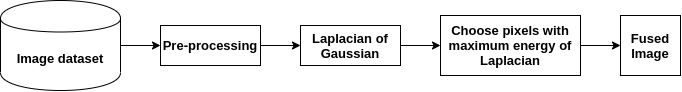
\includegraphics[scale=0.65]{images/fusion_pipeline.png}
    \centering
    \fautor
\end{figure}

The grayscale version of the selected images is again used for fusion; since the images were converted with the luminance method, the edges are preserved and therefore the edge detection may be successful. Other methods from the \emph{Luminance} family, e.g. \emph{Luminance}, \emph{Luminance\'}, \emph{Luma} and \emph{Decolorize}, are also suitable \cite{kanan2012color}.

The images then undergo the Laplacian of Gaussian filter - a spatial filtering algorithm that extracts edges of a smoothed image. The Laplacian is a second-order derivative isotropic linear operator, based on the Laplacian of a function, which defines an edge as the zero-crossing of the second derivative of a function. First and foremost, the Laplacian of a function is denoted by

\begin{equation}
\label{eqn:laplacian_of_function}
\nabla^{2}g(x,y) = \frac{\partial^{2} g(x,y)}{\partial x^{2}}
                    +
                  \frac{\partial^{2} g(x,y)}{\partial y^{2}},
\end{equation}

\noindent where $g(x,y)$ is the input image. For the discrete case (which applies to the digital images), the Laplacian operator is achieved by means of a convolution. The approximation of the second derivatives in each dimension yields the following convolution kernel

\begin{equation*}
\label{eqn:discrete_laplacian}
\begin{bmatrix}
0 & 1 & 0 \\
1 & -4 & 1 \\
0 & 1 & 0
\end{bmatrix}.
\end{equation*}

Similarly, instead of extracting edges with the Laplacian filter only, the Laplacian of Gaussian filter performs a Gaussian filtering process to remove noise and smooth the images before retrieving the edges \cite{marr1980theory}. This approach applies to cases where the quality and reliability of edges obtained by the Laplacian operator are sensitive to noise, and also plays the role of distinguishing the blurry regions from the sharp ones in our approach; pixels belonging to sharp regions will suffer a stronger smoothing effect in comparison to blurry pixels. For our application, an image is convolved with a two-dimensional Gaussian filter, denoted by

\begin{equation}
\label{eqn:gaussian_filter}
S(x,y) = g(x,y) \ast \frac{1}{\sqrt{2 \pi \sigma}} e^{- \frac{x^{2} + y^{2}}{\sigma^{2}}},
\end{equation}

\noindent where $S(x,y)$ is the smoothed version of the image, $g(x,y)$ is the input image and $\sigma$ is the standard deviation of the Gaussian function. Then, the Laplacian is applied to the smoothed image $S$. Both operators are linear and shift-invariant and therefore can be applied in any order, but the Gaussian filter is commonly applied first if the application required separated filters. In our case, the Laplacian of Gaussian operator can be defined as

\begin{equation}
\label{eqn:laplacian_of_gaussian}
LoG(x,y) = - \frac{1}{\pi \sigma^{4}}
            \left[
                1 - \frac{(x^{2} + y^{2})}{2 \sigma^{2}}
            \right]
            e^{- \frac{x^{2} + y^{2}}{2 \sigma^{2}}}.
\end{equation}

\noindent The $\sigma$ parameter is responsible for the smoothing magnitude. The convolution kernel is then a combination of both Laplacian and Gaussian filters; higher $\sigma$ values increase the effective kernel size consequently the smoothing effect. The next step is to retrieve the energy for each region, also based on the fact that blurry regions of an image present less high-frequency components than sharp regions. This stems from the fact that sharp regions are prone to have more edges than smoothed ones, hence a higher energy level. The higher the number the edges in an area of the image, the better the focus on it. Therefore, pixels that correspond to edges are chosen to form the fused image. Their spatial location is used to construct an RGB image by retrieving the content of the three channels from those pixels and assigning them to the final image.

\chapter{Results}
\label{chapter:results}
Experiments have been carried out for the two proposed methods: a) the NR-IQA  and b) multi-focus image fusion, both with bright-field microscopy. In this chapter, we report the performance of our methods on the created datasets and described in \autoref{chapter:materials-and-methods}. We also present the quantitative evaluation metrics used. Both IQA and image fusion experiments have been conducted on an Intel Core i7 CPU computer with 8 GB RAM, running Ubuntu Linux 18.04 64-bit.

Concerning the IQA method, the proposed labels, i.e. ``eligible'' and ``negligible'', are a subjective quality score. According to \citeonline{wang2011information}, evaluation metrics such as the Pearson Linear Correlation Coefficient (PLCC), the Spearman's Rank Correlation Coefficient (SRCC) and the Kendall's Rank Correlation Coefficient (KRCC) are quantitive methods that relate to our comparison and are suitable for the case. For all correlation coefficients, higher values yield higher reliability to the objective IQA metric.

According to \citeonline{chen2002correlation}, the PLCC (also named Pearson's r coefficient) is the most widely used correlation coefficient. It characterizes the degree of the association between linearly related variables and is given by

\begin{equation}
\label{eqn:plcc}
r_{xy} = \frac{n \sum x_{i} y_{i} - \sum x_{i} \sum y_{i}}{\sqrt{n \sum x_{i}^{2} \left(\sum x_{i}\right)^{2} n \sum y_{i}^{2} \left(\sum y_{i}\right)^{2}}},
\end{equation}

\noindent where $r_{xy}$ is the r correlation coefficient between the $x$ and $y$ variables, $n$ is the number of observations of both variables, $x_{i}$ is the value of $x$ for the $i$th observation and $y_{i}$ is the value of $y$ for the $i$th observation. Still, according to \citeonline{chen2002correlation}, the KRCC and SRCC are non-parametric tests that also measure the strength of dependence between two variables. They may be denoted as

\begin{equation}
\label{eqn:krcc}
\tau = \frac{n_{c} - n_{d}}{\frac{1}{2} n \left(n-1 \right)}
\end{equation}

\begin{equation}
\label{eqn:srcc}
\rho = 1 - \frac{6 \sum d_{i}^{2}}{n \left(n^{2}-1 \right)},
\end{equation}

\noindent where $\tau$ and $\rho$ denote the KRCC and SRCC measures, respectively. For both equations, $n$ is the number of observations of both variables. In \autoref{eqn:krcc}, $n_{c}$ and $n_{d}$ are the number of concordant and discordant observations, i.e. ordered in the same and in different ways, respectively. In addition, $d_{i}$ in \autoref{eqn:srcc} denotes the difference between the ranks of corresponding variables.

Similarly, we propose the use of Entropy, Spatial Frequency (SF) and the Standard Deviation (STD) for the evaluation of our image fusion method \cite{naidu2008pixel}. The Entropy measures the information content of an image and is denoted as

\begin{equation}
\label{eqn:entropy}
He = - \sum_{i = 0}^{L} h(i) \log_2 h(i),
\end{equation}

\noindent where $h(i)$ is the normalized histogram of the fused image and $L$ is the number of bins of such histogram. The higher the Entropy value, the more details the fused image has, i.e. the sharper it is. The Spatial Frequency presents the overall activity level in the fused image by means of the amount of information in the rows and columns, given by

\begin{equation*}
RF = \sqrt{\frac{1}{M N} 
            \sum_{x = 1}^{M}
            \sum_{y = 2}^{N}
            \left[
                I(x,y) - I(x,y - 1)
            \right]^{2}
}
\end{equation*}

\vspace{0.25cm}

\begin{equation*}
CF = \sqrt{\frac{1}{M N} 
            \sum_{y = 1}^{N}
            \sum_{x = 2}^{M}
            \left[
                I(x,y) - I(x - 1,y)
            \right]^{2}
}
\end{equation*}

\vspace{0.25cm}

\begin{equation}
\label{eqn:spatial_frequency}
SF = \sqrt{RF^{2} + CF^{2}},
\end{equation}

\noindent where $I(x,y)$ is the fused image and $M$, $N$ are the image width and height, respectively. Higher values indicate better fusion quality since more activity means less homogeneous regions in our case. Finally, the Standard Deviation measures the contrast in the fused image, and therefore higher values yield higher contrast. It may be obtained as

\begin{align}
\label{eqn:standard_deviation}
STD = \sqrt{\sum_{i = 0}^{L}}(i - \Bar{i})^{2} h(i),
&&
\Bar{i} = \sum_{i = 0}^{L}i h(i).
\end{align}

\noindent with $h(i)$ and $L$ as defined in \autoref{eqn:entropy}.

\section{Image Quality Assessment}
The NR-IQA method was developed first, and our results with well-known NR-IQA approaches such as MLV \cite{bahrami2014fast}, $S_{3}$ \cite{vu2012s3}, JNB \cite{ferzli2009noreference}, CPBD \cite{narvekar2011noreference}, Marziliano \textit{et. al.} \cite{marziliano2002noreference} and Kanjar \cite{kanjar2013image}. \autoref{tab:iqa_performance_comparison} shows the results of the PLCC, SRCC and KRCC metrics for the \textit{Callisia}, \textit{Tradescantia} and \textit{Cthenante} datasets, respectively.

\begin{table}[ht]
    \centering
    \caption{Performance comparison of our proposed method and other NR-IQA metrics on the microscopy images datasets.}
    \label{tab:iqa_performance_comparison}
    \begin{tabular}{lcccccccc}
        \toprule
        Dataset & Index & MLV & $S_{3}$ & JNB & CPBD & Marz. & Kanjar & \textbf{Proposed}\\
        \midrule
        
        \multirow{3}{*}{\textit{\small Callisia}} 
        & \small PLCC & 0.2829 & 0.1752 & 0.5461 & 0.7361 & 0.7457 & 0.6688 & \textbf{0.7488}\\
        & \small SRCC & 0.2752 & 0.1730 & 0.6031 & 0.6122 & 0.6122 & 0.5971 & \textbf{0.6212}\\
        & \small KRCC & 0.2267 & 0.1425 & 0.4968 & 0.5043 & 0.5043 & 0.4919 & \textbf{0.5117}\\
        
        \midrule
        
        \multirow{3}{*}{\textit{\small Tradescantia}}
        & \small PLCC & 0.1285 & -0.1312 & 0.2561 & 0.2409 & 0.2322 & 0.2564 & \textbf{0.3698}\\
        & \small SRCC & 0.1346 & -0.1253 & 0.2181 & 0.2413 & 0.2227 & 0.2227 & \textbf{0.2552}\\
        & \small KRCC & 0.1107 & -0.1031 & 0.1794 & 0.1985 & 0.1832 & 0.1833 & \textbf{0.2099}\\

        \midrule
        
        \multirow{3}{*}{\textit{\small Cthenante}} 
        & \small PLCC & 0.0446 & -0.1682 & 0.7840 & 0.8041 & 0.8012 & 0.7831 & \textbf{0.8129}\\
        & \small SRCC & 0.0227 & -0.2068 & 0.7414 & \textbf{0.7515} & 0.7464 & 0.7338 & 0.7414\\
        & \small KRCC & 0.0187 & -0.1704 & 0.6108 & \textbf{0.6191} & 0.6150 & 0.6046 & 0.6108\\
        
        \bottomrule
    \end{tabular}
    \centering
    \fautor
\end{table}


From \autoref{tab:iqa_performance_comparison}, we may conclude that our tests obtained reasonable results with the proposed microscopy images. Our method obtained the highest values for most of the metrics in most of the datasets.  The difference between our images and benchmark datasets such as LIVE \cite{sheikh2006statistical} and CSIQ \cite{larson2010most} is that our bright-field microscopy images are subjected to a non-homogeneous blur kernel and the spherical aberrations are more prominent. Consequently, the labeling of blurred and sharp is subjective, since the notion of quality might be different according to what the images will be used for. In the scope of this work, the reason for assessing image quality is to predict eligible images and select the proper ones to perform the fusion process.

The PLCC, SRCC and KRCC coefficients also evaluate the \textit{monotonicity}, i.e. the property of maintaining the order relation between the sets - it is only nondecreasing or nonincreasing. In this work, monotonicity relates the values obtained by applying our metric on the proposed datasets and the set of labels provided by the subject evaluation of them. The results in \autoref{tab:iqa_performance_comparison} also show how monotonic the metric is. Finally, the computational performance of an NR-IQA metric may be a constraint. Autofocus systems in microscopes, for example, should be capable of updating sharpness metrics several times to find the best focus setup. Our method was built with the C++ language and the OpenCV framework in order to achieve good computational performance with common hardware and operating system settings and is available in a repository. We also implemented the Kanjar method in Python, and the code is also organized in a repository. 

The literature NR-IQA methods we used to compare our results were implemented in MATLAB, C++ and Python programming languages. The implementations we used are summarized in \autoref{tab:implementations}:

\begin{table}[htbp]
    \caption{Implementations of the literature IQA methods and ours.}
    \label{tab:implementations}
    \begin{center}
    \begin{tabular}{lcc}
        \toprule
        \textbf{Method} & \textbf{Environment} & \textbf{Implementation}\\
        \midrule
        MLV & MATLAB & \url{https://sites.google.com/site/khosrobahrami2010/publications}\\
        $S_{3}$ & MATLAB & \url{http://vision.eng.shizuoka.ac.jp/s3/}\\
        JNB & MATLAB & \url{https://ivulab.asu.edu/software/jnbm/}\\
        CPBD & Python & \url{https://pypi.org/project/cpbd/}\\
        Marz. & C++ & \url{https://github.com/PeterWang1986/blur}\\
        Kanjar & Python & \url{https://github.com/vaugusto92/kanjar-nr-iqa}\\
        Proposed & C++ & \url{https://github.com/vaugusto92/fourier-light-microscopy-nr-ism}\\
        \bottomrule
    \end{tabular}
\end{center}
\end{table}


\autoref{tab:running_times_comparison} presents the running time comparison for all methods in the three proposed datasets. Despite the programming language differences, our method yielded a relevant computational efficiency in terms of execution time. 

\begin{table}[ht]
    \centering
    \caption{Running times for the proposed method and other NR-IQA metrics on our \emph{Callisia repens} microscopy images dataset.}
    \label{tab:running_times_comparison}
    \begin{tabular}{lccccccc}
        \toprule
        & \multicolumn{7}{c}{Times} \\
        \midrule
        Dataset & MLV & $S_{3}$ & JNB & CPBD & Marz. & Kanjar & \textbf{Proposed}\\
        \midrule
        
        \textit{Callisia} & 00:01:06 & 04:25:00 & 00:04:37 & 00:14:00 & \textbf{00:00:08} & 00:00:25 & 00:00:13\\
        \textit{Tradescantia} & 00:01:55 & 00:49:30 & 00:05:42 & 00:14:31 & \textbf{00:00:09} & 00:00:30 & 00:00:20\\
        \textit{Cthenante} & 00:01:31 & 03:17:16 & 00:04:28 & 00:14:47 & \textbf{00:00:06} & 00:00:24 & 00:00:11\\
        
        \bottomrule
    \end{tabular}
    \centering
    \fautor
\end{table}

\section{Image Fusion}
The proposed method was implemented in Python programming language with the NumPy, Scipy, scikit-image and Pillow libraries. Following reproducible research ideals, the code is organized and made available in a repository \footnote{\url{https://github.com/vaugusto92/light-microscopy-image-fusion-prototype}}.

We compared our proposed method with well-known multi-focus image fusion approaches such as PCA \cite{naidu2008pixel}, GF \cite{li2013image}, MSWG \cite{zhou2014multi}, and MSVD \cite{naidu2011image}. The optimal value for the $\sigma$ parameter was empirically acquired, and was set to $0.7$. \autoref{tab:fusion_performance_comparison} shows the results of the Entropy, MSSIM and STD metrics for the \textit{Callisia}, \textit{Tradescantia} and \textit{Cthenante} datasets with each fusion approach.

\begin{table}[ht]
    \centering
    \caption{Objective performance evaluation of the proposed method ($\sigma = 0.7$) and other image fusion approaches.}
    \label{tab:fusion_performance_comparison}
    \begin{tabular}{lcccccc}
        \toprule
        Dataset & Index & PCA & GF & MSWG & MSVD & \textbf{Proposed}\\
        \midrule
        
        \multirow{3}{*}{\textit{\small Callisia}} 
        & \small Entropy & 10.9928 & 11.3332 & 11.7052 & 11.4759 & \textbf{12.1904}\\
        & \small SF & 0.0253 & 0.0347 & 0.0441 & 0.0424 & \textbf{0.0836}\\
        & \small STD & 0.1966 & 0.1939 & 0.1949 & 0.1968 & \textbf{0.1987}\\
        
        \midrule
        
        \multirow{3}{*}{\textit{\small Tradescantia}}
        & \small Entropy & 8.4619 & 9.2162 & 9.2120 & 8.6751 & \textbf{9.3011}\\
        & \small SF & 0.0167 & 0.0249 & 0.0250 & 0.0219 & \textbf{0.0286}\\
        & \small STD & 0.0809 & \textbf{0.0826} & 0.0825 & 0.0811 & 0.0816\\
        
        \midrule

        \multirow{3}{*}{\textit{\small Cthenante}}
        & \small Entropy & 6.7263 & 6.7577 & 3.6411 & \textbf{7.7962} & 4.3565\\
        & \small SF & 0.0317 & 0.0473 & 0.0645 & 0.0482 & \textbf{0.0881}\\
        & \small STD & 0.0810 & 0.0760 & 0.0815 & 0.0827 & \textbf{0.1117}\\

        \bottomrule
    \end{tabular}
    \centering
    \fautor
\end{table}

The values in \autoref{tab:fusion_performance_comparison} show that the proposed method yields better results when compared to the well-known multi-focus image fusion methods in the bright-field microscopy z-stacks. Our image dataset differs from benchmarks such as the Lytro \cite{nejati2015multi}. As seen in \autoref{chapter:blur-characterization-and-image-formation}, the image formation is subject to anisotropic blur kernels due to the optical properties of the lenses in bright-field microscopy. In the benchmark images, it is possible to precisely point out the blurred and sharp regions, since there are usually two or three images of each scene; our dataset, on the other hand, does not allow this. Thus, the fusion results for benchmark datasets reach optimal performance, and some of them even contain the reference image for a better comparison. Finally, the fusion rule should be robust to noise and should have a large variation with respect to the degree of blurring \cite{huang2007evaluation}. The Gaussian smoothing procedure provides robustness to noise in our algorithm. 

We also present the qualitative results, i.e. the fused images and some samples of each dataset. With the results from our IQA method, we have selected the eligible slices in each dataset and registered with the TrakEM2 alignment tool. The \textit{Callisia} dataset has six slices which present slight differences between the background of the leaf and the stomata. The images in this dataset are the brightest among all images in our datasets. Two eligible slices were obtained in the \textit{Tradescantia} dataset due to its large magnification, where either background sections or stomata are focused. Also, images in this dataset are not as bright as \textit{Callisia} ones, as the specimens present a strong purple color in their abaxial region. Finally, the \textit{Cthenante} dataset presents the strongest difference in focused regions among all datasets and also the darkest images. The results of the fusion process of \textit{Callisia}, \textit{Tradescantia} and \textit{Cthennante} are shown in \autoref{fig:fused_callisia}, \autoref{fig:fused_tradescantia} and \autoref{fig:fused_cthenante}, respectively, while \autoref{fig:registered_slices} depicts samples of registered images in each dataset. 

\begin{figure}[H]
  \centering
  \caption{Fused \textit{Callisia} image.}
  \label{fig:fused_callisia}
  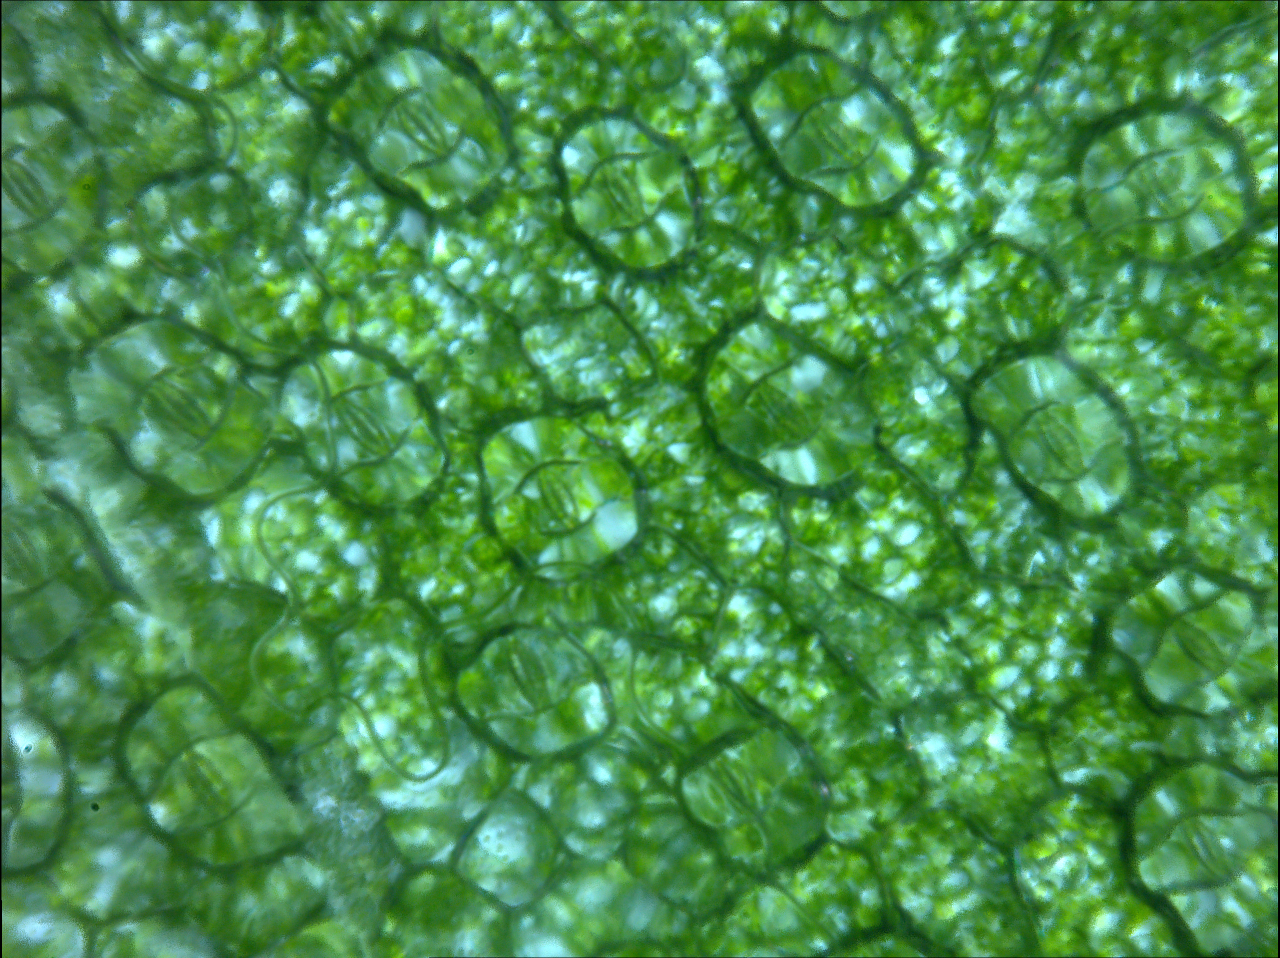
\includegraphics[scale=0.3]{images/fused_callisia.png}
  \centering
  \fautor
\end{figure}

\begin{figure}[H]
    \centering
    \caption{Fused \textit{Tradescantia} image.}
    \label{fig:fused_tradescantia}
    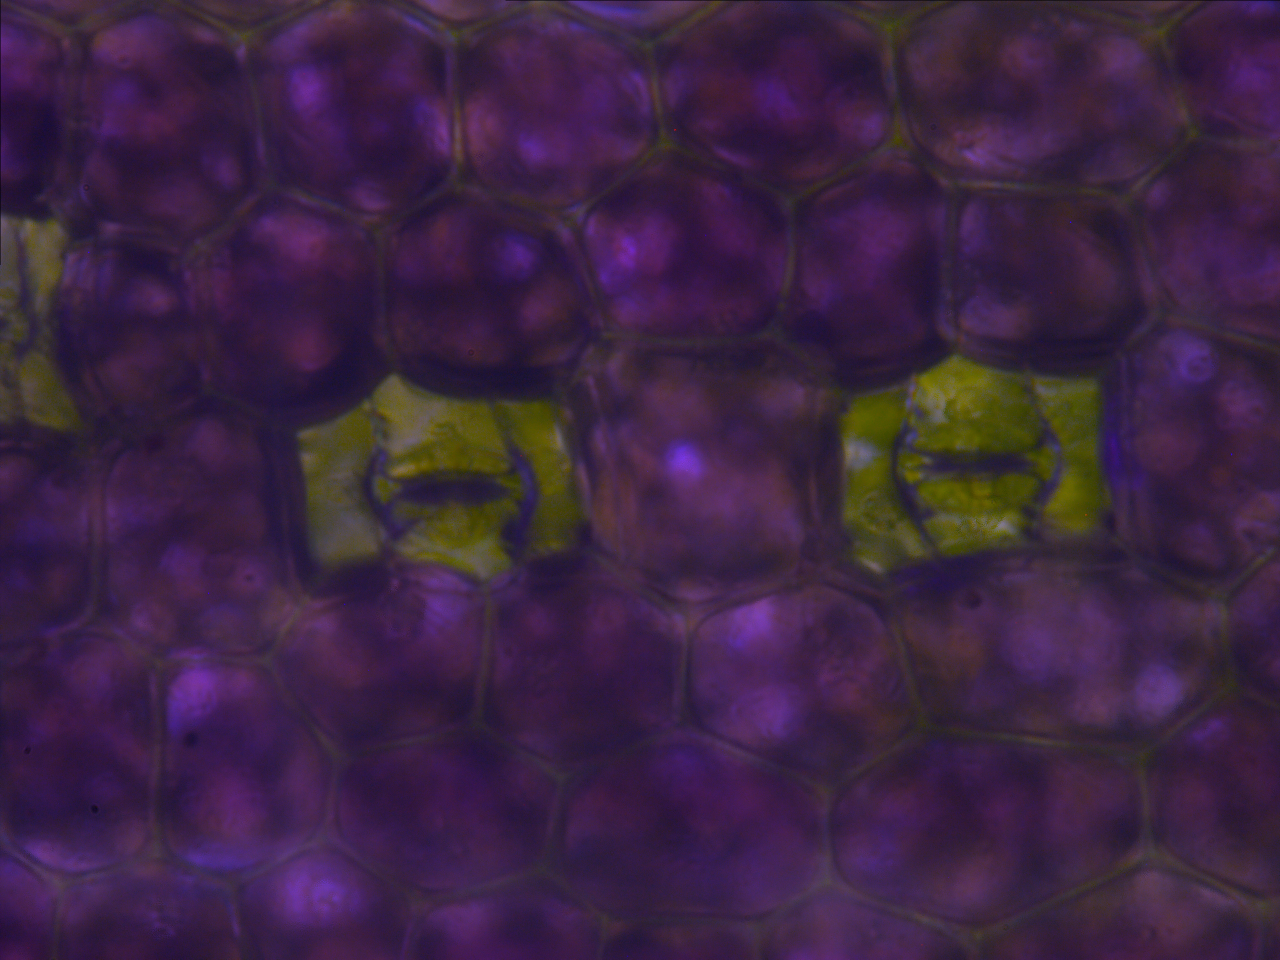
\includegraphics[scale=0.3]{images/fused_tradescantia.png}
    \centering
    \fautor
\end{figure}

\begin{figure}[H]
  \centering
  \caption{Fused \textit{Cthenante} image.}
  \label{fig:fused_cthenante}
  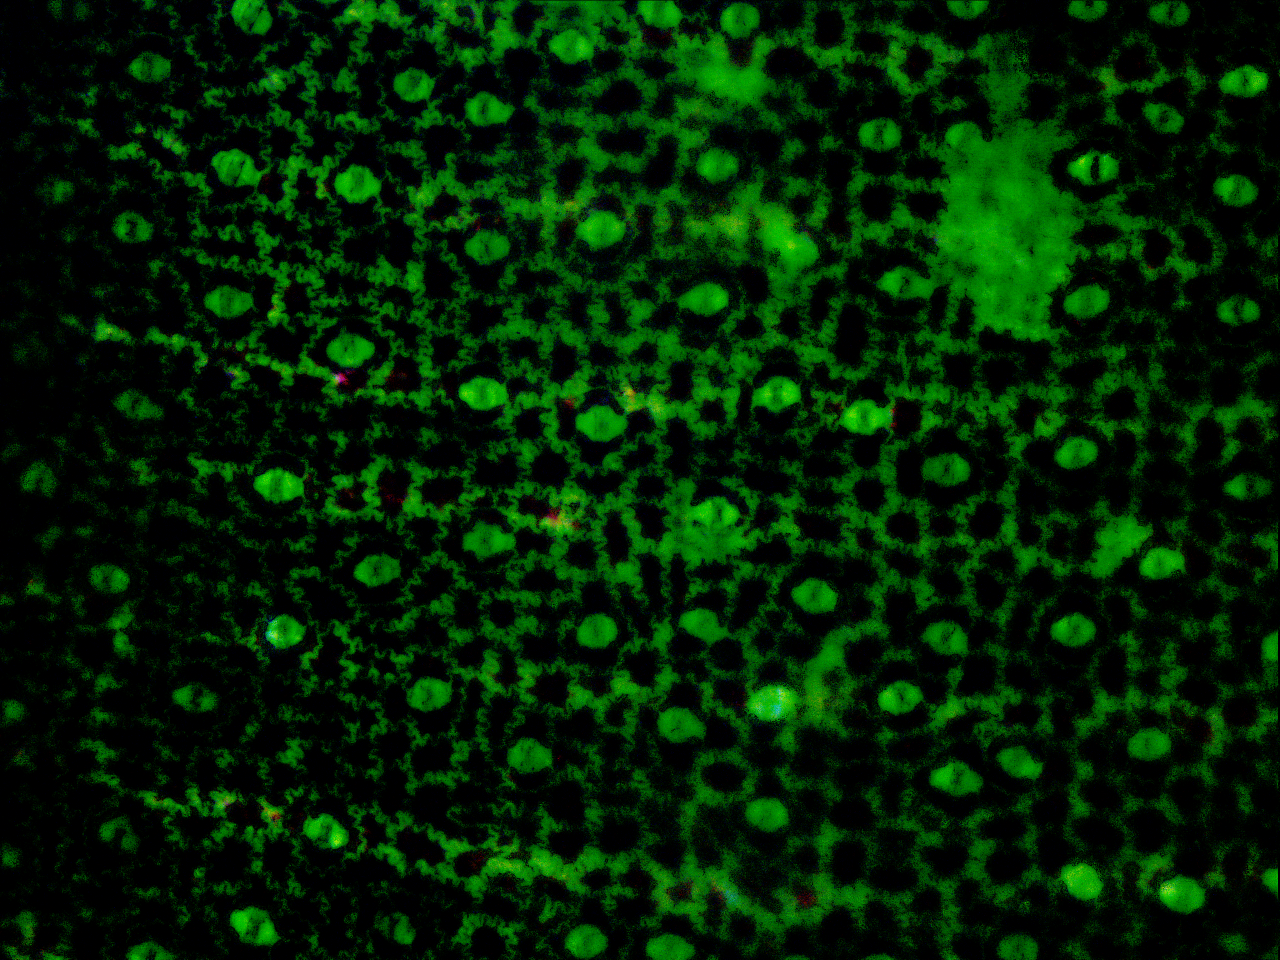
\includegraphics[scale=0.3]{images/fused_cthenante.png}
  \centering
  \fautor
\end{figure}

\begin{figure}[htb]
    \centering
    \caption{Registered slices of our \textit{Callisia} (a), \textit{Tradescantia} (b) and \textit{Cthenante} (c) datasets.}
    \label{fig:registered_slices}
    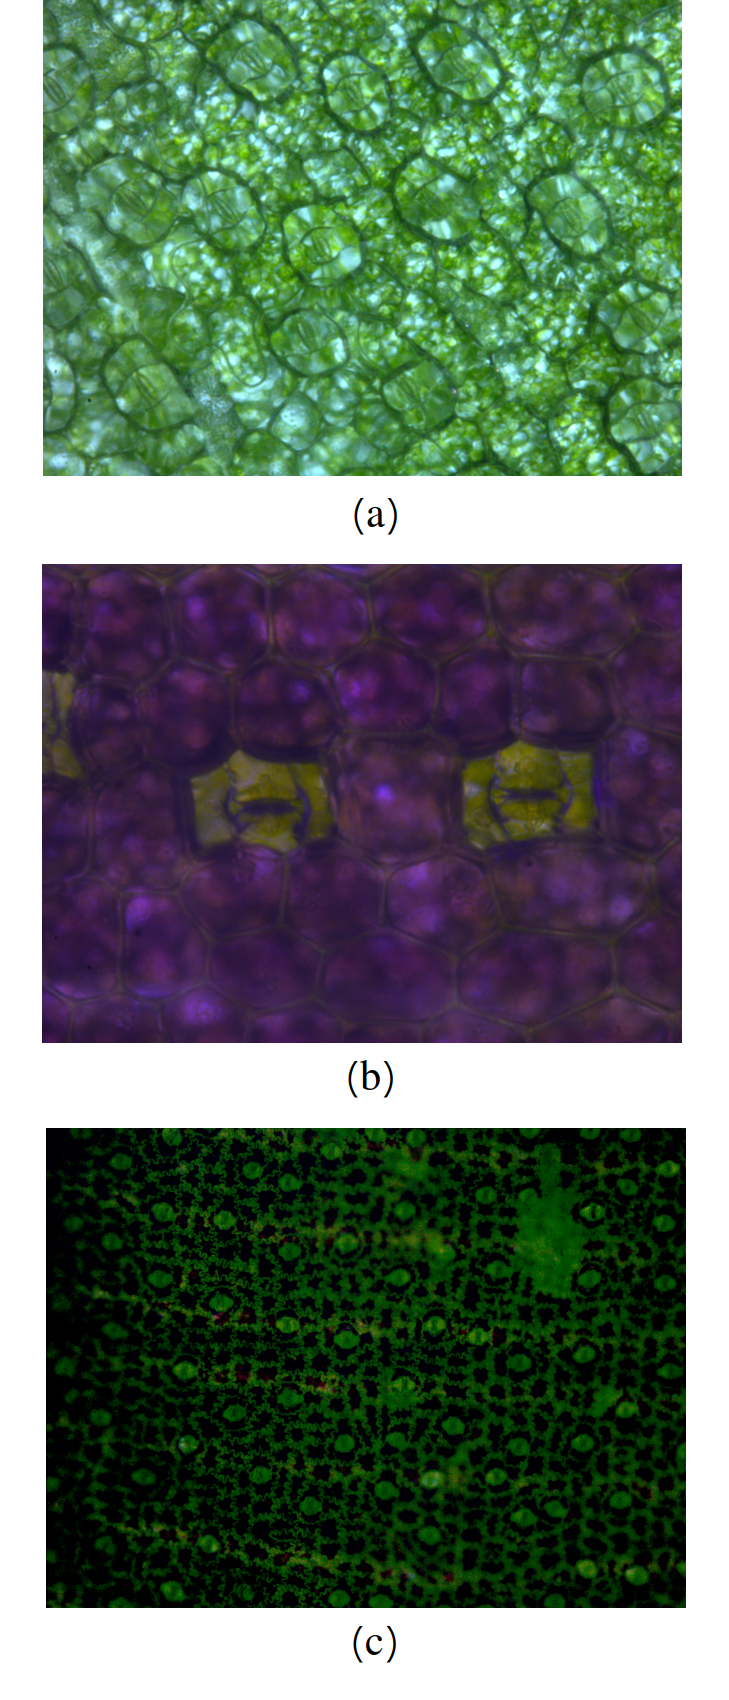
\includegraphics[scale=.32]{images/middle_images.png} \centering
    \fautor
\end{figure}

Each of the images in \autoref{fig:registered_slices} represent the middle of the z-stack. For example, \autoref{fig:registered_slices}.(c) is blurred on the left and right parts and sharp in the middle section; this shows that the leaf has a slope structure that promoted a clear division between blurred and sharp regions. 

\chapter{Conclusions}
\label{chapter:conclusions}
This work proposed a no-reference DFT-based image quality metric that produced reliable results, which highly correlate with the labels obtained by subjective analysis. Additionally, a multi-focus image fusion algorithm for bright-field microscopy z-stacks that explores the energy of edges extracted with a Laplacian of Gaussian operator proved to be an efficient way to perform image fusion. Both of our hypotheses that methods based on frequency domain information and the Laplacian of Gaussian operator were confirmed experimentally in the performance comparison with related methods.

Concerning our IQA method, the implementation is efficient in terms of computational performance and it may be extended to other applications such as auto-focus systems. Future work on this method comprises several possibilities. The improvement of the computational performance of the method by refactoring the implementation and applying parallel programming techniques and the integration of the software with hardware devices may be the basis for new imaging solutions. The study and empirical evaluation of other methods to estimate the set of eligible images rather than $z$-score, which includes more advanced statistical methods and machine learning methods, may provide even better results.

The most obvious improvement is to implement it in C++ in order to improve computational performance since our Python implementation is a prototype. Next, we should study and evaluate the availability of information in each channel of the RGB images, as it may suppress the need of a grayscale conversion and also may yield better results. Additionally, different smoothing functions and other detection algorithms should be evaluated, and those should also be robust to noise and enhance the difference between blurred and sharp regions. Finally, the research on the availability of different fusion rules rather than the energy of edges and the use of frequency-domain convolution may lead to better results and faster computation, respectively.

The set of mathematical methods and techniques applied in this work are standards in image processing. All of them have been extensively explored during the past few decades, and this work is another example which underpins the strength of such methods. However, there is still a lot to be explored in terms of tuning parameters and extracting more from the theoretical side of each technique. This approach is important, since it helps to find limitations and also to build novel tools.

An interesting and important insight from this work is the use of a full-reference image quality metric in order to evaluate a no-reference one. This evolves to a brand new area of study, since there are many benchmark methods, e.g. the MSSIM itself, which can be applied in this scenario. The evaluation of a blind metric may be more effective under a combination of several non-blind metrics. The whole IQA area would benefit from a novel validation protocol based on well-known methods.


\section*{Publications}

\begin{itemize}
    \item \cite{catanante2020frequency} Victor Augusto Alves Catanante, Odemir Martinez Bruno, and João do Espírito Santo Batista Neto. ``Frequency domain kurtosis-based no-reference image quality assessment for bright-field microscopy images''. \textbf{To be submitted}.
\end{itemize}


% Finaliza a parte no bookmark do PDF, para que se inicie o bookmark na raiz
\bookmarksetup{startatroot}% 

% ELEMENTOS PÓS-TEXTUAIS
\postextual

% Referências bibliográficas
\bibliography{references}

% Apêndices
\begin{apendicesenv}
    \chapter{Fundamentals of Optics}
    \label{chapter:fundamentals-of-optics}
    This chapter provides information about optics and microscopy concepts in this work. The first part is dedicated to the basic set of concepts and properties from optics that are necessary for light microscopy; the second one describes the structure of the optical microscope, along with its uses and implications on the acquired images. Plenty of image degradation is due to the system acquisition process; in fact, defocus is a natural occurrence in optics, mainly caused by adjustments of the optical system.


\section{Relevant elements of optics}

The definition of the spectroscopy procedure consists on the interaction between electromagnetic radiation and the matter \cite{gauglitz2006handbook}. This concept can be extended to microscopy, which deals with the range of the electromagnetic spectrum of wavelength between 400 and 700 nanometers, i.e. visible light,  to create visual representations of the objects
\cite{bell2009introduction}. Light microscopy is inherently related to optics, and some concepts of the field are directly related to the blurring process; therefore, it is meaningfully important to elucidate them.

\subsection{Dual Nature of Light}

The light was described in different ways according to different geniuses. Isaac Newton (1642-1727) proposed that light had a corpuscular nature, due to the trajectory in which light appeared to travel in a uniform medium in his experiments; Christiaan Huygens (1629-1695) stated in his works that light was traveling in a ``wave-like'' way and apparently could explain some optical principles such as the interference phenomena \cite{fowles1989introduction}. 

The corpuscular approach for explaining the behavior of light was accepted during the 17th and 18th centuries since Newton played a central role in science in that era. The development of electricity and magnetism as solid fields of research and theoretical representations of natural phenomena was happening concomitantly with optics. Michael Faraday (1791-1867) connected magnetism and light for the first time with his studies on light polarization in magnetic field immersed materials. Later, James Clerk Maxwell (1831-1879) established a complete relation between optics and electromagnetism by defining the displacement current density - a relation that involves the polarization of a medium, the intensity of electric fields and the electric permittivity of vacuum - and writing its differential equations \cite{zilio2009optica}.

Light as an electromagnetic wave is therefore composed of the two vectors and propagates in some particular coordinate direction upon a metric space, e.g. the $\mathit{x}$ coordinate on a three-dimensional Euclidean space. Hence, it is possible to treat light as a wave or particle, according to the application or needs. Light microscopy deals with light as a wave and its related phenomena such as reflection, refraction, interference and diffraction, which will be presented on the following subsections and are useful for a deeper understanding of this work. Posterior studies of Max Planck (1858-1947), Albert Einstein (1879-1955) and Niels Bohr (1885-1962) \cite{fowles1989introduction} linked the prior discoveries with the quantum theory, and therefore differ from this research's scope. Maxwell enunciated that there were two different vectors which could cause a state of disturbance in the space while dealing with electric charges; those consist of the electric vector $\mathit{\mathbf{E}}$ and the magnetic induction vector $\mathit{\mathbf{H}}$. Together, they construct the electromagnetic field \cite{born1999principles}, as shown in \autoref{fig:electromagnetic_wave}.

\begin{figure}[htb]
	\centering
	\caption{\label{fig:electromagnetic_wave} 
		Composition of the electromagnetic wave. The red and the blue curves represent the electric (\textbf{E}) and induction (\textbf{H}) vectorial quantities, respectively.}
	\begin{center}
	    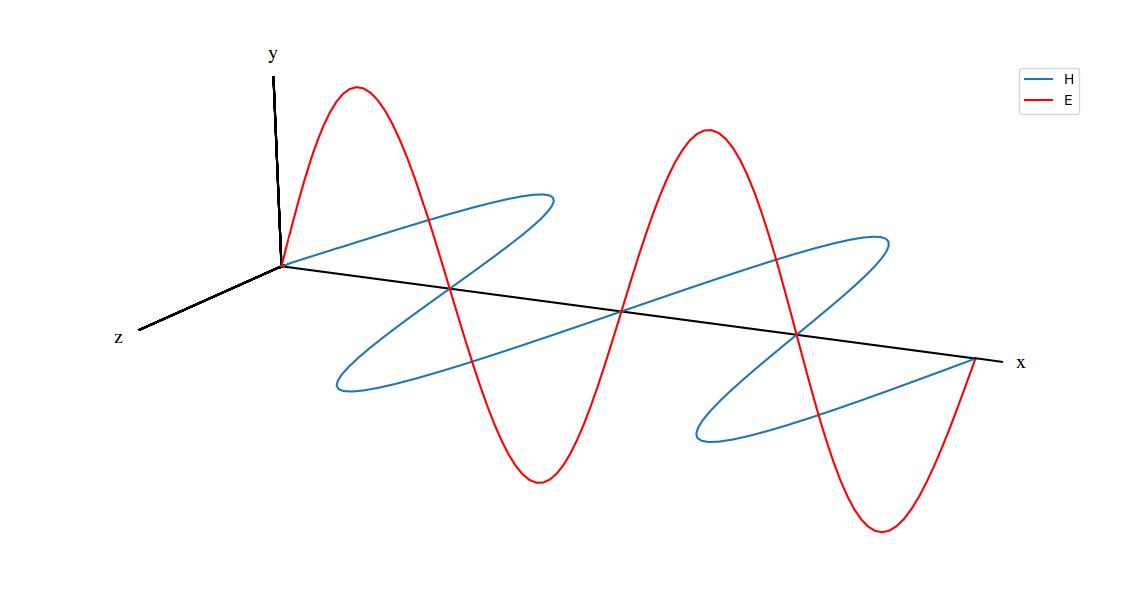
\includegraphics[scale=0.3]
			{images/fig2.png}
	\end{center}
	\centering
	\fautor
\end{figure}

\subsection{Light Wave Properties and Phenomena}

The light waves can be represented by a ray, i.e. a single oriented line which shows the direction of propagation; several waves that propagate in nearly the same direction can be named as a beam \cite{halliday2013fundamentals}. 

% These two models of the real light are important and useful representations within the boundaries of visible light, and allow easier explanations of light properties.

Some relevant properties of waves are explained here according to \citeonline{tipler2007physics}. The frequency ($f$) is the number of cycles per unit of time, or the reciprocal of the time that a periodic wave takes to execute a complete cycle of oscillatory motion $T$, given by $f = T^{-1}$. The Amplitude is the maximum displacement from the equilibrium position, where the wave peak reaches its highest value. Finally, the Phase is a point in time on the cycle of a wave propagation, quantified in degrees.

When rays or beams of light reach surfaces during its propagation, there are four prominent phenomena to consider: reflection, refraction, interference and diffraction. The incident ray of light suffers a split procedure when it reaches a frontier between two homogeneous media. One of the resulting rays reflects within the initial medium and the other one propagates inside the other medium; the first phenomenon is denominated \emph{reflection} and the second, \emph{refraction} \cite{born1999principles}. The speed of light depends on the medium in which it propagates. The \emph{refractive index} is a number that quantifies the speed of light in a particular medium in relation to the speed of light in vacuum, and can be described by

\begin{equation}
    \label{eqn:refractive_index}
       n = \frac{c}{v},
\end{equation}

\noindent where $\mathit{c}$ is the speed of light in vacuum and $\mathit{v}$ is the speed of light in the medium. According to \citeonline{halliday2013fundamentals}, the reflection law states that the resulting ray propagates within the incidence plane and that the angle of reflection $\mathit{\theta^{'}_{1}}$ equals the $\mathit{\theta_{1}}$ angle of incidence; comparably, the refraction law states the same about the incidence plane and relates the incidence $\mathit{\theta_{1}}$ and refraction $\mathit{\theta_{2}}$ angles by Snell's law, given by

\begin{equation}
    \label{eqn:snells_law}
       n_{2}\sin{\theta_{2}} = n_{1}\sin{\theta_{1}},
\end{equation}

\noindent where $\mathit{n_{1}}$ and $\mathit{n_{2}}$ are the refractive indices of the media. This framework consists of an approximation and may be considered ideal for didactic purposes. The process that happens in the real situations may involve non-homogeneous media, opaque or translucent media (which blocks the propagation of light or randomly changes the direction of the rays, respectively), and those concepts are relevant to the imaging procedures, e.g. microscopy. \autoref{fig:beam_split} depicts the real-world phenomenon and its ideal representation.

\begin{figure}[htb]
	\centering
	\caption{\label{fig:beam_split} 
	    (a) Example of a beam of light that reflects and refracts when touching the frontier between air and water. (b) Representation of the process with rays.}
	\begin{center}
	    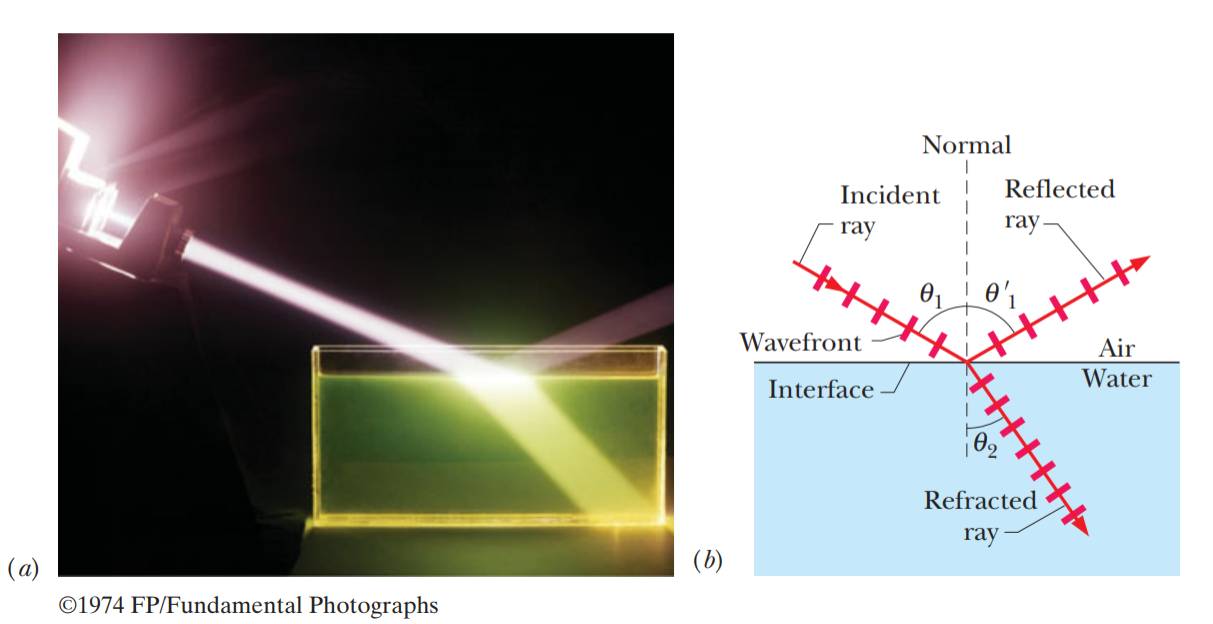
\includegraphics[scale=0.3]{images/fig3.png}
	\end{center}
	\centering
    \fdireta{halliday2013fundamentals}
\end{figure}

When two or more waves of similar or equal frequency superpose in space and form a different intensity pattern, the \emph{interference} of the waves occurred \cite{tipler2008physics}. Mathematically, when interference is observed with light waves, it consists on a vector addition of the electromagnetic fields \cite{zilio2009optica}.
If the interfering waves are in phase, i.e. the difference between the same positions within the wave cycles of the two waves is zero. This process is called \emph{constructive}, which yields a larger amplitude to the new wave. Similarly, if the interfering waves are not in phase, then the process is named \emph{destructive} and yield smaller or null amplitudes to the new wave \cite{tipler2007physics}. Both types of interference are show in \autoref{fig:interference}.

\begin{figure}[htb]
	\centering
	\caption{\label{fig:interference} 
	    (a) Constructive interference and (b) destructive interference.}
	\begin{center}
	    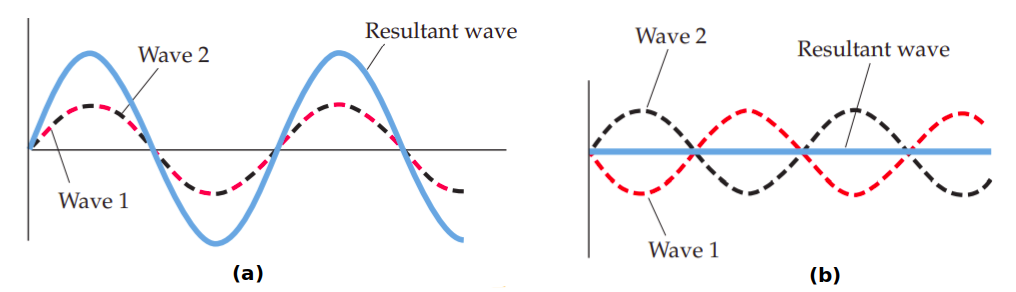
\includegraphics[width=\textwidth,height=4cm, trim=1 1 1 1,clip]{images/interference.png}
	\end{center}
	\centering
    \fadaptada{tipler2007physics}
\end{figure}

The wave theory of light also contains another important property for the real processes: the \emph{diffraction}, a phenomenon that was discovered by Francesco Maria Grimaldi (1618-1663) and consists of the distortion in a wavefront which focuses on obstacles such as apertures on an object, spheres, disks, or anything with similar dimension to the wavelength of the focusing light \cite{zilio2009optica}. The wavefront deviates and scatters after propagating through the obstacle and transforms itself into circular or spherical waves; this is a relevant property that distinguishes a wave from a particle, since the latter would either propagate without any change in its trajectory or would be blocked by the obstacle \cite{tipler2007physics}. When a beam of light reaches an opaque object, the waves suffer changes in their direction of propagation, which can be predicted by the fact that all the points in each wavefront (points of identical phase on waves) generate a new wave, as stated by Huygens \cite{fowles1989introduction}. As described by the Huygens principle, each point of the wavefront acts as a source and creates secondary waves which scatter in every direction; each of the new wavefronts is generated by the interference of an infinite number of sources of waves \cite{zilio2009optica}. The scheme in \autoref{fig:diffraction} illustrates the diffraction phenomenon with an arbitrary obstacle and a small source of waves.

\begin{figure}[htbp]
	\centering
	\caption{\label{fig:diffraction} Diffraction scheme of a wavefront.}
	\begin{center}
	    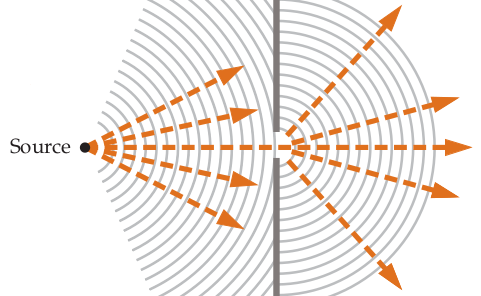
\includegraphics[scale=1.9]{images/diffraction.png}
	\end{center}
	\centering
    \fdireta{tipler2007physics}
\end{figure}

Diffraction is a phenomenon that always happens as waves pass through apertures, but its magnitude depends on the relative proportions between the aperture size and the wavelength: when the latter is large in comparison to the former, the diffraction effects are large and, likewise, a relatively small wavelength yields smaller effects \cite{tipler2007physics}. As stated by \citeonline{zilio2009optica}, there are two common types of diffraction:

\begin{itemize}
    \item \emph{Fresnel Diffraction}: also named near-field diffraction, it occurs when a cylindrical wavefront (the curvature cannot be neglected) passes through an obstacle and diffracts in the near-field, i.e. short distances relative to the path of the diffracted waves' propagation. However, the observation distance is usually finite. It results in different sizes and shapes for the diffraction patterns;
    
    \item \emph{Fraunhofer Diffraction}: also named far-field diffraction, it occurs when planar waves (the curvature of the wavefront may be neglected) pass through an obstacle in the far-field, i.e. large distances relative to the path of the diffracted waves' propagation. Practically, the observation distance is infinite. It results in different sizes for observed aperture images.
    
\end{itemize}

\subsection{Illumination Qualities}

The propagating waves, rays or beams of light that illuminate the object in imaging systems carry some attributes which depend on the source and the desired result. \autoref{fig:illumination_qualities} depicts some relevant qualities of light. 


\begin{figure}[htb]
	\centering
	\caption{\label{fig:illumination_qualities} Comparison between different qualities of an imaging systems' illumination setup.}
	\begin{center}
	    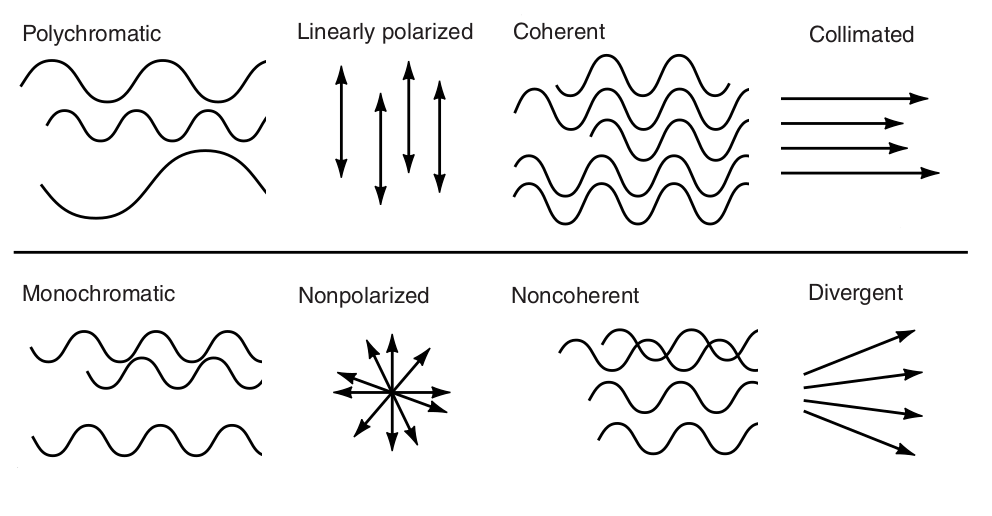
\includegraphics[scale=0.4]{images/light_qualities.png}
	\end{center}
	\centering
    \fadaptada{murphy2012fundamentals}
\end{figure}

Pursuant to \citeonline{murphy2012fundamentals}, the attributes in \autoref{fig:illumination_qualities} 
refer to color, polarization, coherence and direction. Every ray in a \emph{monochromatic} beam has the same wavelength, i.e. the same color, and similarly a \emph{polychromatic} beam consists of a mixture of rays with different wavelengths. The polarization relates to the vibration in the electric vector of light as an electromagnetic wave which may occur in parallel planes (\emph{polarized light}) or not (\emph{nonpolarized light}). The coherence is the relationship between the phase of each wave of a given wavelength: if the phase is the same for all waves, as in a laser beam, the light is named \emph{coherent}, otherwise it is said that the illumination is \emph{noncoherent} or \emph{incoherent}, as in bright-field microscopes. Finally, the waves may propagate in parallel trajectories, i.e. be \emph{collimated}, or may diverge or converge to some point.

\subsection{Properties of the Spherical Lenses}

As stated by \citeonline{halliday2013fundamentals}, \emph{lenses} are objects consisting of a transparent material, with a certain refractive index, that are made of two spherical surfaces on which light propagates and suffers refraction. They are used in optical systems due to their capacity to create images as long as their refractive index is not equal to that of the medium. Yet, in agreement with \citeonline{halliday2013fundamentals}, some concepts related to lenses are important in our context and will be shown below. \autoref{fig:spherical_lens} illustrates an arbitrary spherical lens, with principal elements from geometric optics that relate to lenses and its consequent imaging properties.

\begin{figure}[htb]
	\centering
	\caption{\label{fig:spherical_lens} Arbitrary scheme of the optical properties of a spherical lens: radii of curvature ($r_{1}$, $r_{2}$), centers of curvature ($C_{1}$, $C_{2}$), focal points ($F_{1}$, $F_{2}$) and focal length ($f$).}
	\begin{center}
	    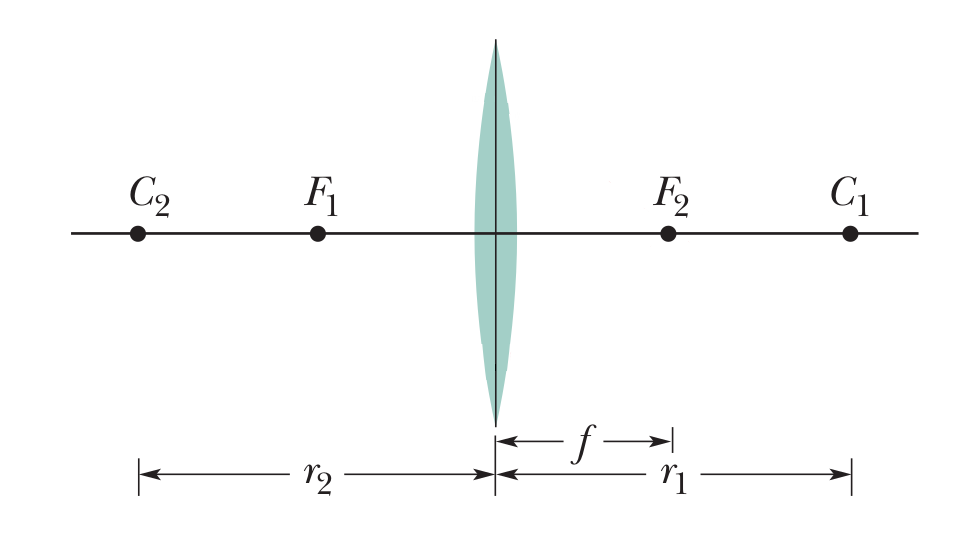
\includegraphics[scale=0.4]{images/fig4.png}
	\end{center}
	\centering
    \fadaptada{halliday2013fundamentals}
\end{figure}

Some properties of the spherical lenses directly influence the image formation process and, consequently, the resulting image quality. The \emph{numerical aperture} (NA), as reported by \citeonline{murphy2012fundamentals}, is a measurement in terms of angles that shows how much light the lenses can capture, and it is given by

\begin{equation}
    \label{eqn:numerical_aperture}
    NA = n \sin{\theta},
\end{equation}

\noindent where $\theta$ is the half angle of the cone of specimen light accepted by the objective lens and $n$ is the refractive index between the lens and the specimen. There are optical flaws in lenses that hinder a proper image formation. Those are named \emph{aberrations} \cite{lawlor2019introduction}, and the most relevant types in the scope of this project are the \emph{spherical aberrations}. According to \citeonline{murphy2012fundamentals}, the spherical aberrations occur when there is a difference in the focal point of incident parallel rays at central and peripheral locations of a spherical lens' surface, which yields a blurred image of either a point source of light or an extended object. It is possible to correct a spherical aberration by changing the shape of the refracting surface, i.e. changing the radius of curvature for the lenses in order to adjust the focal point to one particular distance \cite{smith1988optics}. The illustration in \autoref{fig:spherical_aberrations} represents the spherical aberration for a point source of light, where it is possible to see the difference between incident rays in the borders and in the inner regions of the lens. The resulting image is, in this case, a set of concentric circles around a point.

\begin{figure}[htb]
	\centering
	\caption{\label{fig:spherical_aberrations} Arbitrary example of the spherical aberration.}
	\begin{center}
	    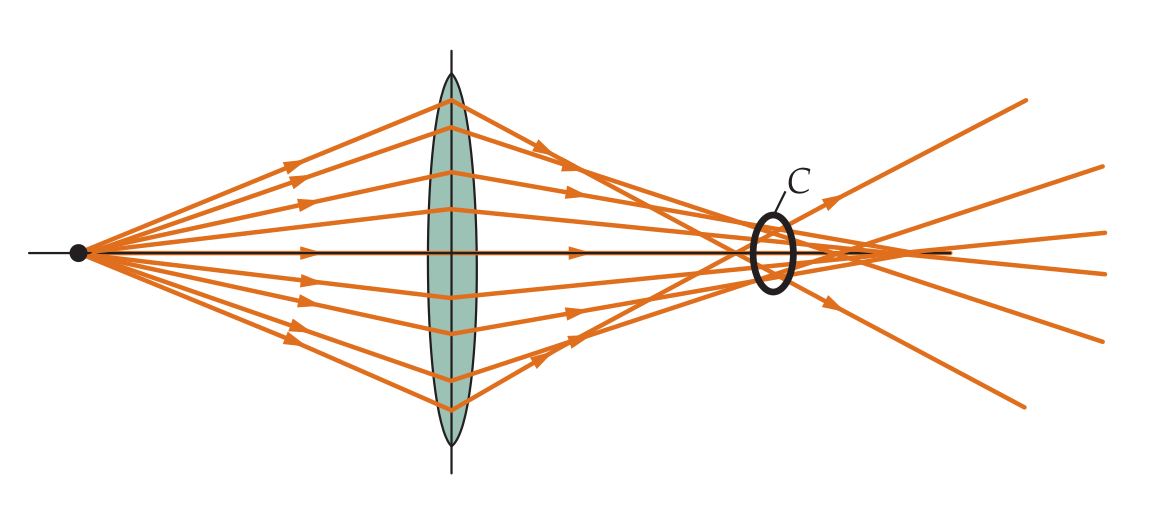
\includegraphics[scale=1.5]{images/spherical_aberration.png}
	\end{center}
	\centering
    \fdireta{tipler2008physics}
\end{figure}

\vspace{-1cm}
    
    \chapter{Theoretical Background Details}
    \label{chapter:theoretical-background-details}
    \section{Convolution and Image Transforms}

As seen in Chapters \ref{chapter:fundamentals-of-optics-and-light-microscopy} and \ref{chapter:blur-characterization-and-image-formation}, the processes of image formation and acquisition concerning linear systems are subject to some operations, i.e. the convolution, the \sigla{FT}{Fourier Transform} and its continuous and discrete versions, that modify the original representation of the scene. The linear system theory provides mathematical tools to explore these operations and others, such as sampling, filtering, and enhancement; it describes the behavior of electrical circuits and optical systems \cite{castleman1996digital}.

According to \citeonline{bracewell2000fourier}, the convolution of two arbitrary functions $s$ and $t$ that results in another function $r$ is, with notation adjustments, defined by the integral

\begin{equation}
\label{eqn:one_dimensional_convolution}
r(x) = \int_{-\infty}^{\infty}s(u) t(x - u) du,
\end{equation}

\noindent where $x$ is the one-dimensional coordinate and $u$ is a shifting parameter. In other words, this procedure is compared to moving a 180 degree-rotated filter mask over the function values and computing the sum of products at each location \cite{gonzalez2018digital}. Hence, the shifting parameter represents the slide of the filter mask over the values. As seen in \autoref{chapter:blur-characterization-and-image-formation}, convolution is responsible for the image formation and acquisition processes, but it also covers several other applications, e.g. smoothing, sharpening and reducing noise in images. Similarly to the one-dimensional case and pursuant to \citeonline{castleman1996digital}, the two-dimensional convolution is denoted by

\begin{equation}
\label{eqn:two_dimensional_convolution}
r(x,y) = \int_{-\infty}^{\infty}
         \int_{-\infty}^{\infty}
         s(u,v) t(x - u, y - v) du dv,
\end{equation}

\noindent where $u$ and $v$ are shifting parameters, and $\ast$ denotes the convolution. The \emph{spatial domain} is the subset of the real plane where functions like $r$, $s$ and $t$ are spanned, and $(x,y)$ as points within such subset are named spatial variables; consequently, any mathematical operation that employs pixels from this subset is named a spatial domain technique. As for the digital image processing applications, which deal with images as matrices of pixels, the discrete two-dimensional convolution for an image $f(x,y)$ and a function $h(x,y)$ is given by 

\begin{equation}
\label{eqn:2d_discrete_convolution}
g(x,y) = h(x,y) \ast f(x,y) = 
        \sum_{m=-a}^{a}
        \sum_{n=-b}^{b}
        f(m,n) h(x-m,y-n),
\end{equation}

\noindent where $a = (m-1)/2$ and $b = (n-1)/2$, given that the function $h(x,y)$ is considered to be a two-dimensional filter of size $m \times n$ \cite{gonzalez2018digital}.

Convolution, together with several other operations employed in this work, operate directly on the spatial domain by modifying pixel values based on mathematical constraints. Some of those operations may have issues that hinder the operation, e.g. the computation time of a convolution process should be finite, otherwise, its use is impractical; this is one of the reasons why \emph{image transforms} are widely used. They encompass any group of mathematical operations that transfers the input signal or image from its domain to the transform domain \cite{gonzalez2008digital}. Let $s$ be an arbitrary two-variable function, $t_{f}$ and $t_{i}$ be the forward and inverse transformation kernels, respectively. The general discrete form of the forward and inverse two-dimensional transforms is denoted by 

\begin{align}
\label{eqn:generic_transform}
R(u,v) = 
\sum_{x=0}^{M-1}
\sum_{y=0}^{N-1}s(x,y)t_{f}(x,y,u,v)
&&
s(x,y) = 
\sum_{x=0}^{M-1}
\sum_{y=0}^{N-1}R(u,v)t_{i}(x,y,u,v),
\end{align}

\noindent where $M$ and $N$ are the dimensions of the image, $x$ and $y$ are coordinates of the image, $u = \{0,1,2,...,M-1\}$ and $v = \{0,1,2,...,N-1\}$ are called transform variables. The $t_{f}$ function is responsible for the forward domain change and the $t_{i}$ transfers the image back to the spatial domain. Switching from spatial to frequency domain, for example, allows different operations to be executed that otherwise could not be performed in the spatial domain. The convolution operation, for instance, turns itself into a simple matrix multiplication task on the Fourier Transform domain (which will be detailed in the following sections) and that solves the performance constraint.

\section{Image Enhancement}

Image enhancement is the process of manipulating an image in order to provide a resulting representation that is more suitable for a particular problem, e.g. an enhancement method for medical images may not be efficient for satellite images \cite{gonzalez2018digital}. In microscopy, image enhancement is desirable due to the limited capacity of optical imaging devices and the drawbacks posed by each microscopy technique, e.g. acquisition with different illumination settings, focal planes, time intervals or spectral channels. Therefore, enhancement algorithms for microscopy should cover all types of information \cite{wu2008microscope}. According to \citeonline{wu2008microscope}, image enhancement techniques are divided into \emph{spatial domain}, \emph{Fourier transform} and \emph{wavelet transform} methods. They will be described in the following paragraphs. 

The spatial domain methods are transforms that work directly on pixels of the image \cite{gonzalez2018digital}. Some examples are contrast stretching (redistribution of image gray levels to a wider range), thresholding (image binarization given a preset gray level), histogram equalization, and spatial filtering. Particularly, histogram equalization and spatial filtering play an important role in this work and therefore will be explored further.

Fourier transform domain methods operate with images as a distribution of frequencies since some features are better described by it. Noise, for example, may be suppressed in a sharpening process or reduced by amplifying mid-frequency components and attenuating high-frequency ones. The Wiener Filtering process is a popular example of a frequency domain enhancement method that recovers a noisy signal or image based on estimations of spectral properties from the original image. Other examples of Fourier domain enhancement are band-pass filters and least-squares deconvolution applications. 

Finally, there are methods based on the Wavelet Transform, i.e. a mathematical framework that decomposes images or signals into frequency components in different scales. Some operations such as thresholding may be applied to wavelet coefficients. However, the output of the wavelet transform is not always the same; it depends on the chosen wavelet function and consequently should be properly set in order to extract the desired image features.

The image histogram is one of the simplest and most useful tools in image processing and consists of a function that summarizes the gray level content of an image in terms of a frequency distribution \cite{castleman1996digital}. The histogram equalization consists of a non-linear monotonic mapping to provide an approximation of a uniform distribution to the output image's histogram \cite{gonzalez2018digital}. The output histogram is a normalization of the cumulative histogram of the image, given by

\begin{equation}
\label{eqn:histogram_equalization}
hist_{equalized}(r) = \frac{L - 1}{MN} hist_{cumulative}(r),
\end{equation}

\noindent where $hist_{equalized}(r)$ and $hist_{cumulative}(r)$ are the equalized and cumulative histograms relative to a range $L$ of intensities after the image quantization with $r$ values. $M \times N$ is the image resolution. Since it stems from a sum of probabilities and no new gray intensity levels should be created, the process generates fractional values that are mapped onto integers.

Spatial filtering consists of the convolution of an image with a predefined kernel operator \cite{gonzalez2018digital}. The continuous form may be represented as a convolution over all values of a defined region of the image and the discrete form consists of sliding a weight mask over the image \cite{wu2008microscope}. \autoref{fig:generic_spatial_filtering} presents an arbitrary schema of a simple linear spatial filtering procedure:

\begin{figure}[htb]
	\centering
	\caption{\label{fig:generic_spatial_filtering} Arbitrary example of linear spatial filtering of an image (a) with a $3 \times 3$ filter mask (b), which results in filtered sections (c).} 
	\begin{center}
	    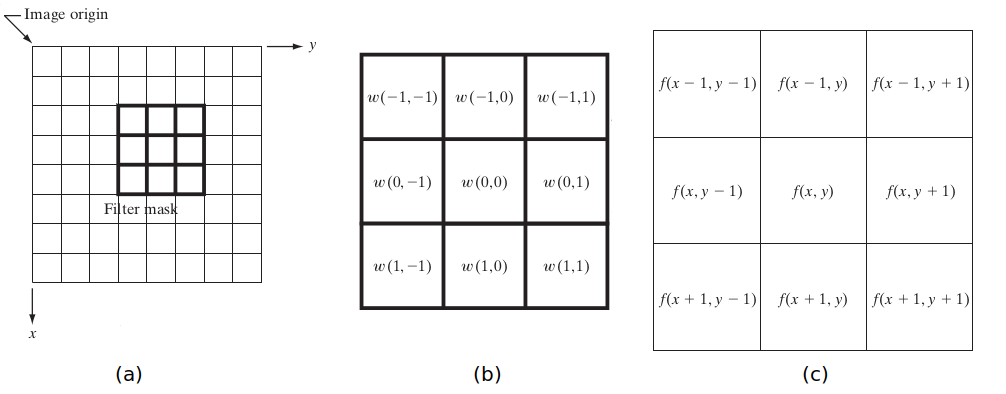
\includegraphics[scale=0.4]{images/generic_spatial_filtering.png}
	\end{center}
	\centering
    \fadaptada{gonzalez2018digital}
\end{figure}

Examples of discrete spatial filtering in digital image processing are smoothing filters, order-statistic nonlinear filters and sharpening filters \cite{gonzalez2018digital}. Spatial smoothing filters are applied to remove details, edges and lines from an image to reduce noise. The order-statistic nonlinear filters are based on ordering pixels of the image under the filter area and replacing the pixel value in the center of the area with the response from ordering; one example is the \emph{median filter}, which replaces the center pixel with the median of pixels in its neighborhood. Median filters yield significant noise reduction effects if the nature of the noise is random. Finally, the sharpening filters are built to highlight transitions in intensity by spatial differentiation and are used for enhancing edges.

\section{Image Registration}

When images belonging to the same scene are acquired in different conditions such as distinct focus configurations, sensors, or even at different times, they should be geometrically aligned according to a reference image. The process of overlaying two or more images with different acquisition settings is named image registration and plays an important role as a pre-processing step for image fusion, change detection and multichannel image restoration \cite{zitova2003image}. According to \citeonline{gonzalez2018digital}, magnetic resonance imaging and positron emission tomography systems, for example, are two different medical image modalities that may require images to be registered. Images which were taken in different times such as satellite images also need to be registered.

The image registration methods consist of the following steps, as reported by \citeonline{zitova2003image} and \citeonline{gonzalez2018digital}:

\begin{itemize}
    \item \emph{Feature detection}: manually or automatically detect distinctive objects, e.g. edges, contours, corners and represent those as \emph{control points}, i.e. points with known locations in the reference and input images;

    \item \emph{Feature matching}: a relationship between the detected features in each image is established using feature descriptors;

    \item \emph{Transform model estimation}: parameter estimation for mapping functions that align the input images with the reference image, either by establishing feature correspondence or performing an optimization procedure;

    \item \emph{Image resampling and transformation}: the image is resampled with interpolation techniques.

\end{itemize}

Image registration is, in practice, a mapping between two or more images by means of a spatial and an intensity transformation \cite{brown1992survey}. Some prominent examples of registration methods are the principal axes, multiresolution, optimization-based, boundary, model-based and adaptive methods  \cite{goshtasby2012image}. The spatial transformations play an important role in all image registration techniques, and the most common examples are rigid, affine, projective, perspective and global polynomial \cite{brown1992survey}. Also pursuant to \citeonline{brown1992survey}, each of such transformations may be described as:

\begin{itemize}
    \item \emph{Rigid}: accounts for object or sensor movement in which objects in the images retain their relative shape and size. Example: \emph{rigid-body transformation} which combines rotation, translation and scale changes; 
    
    \item \emph{Affine}: handle more complicated distortions and preserve mathematical properties. Example: \emph{shear transformation};
    
    \item \emph{Projective and Perspective}: the former deals with distortions due to projection of the objects at varying distances to the sensor onto the image plane, and the latter demands prior knowledge about the locations of the objects in the scene relative to the sensor;
    
    \item \emph{Polynomial}: cover the broadest range of distortions, as long as they are approximately homogeneous in the image.
\end{itemize}

\section{Image Fusion}
Image fusion is a process that merges several images, possibly acquired in diverse conditions or with different cameras, into one image with higher quality, more details and consequently more useful for humans and computer tasks \cite{mitchell2010image}. Examples of image fusion applications are noise reduction, edge enhancement, and super-resolution. One traditional use of image fusion occurs in medical imaging fields; the quality of information about illnesses, cells, clinical analysis and several other medical tasks (including the computer-assisted ones) have found profitable results from the image fusion techniques and led themselves to better and faster decisions when it comes to human beings \cite{james2014medical}. There are also relevant applications in remote sensing multispectral images, segmentation of regions in different color spaces, biometry: the pan-sharpening process is the generation of a high-resolution multispectral image from low to high-resolution ones, K-Means segmentation and fusion of pixels in the RGB and the Iris Recognition biometric process with video frames are examples of such tasks, respectively \cite{mitchell2010image}.


Also according to \citeonline{mitchell2010image}, the general framework for the image fusion procedure consists of four stages: \emph{Multiple Input Images}, \emph{Common Representational Format}, \emph{Fusion} and \emph{Display}.
The multiple input images stage is simply the acquisition of the images to be merged. There are several approaches to this: the dataset may be captured from different sensors, under distinct light conditions or angles, with different magnifications, under several focus settings, and with temporal measurements, if the scene changes through time.

If the acquired dataset images do not share the same features such as dimension, rotation angle, and resolution, then the images should be pre-processed in order to arrive at a common state. This configures the common representational format step, which generates a new and temporary dataset with the same properties, e.g. color space, dimensions, and noise level. The fusion stage employs a decision method to dictate which regions, objects, colors or details will compose the final image; some methods rely on the wavelet transform, for example. Finally, the display stage provides a view of the resulting image, which can be used directly for any further task or even be the input for other image processing operations. \autoref{fig:fusion_general_framework} depicts an arbitrary example of the four stages. 

\begin{figure}[ht]
	\centering
	\caption{\label{fig:fusion_general_framework}Image fusion general framework. (a) Multiple Input Images, (b) Common Representational Format, (c) Fusion and (d) Display.}
	\begin{center}
    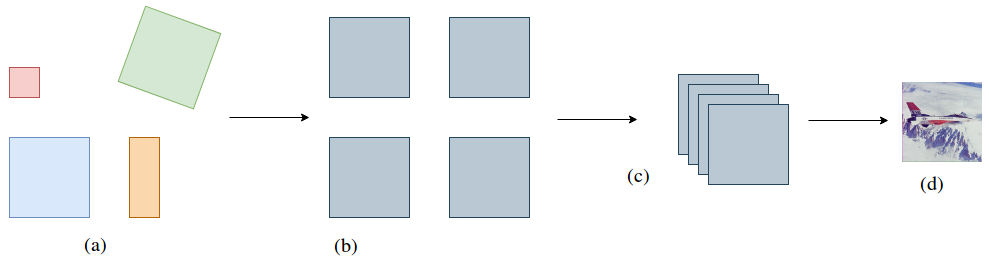
\includegraphics[scale=0.45, trim={0 -1.5cm 0cm -1.5cm}, clip]{images/image_fusion_scheme.png}
	\end{center}
	\centering
    \fautor
\end{figure}

The four arbitrary images in \autoref{fig:fusion_general_framework}.\textbf{(a)} represent different images of the same scene, taken at different resolutions, rotation angles, and shapes. In \autoref{fig:fusion_general_framework}.\textbf{(b)}, the images are all reshaped, converted to common color space and ready to undergo the processing algorithm which will transform them into feature vectors. \autoref{fig:fusion_general_framework}.\textbf{(c)} represents the image fusion by means of an arbitrary fusion rule. The resulting image is depicted in \autoref{fig:fusion_general_framework}.\textbf{(d)}. Since image fusion is only one branch of data fusion field, this procedure has a wide variety of approaches and methods; hence, the domain will be restricted to the multi-focus image fusion and some relevant related work will be presented in \autoref{chapter:related-work}.

\section{Image Quality Assessment}
\sigla{IQA}{Image Quality Assessment} is the evaluation of image quality as perceived by an average human observer, i.e. how close an image is to a given original or reference image. It is also related to the accuracy of the image acquisition process for an imaging system \cite{bovik2009essential}. It is known that images are frequently used in health and life sciences, public security systems, remote sensing, and several other fields; hence, there are computational applications that offer some useful service employing image processing. As a result, assessing image quality poses as an important task among those applications for which several techniques are being developed, evolved and deployed.

According to \citeonline{tang2019feature}, the IQA methods are distributed between the subjective assessment and objective assessment categories. The former is based on a well-defined test environment for random observers to label images and provide the final \sigla{MOS}{Mean Opinion Scores}, while the latter is based on the use of strategies such as statistical modeling, machine learning, spatial or spectral image features and so on. It is evident that subjective IQA is demanding; consequently, objective methods are preferred to conduct IQA.

According to \citeonline{wang2004image}, there are three classes of objective image quality metrics that relate to the existence of a no-distortion image (or with a negligible amount of it) for comparison purposes. The \sigla{FR-IQA}{Full-Reference Image Quality Assessment} methods assume that the reference image is available, while \sigla{RR-IQA}{Reduced-Reference Image Quality Assessment} methods employ a representation of the reference image, such as a set of extracted features. Finally, the \sigla{NR-IQA}{No-Reference Image Quality Assessment} methods, also known as ``blind'', are those which do not employ a reference image. \autoref{fig:mssim_IQA_exampe} denotes an example of a full-reference method, the \sigla{MSSIM}{Mean Structural Similarity Measure} method and its output for an image with different types of degradation:

\begin{figure}[ht]
	\centering
	\caption{\label{fig:mssim_IQA_exampe} Example of the MSSIM method output: Original image (a), contrast-stretched image (b), mean-shifted image (c), JPEG compressed image (d), blurred image (e) and salt-pepper impulsive noisy image (f).}
	\begin{center}
    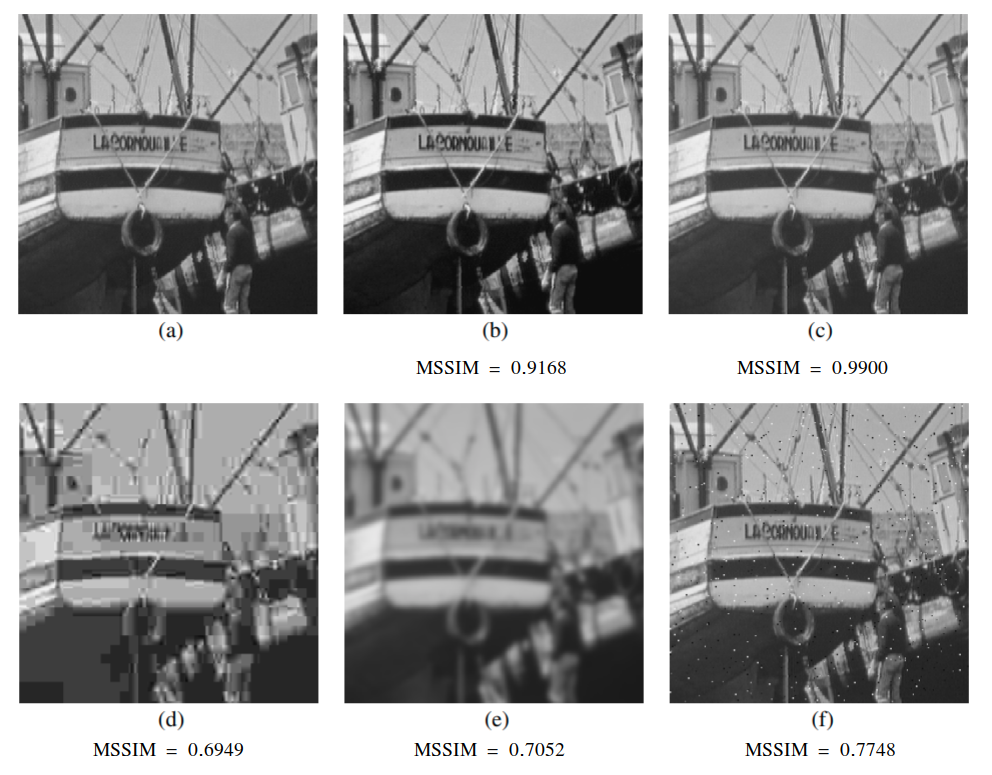
\includegraphics[scale=0.4]{images/mssim_IQA.png}
	\end{center}
	\centering
    \fdireta{wang2004image}
\end{figure}

IQA methods are also present within microscopy and its close interaction with image processing. The image acquisition in microscopy techniques may involve lasers, transmitted or reflected light, measurements of atomic force responses, the fluorescence of chemical compounds and several other means. Each technique has an inherent kind of degradation that affects the acquired images or spectra, e.g. the Raman confocal microspectroscopy suffers from the interference of cosmic rays, which yields unexpected peaks in the spectrum. Therefore, the use of IQA methods is expected. They will be investigated and used in this work. In \autoref{chapter:related-work}, some examples of NR-IQA techniques that guided the development of our method will be presented.

\section{Statistics}

Statistics is the science of planning studies and experiments, obtaining, organizing, summarizing, presenting, analyzing, and interpreting data and finally drawing conclusions. \emph{Descriptive statistics} is an important branch that comprises a set of methods which aim to describe relevant characteristics in data \cite{triola2017elementary}. The descriptive statistics methods either employ graphical elements such as boxplots, histograms, bar graphs and scatter plots to analyze data or yield numerical summary measures such as means, standard deviations, correlation coefficients and other related indices \cite{devore2011probability}. The methods that compose a descriptive statistical approach for data analysis are simple yet powerful tools.

The concepts of \emph{population}, \emph{sample} and \emph{variable} are elementary: a population is a well-defined collection of objects that might be included in the analysis, a sample is a subset of a population and a variable is a feature of the objects which may change from one object to another \cite{devore2011probability}. Moreover, a \emph{frequency distribution} is a tool that presents how the data is partitioned among several categories by listing each category and its frequency of data values; a \emph{relative frequency distribution} is a frequency distribution in which each frequency is represented by a proportion, usually as percentage \cite{triola2017elementary}. According to \citeonline{mendenhall2016statistics}, the measures of central tendency provides several ways to locate the center of the relative frequency distribution, and the three most common are the \emph{arithmetic mean}, i.e. the average of the measurements, the \emph{median}, i.e. the middle number when the measurements are ordered in ascending or descending order and the \emph{mode}, i.e. the value that occurs with the greatest frequency. Mathematically, the arithmetic mean is given by

\begin{equation}
\label{eqn:arithmetic_mean}
\bar{x} = \frac{1}{n} \sum_{i=1}^{n} x_{i} = \frac{x_{1} + x_{2} + \dots + x_{n}}{n},
\end{equation}

\noindent where $n$ is the sample size and $x_{i}$ represents the $i$-th observation of the variable $x$ \cite{zwillinger1999crc}.

% \subsection{Measures of Variation}

The measures of variation provide a description of how the values spread along the distribution. Commonly used measures are the range, the variance, and the standard deviation \cite{mendenhall2016statistics}. The range is simply the difference between the largest and the smallest value within the data, which may precisely point out its variability, since it does not comprise the middle values among the distribution \cite{devore2011probability}. The variance and the standard deviation are closely related, as the former measures variability based on the squared deviations about
the mean and the latter is the positive square root of the variance, as

\begin{align}
\label{eqn:variance_std}
\sigma^{2} = \frac{1}{n - 1} \sum_{i = 1}^{n} \left(x_{i} - \bar{x}\right)^{2}
&&
\sigma = \sqrt{\sigma^{2}}
\end{align}

\noindent where $\sigma^{2}$ and $\sigma$ are respectively the variance and the standard deviation, $x_{i}$ is the $i$-th observation of the variable $x$, $\bar{x}$ is the mean, all concerning a sample or the population \cite{zwillinger1999crc}.

% \subsection{Measures of Relative Standing and Outlier Detection}

The measures of the relative standing of an observation describe its location among other values in the distribution, and two examples of these measures are \emph{percentiles} and \emph{z-scores}; also, an observation located outside the range of the distribution is an \emph{outlier} \cite{mendenhall2016statistics}. Percentiles are values that split the data into 100 parts in a sorted dataset, so that the $i$-th percentile stands for the $i(n + 1) / 100$ observation, e.g. the $25$-th percentile comprises $25\%$ of the data; the $z$-score, or standard score, is given by

\begin{equation}
\label{eqn:z_score}
z = \frac{x_{i} - \bar{x}}{\sigma},
\end{equation}

\noindent where $x_{i}$ is the $i$-th observation of the variable $x$, $\bar{x}$ is the mean and $\sigma$ is the standard deviation of the population or the sample \cite{zwillinger1999crc}. 

The Interquartile Range (IQR) is the length of the interval that contains the middle half of the distribution \cite{degroot2012probability}. Mathematically, it is the difference between the third ($Q_{3}$) and the first ($Q_{1}$) quartiles, i.e. the $75$th percentile $25$th percentile, respectively \cite{devore2011probability}. The IQR is described by

\begin{equation}
\label{eqn:iqr}
IQR = Q_{3} - Q_{1}.
\end{equation}

% \subsection{Probability Distributions}

Probability is a common and natural concept among human life, used in expressions such as ``It probably will be cold tonight''; however, there is no common formal definition accepted among statisticians and related researchers \cite{degroot2012probability}. The study of randomness, variability and uncertainty in populations is done by analyzing probabilities, i.e. numerical descriptions of how likely an event is to occur \cite{devore2011probability}. Some basic concepts that support the probability theory are described also to the light of \citeonline{devore2011probability}, as follows:

\begin{itemize}
    \item \emph{Experiment}: any activity or process whose outcome is subject to uncertainty;
    
    \item \emph{Sample Space}: the sample space of an experiment is the set of all possible outcomes for it;
    
    \item \emph{Event}: any collection or subset of outcomes of a sample space;
    
    \item \emph{Random Variable}: any rule that associates a number with each outcome in a sample space of some experiment; mathematically, it is a function with the sample space as its domain and the real numbers as its range;
    
    \item \emph{Discrete Random Variable}: a random variable with a finite set or a countable infinite sequence of possible values;
    
    \item \emph{Continuous Random Variable}: a random variable that yields zero as the probability for every possible outcome or its set of possible values are in a single interval of the real line or all numbers in a disjoint union of intervals.
    
\end{itemize}

From these concepts, it is possible to define a distribution in the scope of the probability theory. The \emph{probability distribution} is a collection of all probabilities computed from a  discrete or continuous random variable with the set of real numbers; a \emph{discrete} probability distribution is represented by the probability function itself, while a \emph{continuous} probability distribution is represented by a \sigla{p.d.f}{probability density function} \cite{mendenhall2016statistics}.


The \emph{kurtosis} is one of the probability distribution shape statistics, which measures the extent of the peak in a distribution, i.e. its ``peakedness''; smaller absolute values indicate that the distribution tends to be uniform \cite{zwillinger1999crc}. First of all, the concepts of \emph{expectation} and \emph{moments} should be described. The expectation of a random variable (and consequently, of a distribution) is a value that summarizes its nature and is given by

\begin{align}
\label{eqn:expectation}
E(X) = \int_{-\infty}^{\infty} x p(x)dx
&&
E(X) = \sum_{x} x p(x),
\end{align}

\noindent where $x$ is each possible outcome of the random variable $X$, $p(x)$ is the probability density function for a continuous random variable (left) and the probability function for a discrete random variable (right) \cite{degroot2012probability}. Still according to \citeonline{degroot2012probability}, for a random variable $X$ and every positive $k \in \mathbb{R}$, the expectation $E(X^{k})$ is
called the $k$-th moment of $X$. The $r$-th moment may be described, according to \citeonline{zwillinger1999crc}, as

\begin{equation}
\label{eqn:rth_moment}
m_{r} = \frac{1}{n}
        \sum_{i=1}^{k}p_{i}(x_{i} - \bar{x})^{r}
\end{equation}

\noindent for every $x_{i}$ in the possible outcomes of $X$. Thus, kurtosis may be defined as the ratio of the fourth moment (\autoref{eqn:rth_moment} with $r = 4$) by the square of the variance (also \autoref{eqn:rth_moment} with $r = 2$), denoted by

\begin{equation}
\label{eqn:kurtosis}
g_{2} = \frac{m_{4}}{(m_{2})^{2}} - 3
\end{equation}

The $-3$ constant is inherited from Fischer's approach, where the kurtosis of a normal distribution is zero.
    
    \chapter{Definitions and Proofs}
    \label{chapter:definitions-and-proofs}
    This appendix presents the mathematical description of how the feature vectors are built and a proof of the fact that the algorithm yields a probability distribution as the final structure, which allows the use of statistical analysis as the basis of our quality metric. Along with the proof, several definitions and auxiliary theorems that are necessary to the understanding of the proof are described.

\vspace{0.1in}

% Algebra
\theoremstyle{definition}
\newtheorem{definition}{Definition}
\begin{definition}{(Algebra) \cite{folland2013real}}

Let $X$ be a nonempty set. A \textbf{field} or an \textbf{algebra} of sets on $X$ is a nonempty collection $\mathcal{A}$ of subsets of $X$ that is closed under finite unions and complements, as described as follows:

\begin{enumerate}[label=(\roman*)]
    \item if $\{E_{j}\}_{j = 1}^{n} \in \mathcal{A}$, then $\bigcup_{j = 1}^{n}E_{j} \in \mathcal{A}$;
    
    \item if $E \in \mathcal{A}$, then $E^{c} \in \mathcal{A}$.
    
\end{enumerate}
\end{definition}
\vspace{0.1in}

% Sigma-algebra
\begin{definition}{($\sigma$-algebra) \cite{folland2013real}}

A \textbf{$\sigma$-field} or \textbf{$\sigma$-algebra} $\mathcal{M}$ is an algebra that is closed under countable unions.
\end{definition}

\vspace{0.1in}

% Measure
\begin{definition}{(Measure) \cite{folland2013real}}

Let $X$ be a set equipped with a $\sigma$-algebra $\mathcal{M}$. A \textbf{measure} on $\mathcal{M}$ is a function $\mu : \mathcal{M} \rightarrow [0, + \infty]$, such that

\begin{enumerate}[label=(\roman*)]
    \item $\mu(\emptyset) = 0$.
    \item if $\{E_{j}\}_{j = 1}^{\infty}$ is a sequence of disjoint sets in $\mathcal{M}$, then
    
    \[ \mu \left( \bigcup_{j = 1}^{\infty} E_{j} \right) = \sum_{j = 1}^{\infty} \mu(E_{j}). \]

\end{enumerate}

\noindent From (ii), if $E_{j} = \emptyset$ for $j > n$, if $\{E_{1},E_{2},...,E_{n}\}$ are disjoint sets in $\mathcal{M}$, then $\mu \left( \bigcup_{j = 1}^{n} E_{j} \right) = \sum_{j = 1}^{n} \mu(E_{j})$.

\end{definition}
\vspace{0.1in}

% Dirac Measure
\begin{definition}{(Dirac Measure) \cite{ccinlar2011probability}}

Let $(X,\mathcal{M})$ be a measurable space and let $x$ be a fixed point of $X$. For each subset $E$ in $\mathcal{M}$, put

    \[ 
        \delta_{x}(E) = \left\{
        \begin{array}{lr}
            1, & \text{if } x \in E\\\
            0, & \text{if } x \notin E\\
        \end{array}
        \right..
    \]

\noindent Then, $\delta_{x}$ is a measure on $(X,\mathcal{M})$ and is called the \textbf{Dirac measure} sitting at $x$.

\end{definition}
\vspace{0.1in}

% Discrete Measure
\begin{definition}{(Discrete Measure) \cite{ccinlar2011probability}}

Let $(X,\mathcal{M},\mu)$ be a measurable space. Let $D$ be a countable subset of $X$. For each arbitrarily chosen $x \in D$, let $m(x) > 0$ . For $E \in \mathcal{M}$, define

    \[ \mu_{E} =  \sum_{x \in D}m(x)\delta_{x}(E). \]

\noindent Then, $\mu$ is called a \textbf{discrete measure} on $(X,\mathcal{M})$.

\end{definition}
\vspace{0.1in}

% Metric Space
\begin{definition}{(Metric and Metric Space) \cite{folland2013real}}

Let $X$ be a nonempty set. A \textbf{metric} on $X$ is a function $\rho : X \times X \rightarrow [0,\infty)$ such that
    
\begin{enumerate}[label=(\roman*)]
    \item $\rho(x,y) = 0 \Leftrightarrow x = y$;
    
    \item $\rho(x,y) = \rho(y,x)$ for all $x,y \in X$;
    
    \item $\rho(x,z) \leq \rho(x,y) + \rho(y,z)$ for all $x,y,z \in X$.
    
\end{enumerate}

\vspace{0.05in}

A set equipped with a metric is called a \textbf{metric space}.

\end{definition}
\vspace{0.1in}

% Open and Closed Ball
\begin{definition}{(Open and Closed Ball) \cite{folland2013real}}

Let $(X, \rho)$ be a metric space. If $x \in X$ and $r > 0$, the \textbf{open ball} of radius $r$ about $x$ is

\[B(r;x) = \{y \in X : \rho(x,y) < r \}.\]

\noindent In other words, a ball of radius $r$ is the collection of points of distance less than (which makes it \textbf{open}) or equal to (which makes it \textbf{closed}) $r$ from a fixed point $x$ in a metric space \cite{croft2012unsolved}.

\end{definition}
\vspace{0.1in}

% Topology
\begin{definition}{(Topology and Topological Space) \cite{royden1988real}}

Let $X$ be a nonempty set. A \textbf{topology} on $X$ is a family of subsets $\tau \subset \mathcal{P}(X)$, satisfying
    
\begin{enumerate}[label=(\roman*)]
    \item $X \in \tau$ and $\emptyset \in \tau$.
    
    \item if $O_{1}, O_{2} \in \tau$ imply $O_{1} \cap O_{2} \in \tau$ ($\tau$ is closed under finite intersections).
    
    \item if $(O_{i})_{i \in I} \in \tau$, then $\cup_{i \in I}O_{i} \in \tau$ ($\tau$ is closed under arbitrary unions).
    
\end{enumerate}

\vspace{0.05in}

\noindent A \textbf{topological space} $(X, \tau)$ is a nonempty set together with a \textbf{topology} $\tau$ on it. The elements of $\tau$ are called \textbf{open sets} of $X$. 

\end{definition}
\vspace{0.1in}

% Topological Vector Space
\begin{definition}{(Topological Vector Space) \cite{folland2013real}}

A \textbf{topological vector space} is a vector space $\mathbb{V}$ over $\mathbb{K} = (\mathbb{R}$ or $\mathbb{C})$ which is endowed with a topology such that the maps $(x,y) \rightarrow x + y$ and $(\lambda,x) \rightarrow \lambda x$ are continuous from $\mathbb{V} \times \mathbb{V}$ and $\mathbb{K} \times \mathbb{V}$ to $\mathbb{V}$.

\end{definition}
\vspace{0.1in}

% Locally Convex Topological Vector Space
\begin{definition}{(Locally Convex Topological Vector Space) \cite{folland2013real}}

A topological vector space is called \textbf{locally convex} if there is a base for the topology consisting of convex sets (that is, sets $A$ such that if $x,y \in A$ then $tx + (1-t)y \in A$ for $0 < t < 1$). Most topological vector spaces that arise in practice are locally convex.

\end{definition}
\vspace{0.1in}

% Inductive limit topology
\begin{definition}{(Inductive Limit Topology) \cite{gheondea2016locally}}

The inductive limit topology of a topological vector space is the strongest locally convex topology on $\mathbb{V}$ that makes the linear maps on continuous.

\end{definition}
\vspace{0.1in}


% Generated sigma algebra
\begin{definition}{(Generated $\sigma$-algebra) \cite{folland2013real}}

Let $X$ be an nonempty set. If $\mathcal{E}$ is any subset of $ \mathcal{P}(X)$, there is an unique smallest $\sigma$-algebra $\mathcal{M}(\mathcal{E})$ containing $\mathcal{E}$, namely, the intersection of all $\sigma$-algebras containing $\mathcal{E}$. Then, $\mathcal{M}(\mathcal{E})$ is called the $\sigma$-algebra \textbf{generated} by $\mathcal{E}$.

\end{definition}
\vspace{0.1in}

% Borel sigma-algebra
\begin{definition}{(Borel $\sigma$-algebra) \cite{folland2013real}}

If $X$ is a topological space, the $\sigma$-algebra generated by the family of open sets in $X$ (or, equivalently, by the family of closed sets in $X$) is called the \textbf{Borel $\sigma$}-algebra on $X$ and is denoted by $\mathcal{B}_{X}$.

\end{definition}
\vspace{0.1in}

% Closure
\begin{definition}{(Closure) \cite{royden1988real}}

For a set $E$ of real numbers, a real number $x$ is called a \textbf{point of closure} of $E$ provided every open interval that contains $x$ also contains a point in $E$. The collection of points of closure of $E$ is called the \textbf{closure} of $E$ and denoted by $\bar{E}$.

\end{definition}
\vspace{0.1in}

% Bounded set
\begin{definition}{(Bounded Set, Totally Bounded Set, Cover and Subcover) \cite{folland2013real}}

Let the minimal upper bound of a set $A \in \mathbb{R}$ be called the \textbf{supremum} and be denoted by $sup(A)$. 

Let $(X, \rho)$ be a metric space. We also define the \textbf{diameter} of $E \subset X$ as

\[ diam(E) = \left\{sup \rho(x,y): x,y \in E \right\}. \]

\vspace{0.05in}

\noindent Then $E$ is called \textbf{bounded} if $diam(E) < \infty$. 

If $E \subset X$ and ${V_{\alpha}}_{\alpha \in A}$ is a family of sets
such that $E \subset \bigcup_{\alpha \in A}V_{\alpha}$, $\{V_{\alpha \in A}\}$ is called
a \textbf{cover} of $E$, and $E$ is said to be \textbf{covered} by the $V_{\alpha}$'s. A 
\textbf{subcover} of $E$ is a subset of $\{V_{\alpha}\}_{\alpha \in A}$ that still covers $E$.

Finally, $E$ is called \textbf{totally bounded} if, for every $\varepsilon > 0$, $E$ can be covered by
finitely many balls of radius $\varepsilon$.

\end{definition}
\vspace{0.1in}

% Sequence
\begin{definition}{(Sequence) \cite{folland2013real}}

A \textbf{sequence} in a set $X$ is a mapping from $\mathbb{N}$ into $X$.

\end{definition}
\vspace{0.1in}

% Cauchy Sequence
\begin{definition}{(Cauchy Sequence) \cite{folland2013real}}

A sequence $\{x_{n}\}$ in a metric space $(X, \rho)$ is called \textbf{Cauchy} if 
$\rho(x_{n},x_{m}) \rightarrow 0$ as $n,m \rightarrow \infty$.

\end{definition}
\vspace{0.1in}

% Complete Subset
\begin{definition}{(Complete Subset) \cite{folland2013real}}

Let $(X,\rho)$ be a metric space. A subset $E$ of $X$ is called \textbf{complete} if
every Cauchy sequence in $E$ converges and its limit is in E.

\end{definition}
\vspace{0.1in}

% Compact
\begin{theorem}{1 \cite{folland2013real}}

If $E$ is a subset of the metric space $(X,\rho)$, the following are equivalent:

\begin{enumerate}[label=(\roman*)]
    \item The subset $E$ is complete and totally bounded;
    
    \item \textbf{(Bolzano-Weierstrass Property)} Every sequence in $E$ has a subsequence that converges to a point of $E$;
    
    \item \textbf{(The Heine-Borel Property)} If $\{V_{\alpha}\}_{\alpha \in A}$ is a cover of $E$ by open sets, there is a finite set $F \subset A$ such that $\{V_{\alpha}\}_{\alpha \in F}$ covers $E$.
    
\end{enumerate}
\end{theorem}
\vspace{0.1in}

% Compact
\begin{definition}{(Compact Set) \cite{folland2013real}}

A \textbf{compact set} is a set $E$ which possesses the properties from Theorem 1.

\end{definition}
\vspace{0.1in}

% Support and Compact Support
\begin{definition}{(Support and Compact Support) \cite{folland2013real}}

Let $(X,\tau)$ be a topological space and $C(X)$ be the space of continuous functions. If a function $\varphi \in C(X)$, then the \textbf{support} $supp(\varphi)$ of the function is the smallest closed set outside of which $\varphi$ vanishes, i.e. the closure of $\{x : \varphi(x) \neq 0\}$. If $supp(\varphi)$ is compact, we say that $r$ is \textbf{compact supported} and we define

\[ C_{c}(X) = 
    \left\{
        \varphi \in C(X): supp(\varphi) \text{ is compact}
    \right\}
\]

\vspace{0.05in}

\noindent as the set of all continuous functions with compact support.

\end{definition}
\vspace{0.1in}

% Lp Space
\begin{definition}{($L^{p}$ space) \cite{folland2013real}}

Let $(X,\mathcal{M},\mu)$ be a measure space. If $\varphi$ is a measurable function on $X$ and $0 < p < \infty$, we define

\[ 
    \left\lVert \varphi\right\rVert_{p} = 
    \left[\int |\varphi|^{p}d\mu
    \right]^{1/p}
\]

\vspace{0.05in}
\noindent (allowing $\left\lVert \varphi\right\rVert_{p} = \infty$), and we define

\[
    L^{p}(X,\mathcal{M},\mu) = 
    \left\{ 
    \varphi: X \rightarrow \mathbb{C} : \varphi
    \text{ is measurable and }
    \left\lVert \varphi\right\rVert_{p} < \infty
    \right\}.
\]

\vspace{0.05in}
\noindent We abbreviate $L^{p}(X,\mathcal{M},\mu)$ by $L^{p}(\mu)$, $L^{p}(X)$ or simply $L^{p}$. In other words, the $L^{p}$ space is a function space where a measurable function $\varphi$ is $p$-integrable.

\end{definition}
\vspace{0.1in}

% L2 Space
\begin{definition}{($L^{2}$ space) \cite{folland2013real}}

The $L^{2}(X)$ is the space of square integrable functions $\varphi: X \rightarrow \mathbb{R}$ on a measurable space $(X,\mathcal{M},\mu)$, i.e.

\[ \int_{-\infty}^{\infty}|\varphi(x)|^{2}d\mu < \infty . \]

\end{definition}
\vspace{0.1in}

% Distribution
\begin{definition}{(Distribution and $\mathcal{D}^{'}(\mathbb{R}^{n})$ space) \cite{folland2013real}}

Let $U \subset \mathbb{R}^{n}$ be an open set and $C_{c}^{\infty}(U) = \bigcap_{1}^{\infty}C_{c}^{k}(U)$. A \textbf{distribution} on $U$ is a continuous linear functional $\psi : C_{c}^{\infty}(U) \rightarrow \mathbb{C}$, when $C_{c}^{\infty}(U)$ is provided with the inductive limit topology. The space of all distributions on $U$ is denoted by $\mathcal{D}^{'}(U)$ and forms the topological dual space $\mathcal{D}(U) = C_{c}^{\infty}(U)$. We set $\mathcal{D}^{'} = \mathcal{D}^{'}(\mathbb{R}^{n})$ and we write the functional as $\langle T,v \rangle$ instead of $T(v)$.

\end{definition}
\vspace{0.1in}

\begin{theorem}{2 \cite{folland2013real}}
Let $E_{k}(x) = e^{2 \pi i k x}$. Then $\{E_{k} : k \in \mathbb{Z}^{n}\}$ is an orthonormal basis of $L^{2}(\mathbb{T}^{n})$.

\begin{proof}

Verification of orthonormality is an easy exercise in calculus; by Fubini's theorem it boils down to the fact that $\int_{0}^{1}e^{2 \pi i k t}dt$ equals $1$ if $k = 0$ and equals $0$ otherwise.

Next, since $E_{k}E_{\lambda} = E_{k + \lambda}$, the set of finite linear combinations of the $E_{k}$'s is an algebra. It clearly separates points on $\mathbb{T}^{n}$; also, $E_{0} = 1$ and $\bar{E_{k}} = E_{-k}$. Since $\mathbb{T}^{n}$ is compact, the Stone-Weierstrass theorem implies that this algebra is dense in $C(\mathbb{T}^{n})$ in the uniform norm and hence in the $L^{2}$ norm, and $C(\mathbb{T}^{n})$ is itself dense in $L^{2}(\mathbb{T}^{n})$
%by Proposition 7.9%
. It follows that $\{E_{k}\}$ is a basis.

\end{proof}
\end{theorem}
\vspace{0.1in}

% Parseval's Theorem
\begin{definition}{(Parseval's Equation) \cite{garling2014course}}
If $\mathbb{V}$ is a topological vector space, $\varphi, \psi \in \mathbb{V}$, $\hat{\varphi}$ and $\hat{\psi}$ are respectively the Fourier Transforms of $\varphi$ and $\psi$, then

\[
    \frac{1}{2 \pi} 
    \int_{-\pi}^{\pi} \varphi(t) \overline{\psi(t)}dt = 
    \sum_{k=-\infty}^{\infty} \hat{\varphi_{k}} \overline{\hat{\psi_{k}}}.
\]

\noindent Particularly, $\frac{1}{2 \pi} \int_{-\pi}^{\pi} |\varphi(t)|^{2} dt = \sum_{k=-\infty}^{\infty} |\hat{\varphi_{k}}|^{2}$.

\end{definition}
\vspace{0.1in}

% Fourier Transform of C([0,1] to l2(Z)
\begin{corollary}{1 \cite{folland2013real}}
\label{corollary_one}

Let $\mathbb{T} = [0,1] \times [0,1]$. The Fourier Transform, as defined in Chapter~\ref{chapter:theoretical-background}, maps $L^{2}(\mathbb{T})$ one to one onto

\[
    \ell^{2}(\mathbb{Z}^{2}) = 
    \left\{
         (\xi_{ij})_{i,j \in \mathbb{Z}} \in \mathbb{C}: 
        \sum_{i = -\infty}^{\infty}
        \sum_{j = -\infty}^{\infty}
        |\xi_{ij}|^{2} < \infty
    \right\}
\]

\noindent In other words, the Fourier coefficients of a square integrable function defined within $\mathbb{T}$ are a square integrable sequence of real values. 

\begin{proof}{\cite{garling2014course}}

Parseval's equation implies that the Fourier Transform is an isometric (bijective map between two metric spaces) linear isomorphism (a map which preserves sets and relations) of $L^{2}(\mathbb{T})$ into $\ell^{2}(\mathbb{T})$. On the other hand, if $\gamma_{n}(e^{j \theta}) = e^{j n \theta}$ is an orthonormal sequence, i.e. each vector is orthonormal to all others, in $L^{2}(\mathbb{T})$ and $\{a_{n} \}_{n=-\infty}^{\infty} \in \ell_{2}(\mathbb{Z}^{2})$, then $\left( \sum_{i=-n}^{n} a_{i} \gamma_{i} \right)_{n=1}^{\infty}$ is a Cauchy sequence in $L^{2}(\mathbb{T})$. Since $L^{2}(\mathbb{T})$ is complete, the sequence converges to an element in $L^{2}(\mathbb{T})$.
\end{proof}
\end{corollary}
\vspace{0.1in}

Next, we provide a mathematical proof that the proposed sampling of the Fourier spectrum and the posterior mapping by means of an operator produces a probability distribution.

\begin{theorem}{3}

Let $\mathbb{T} = [0,1] \times [0,1]$. The proposed sampling of the Fourier spectrum yields a distribution, which maps $L^{2}(\mathbb{T})$ into $\ell_{2}(\mathbb{Z}^{2})$.

\begin{proof}

Indeed, let the magnitude matrix of Fourier coefficients of a digital image represented by the function $g \in L^{2}(\mathbb{T})$ be defined as

\[
    K(m,n) = 
        \log_{e}{\left(1
        + \sqrt{
            [\operatorname{Re}{(\hat{g}(m,n))}]^{2}
            + [\operatorname{Im}{(\hat{g}(m,n))}]^{2}
          }
        \right)},
\]

\vspace{0.1in}

\noindent where $\hat{g}(m,n)$ are the complex Fourier coefficients just after the transform. Since the modulus of a complex number and the natural logarithm are always positive in this case (since we add 1 to the number, otherwise it could be negative), we have that every element generated by the function $K$ is positive for any outcome of $\hat{g} \in \mathbb{C}$.

The sampling procedure is the element-wise mean of a discrete amount of inradii, taken from a inscribed circle within the matrix. Each inradius is a one-dimensional set $S$ of real numbers from $K$. Formally, the sampling consists of an operator $T : \ell^{2}(\mathbb{Z}^{2}) \rightarrow \ell^{2}(\mathbb{Z}^{2})$ defined as 

\[
    T(x_{i}) = \frac{\sum_{j=1}^{n}x_{ij}}{n},
\]

\vspace{0.1in}

\noindent where $x_{i}$ is the $i$-th element of the final sample array and $\sum_{j=1}^{n}x_{ij}$ is the sum of each $i$-th element for each inradius $S$. We now need to show that $K \in \ell^{2}(\mathbb{T})$. Indeed, $L^{2}(\mathbb{T}) \subset \mathcal{D}^{'}(\mathbb{T})$, due to the following facts:

\begin{enumerate}[label=(\roman*)]
    \item Every function $\varphi : \mathbb{T} \rightarrow \mathbb{C}$, $\varphi \in C_ {c}^{\infty}(\mathbb{T})$ is \textbf{locally integrable}, i.e.
    
    \[ \int_{\mathbb{T}} |\varphi|dx < \infty. \]
    
     Since $\mathbb{T}$ is compact and $\varphi$ is continuous, then $\varphi$ is consequently integrable all over $\mathbb{T}$;
     
     \item Every function $\varphi : \mathbb{T} \rightarrow \mathbb{C}$, $\varphi \in L^{p}(\mathbb{T})$ is \textbf{locally integrable}, i.e.
     
     \[ \int_{\mathbb{T}} |f|^{p}dx < \infty. \]
     
     It belongs to $L^{p}(\mathbb{T}^{2})$ for all compact subsets from $\mathbb{T}^{2}$, then $\varphi$ is called \textbf{locally $p$-integrable};
     
     \item The space $L^{2}(\mathbb{T})$ is a subset of $L^{p}(\mathbb{T})$ when $1 \leq p \leq 2$, which is our case, and also $L^{p}(\mathbb{T})$ is a subset of $\mathcal{D}^{'}(\mathbb{T})$. Thus, $L^{2}(\mathbb{T}) \subset L^{p}(\mathbb{T}) \subset \mathcal{D}^{'}(\mathbb{T})$; 
     
     \item From Corollary 1, it follows that the space $L^{2}(\mathbb{T})$ is isomorphic and isometric to $\ell^{2}(\mathbb{Z}^{2})$.
\end{enumerate}

\begin{flushright}
$\square$
\end{flushright}

\noindent We will also show a numerical approach to complete the proof. Let $I$ be an arbitrary matrix which represents a digital image, described by

\[
I = 
\begin{bmatrix}
    0.00 & 0.00 & 0.00 & 0.00 & 0.00
    \\
    0.25 & 0.25 & 0.25 & 0.25 & 0.25
    \\
    0.50 & 0.50 & 0.50 & 0.50 & 0.50
    \\
    0.75 & 0.75 & 0.75 & 0.75 & 0.75
    \\
    1.00 & 1.00 & 1.00 & 1.00 & 1.00
\end{bmatrix}.
\]

\noindent Practically, $I$ represents the set of numbers that the $g$ would produce after the acquisition of the following scene by an arbitrary imaging system:

\begin{figure*}[ht]
    \centering
    \caption{Arbitrary scene acquired by an arbitrary imaging system.}
    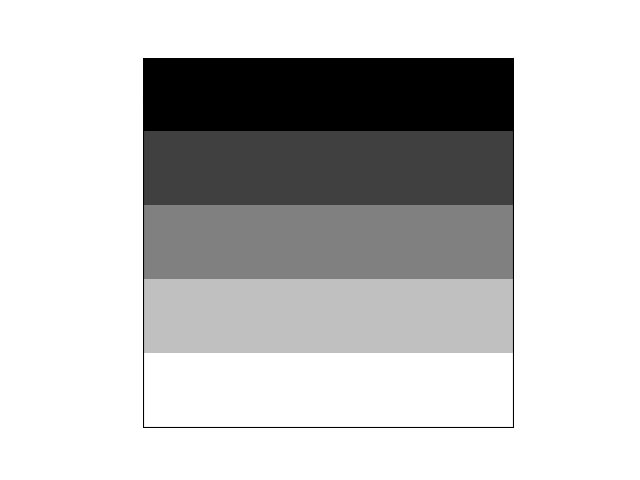
\includegraphics[scale=0.5]{images/arbitrary_tiles.png}
    \fautor
\end{figure*}

The DFT transforms $I$ into a set of Fourier coefficients, as
\[
\hat{I} = 
\begin{bmatrix}
    12.5 + 0i & 0 + 0i & 0 + 0i & 0 + 0i & 0 + 0i
    \\
    -3.125 + 4.30119i & 0 + 0i & 0 + 0i & 0 + 0i & 0 + 0i
    \\
    -3.125 + 1.01537i & 0 + 0i & 0 + 0i & 0 + 0i & 0 + 0i	
    \\
    -3.125 -1.01537i & 0 + 0i & 0 + 0i & 0 + 0i & 0 + 0i
    \\
    -3.125 -4.30119i & 0 + 0i & 0 + 0i & 0 + 0i & 0 + 0i
\end{bmatrix}.
\]

\noindent Applying $\hat{I}$ in $K$, we obtain the magnitude matrix of the Fourier coefficients from $\hat{I}$, denoted as $M$ and given by

\[
M = 
\begin{bmatrix}
    2.60269 & 0 & 0 & 0 & 0
    \\
    1.84318 & 0 & 0 & 0 & 0	
    \\
    1.45531 & 0 & 0 & 0 & 0	
    \\
    1.45531 & 0 & 0 & 0 & 0	
    \\
    1.84318 & 0 & 0 & 0 & 0	
\end{bmatrix}.
\]

\vspace{0.1in}

\noindent From this result, we may compute the sum of the square of absolute values of $M$ in order to show that the result is finite. Indeed,

\[
\sum_{i=1}^{m}\sum_{j=1}^{n}|M|^{2} \approx 18 < \infty,
\]

\noindent what completes the proof.
\end{proof}
\end{theorem}
\end{apendicesenv}

\end{document}